% Options for packages loaded elsewhere
% Options for packages loaded elsewhere
\PassOptionsToPackage{unicode}{hyperref}
\PassOptionsToPackage{hyphens}{url}
\PassOptionsToPackage{dvipsnames,svgnames,x11names}{xcolor}
%
\documentclass[
  letterpaper,
  DIV=11,
  numbers=noendperiod]{scrartcl}
\usepackage{xcolor}
\usepackage[margin=1in]{geometry}
\usepackage{amsmath,amssymb}
\setcounter{secnumdepth}{5}
\usepackage{iftex}
\ifPDFTeX
  \usepackage[T1]{fontenc}
  \usepackage[utf8]{inputenc}
  \usepackage{textcomp} % provide euro and other symbols
\else % if luatex or xetex
  \usepackage{unicode-math} % this also loads fontspec
  \defaultfontfeatures{Scale=MatchLowercase}
  \defaultfontfeatures[\rmfamily]{Ligatures=TeX,Scale=1}
\fi
\usepackage{lmodern}
\ifPDFTeX\else
  % xetex/luatex font selection
\fi
% Use upquote if available, for straight quotes in verbatim environments
\IfFileExists{upquote.sty}{\usepackage{upquote}}{}
\IfFileExists{microtype.sty}{% use microtype if available
  \usepackage[]{microtype}
  \UseMicrotypeSet[protrusion]{basicmath} % disable protrusion for tt fonts
}{}
\makeatletter
\@ifundefined{KOMAClassName}{% if non-KOMA class
  \IfFileExists{parskip.sty}{%
    \usepackage{parskip}
  }{% else
    \setlength{\parindent}{0pt}
    \setlength{\parskip}{6pt plus 2pt minus 1pt}}
}{% if KOMA class
  \KOMAoptions{parskip=half}}
\makeatother
% Make \paragraph and \subparagraph free-standing
\makeatletter
\ifx\paragraph\undefined\else
  \let\oldparagraph\paragraph
  \renewcommand{\paragraph}{
    \@ifstar
      \xxxParagraphStar
      \xxxParagraphNoStar
  }
  \newcommand{\xxxParagraphStar}[1]{\oldparagraph*{#1}\mbox{}}
  \newcommand{\xxxParagraphNoStar}[1]{\oldparagraph{#1}\mbox{}}
\fi
\ifx\subparagraph\undefined\else
  \let\oldsubparagraph\subparagraph
  \renewcommand{\subparagraph}{
    \@ifstar
      \xxxSubParagraphStar
      \xxxSubParagraphNoStar
  }
  \newcommand{\xxxSubParagraphStar}[1]{\oldsubparagraph*{#1}\mbox{}}
  \newcommand{\xxxSubParagraphNoStar}[1]{\oldsubparagraph{#1}\mbox{}}
\fi
\makeatother

\usepackage{color}
\usepackage{fancyvrb}
\newcommand{\VerbBar}{|}
\newcommand{\VERB}{\Verb[commandchars=\\\{\}]}
\DefineVerbatimEnvironment{Highlighting}{Verbatim}{commandchars=\\\{\}}
% Add ',fontsize=\small' for more characters per line
\usepackage{framed}
\definecolor{shadecolor}{RGB}{241,243,245}
\newenvironment{Shaded}{\begin{snugshade}}{\end{snugshade}}
\newcommand{\AlertTok}[1]{\textcolor[rgb]{0.68,0.00,0.00}{#1}}
\newcommand{\AnnotationTok}[1]{\textcolor[rgb]{0.37,0.37,0.37}{#1}}
\newcommand{\AttributeTok}[1]{\textcolor[rgb]{0.40,0.45,0.13}{#1}}
\newcommand{\BaseNTok}[1]{\textcolor[rgb]{0.68,0.00,0.00}{#1}}
\newcommand{\BuiltInTok}[1]{\textcolor[rgb]{0.00,0.23,0.31}{#1}}
\newcommand{\CharTok}[1]{\textcolor[rgb]{0.13,0.47,0.30}{#1}}
\newcommand{\CommentTok}[1]{\textcolor[rgb]{0.37,0.37,0.37}{#1}}
\newcommand{\CommentVarTok}[1]{\textcolor[rgb]{0.37,0.37,0.37}{\textit{#1}}}
\newcommand{\ConstantTok}[1]{\textcolor[rgb]{0.56,0.35,0.01}{#1}}
\newcommand{\ControlFlowTok}[1]{\textcolor[rgb]{0.00,0.23,0.31}{\textbf{#1}}}
\newcommand{\DataTypeTok}[1]{\textcolor[rgb]{0.68,0.00,0.00}{#1}}
\newcommand{\DecValTok}[1]{\textcolor[rgb]{0.68,0.00,0.00}{#1}}
\newcommand{\DocumentationTok}[1]{\textcolor[rgb]{0.37,0.37,0.37}{\textit{#1}}}
\newcommand{\ErrorTok}[1]{\textcolor[rgb]{0.68,0.00,0.00}{#1}}
\newcommand{\ExtensionTok}[1]{\textcolor[rgb]{0.00,0.23,0.31}{#1}}
\newcommand{\FloatTok}[1]{\textcolor[rgb]{0.68,0.00,0.00}{#1}}
\newcommand{\FunctionTok}[1]{\textcolor[rgb]{0.28,0.35,0.67}{#1}}
\newcommand{\ImportTok}[1]{\textcolor[rgb]{0.00,0.46,0.62}{#1}}
\newcommand{\InformationTok}[1]{\textcolor[rgb]{0.37,0.37,0.37}{#1}}
\newcommand{\KeywordTok}[1]{\textcolor[rgb]{0.00,0.23,0.31}{\textbf{#1}}}
\newcommand{\NormalTok}[1]{\textcolor[rgb]{0.00,0.23,0.31}{#1}}
\newcommand{\OperatorTok}[1]{\textcolor[rgb]{0.37,0.37,0.37}{#1}}
\newcommand{\OtherTok}[1]{\textcolor[rgb]{0.00,0.23,0.31}{#1}}
\newcommand{\PreprocessorTok}[1]{\textcolor[rgb]{0.68,0.00,0.00}{#1}}
\newcommand{\RegionMarkerTok}[1]{\textcolor[rgb]{0.00,0.23,0.31}{#1}}
\newcommand{\SpecialCharTok}[1]{\textcolor[rgb]{0.37,0.37,0.37}{#1}}
\newcommand{\SpecialStringTok}[1]{\textcolor[rgb]{0.13,0.47,0.30}{#1}}
\newcommand{\StringTok}[1]{\textcolor[rgb]{0.13,0.47,0.30}{#1}}
\newcommand{\VariableTok}[1]{\textcolor[rgb]{0.07,0.07,0.07}{#1}}
\newcommand{\VerbatimStringTok}[1]{\textcolor[rgb]{0.13,0.47,0.30}{#1}}
\newcommand{\WarningTok}[1]{\textcolor[rgb]{0.37,0.37,0.37}{\textit{#1}}}

\usepackage{longtable,booktabs,array}
\usepackage{calc} % for calculating minipage widths
% Correct order of tables after \paragraph or \subparagraph
\usepackage{etoolbox}
\makeatletter
\patchcmd\longtable{\par}{\if@noskipsec\mbox{}\fi\par}{}{}
\makeatother
% Allow footnotes in longtable head/foot
\IfFileExists{footnotehyper.sty}{\usepackage{footnotehyper}}{\usepackage{footnote}}
\makesavenoteenv{longtable}
\usepackage{graphicx}
\makeatletter
\newsavebox\pandoc@box
\newcommand*\pandocbounded[1]{% scales image to fit in text height/width
  \sbox\pandoc@box{#1}%
  \Gscale@div\@tempa{\textheight}{\dimexpr\ht\pandoc@box+\dp\pandoc@box\relax}%
  \Gscale@div\@tempb{\linewidth}{\wd\pandoc@box}%
  \ifdim\@tempb\p@<\@tempa\p@\let\@tempa\@tempb\fi% select the smaller of both
  \ifdim\@tempa\p@<\p@\scalebox{\@tempa}{\usebox\pandoc@box}%
  \else\usebox{\pandoc@box}%
  \fi%
}
% Set default figure placement to htbp
\def\fps@figure{htbp}
\makeatother





\setlength{\emergencystretch}{3em} % prevent overfull lines

\providecommand{\tightlist}{%
  \setlength{\itemsep}{0pt}\setlength{\parskip}{0pt}}



 


\KOMAoption{captions}{tableheading}
\makeatletter
\@ifpackageloaded{tcolorbox}{}{\usepackage[skins,breakable]{tcolorbox}}
\@ifpackageloaded{fontawesome5}{}{\usepackage{fontawesome5}}
\definecolor{quarto-callout-color}{HTML}{909090}
\definecolor{quarto-callout-note-color}{HTML}{0758E5}
\definecolor{quarto-callout-important-color}{HTML}{CC1914}
\definecolor{quarto-callout-warning-color}{HTML}{EB9113}
\definecolor{quarto-callout-tip-color}{HTML}{00A047}
\definecolor{quarto-callout-caution-color}{HTML}{FC5300}
\definecolor{quarto-callout-color-frame}{HTML}{acacac}
\definecolor{quarto-callout-note-color-frame}{HTML}{4582ec}
\definecolor{quarto-callout-important-color-frame}{HTML}{d9534f}
\definecolor{quarto-callout-warning-color-frame}{HTML}{f0ad4e}
\definecolor{quarto-callout-tip-color-frame}{HTML}{02b875}
\definecolor{quarto-callout-caution-color-frame}{HTML}{fd7e14}
\makeatother
\makeatletter
\@ifpackageloaded{caption}{}{\usepackage{caption}}
\AtBeginDocument{%
\ifdefined\contentsname
  \renewcommand*\contentsname{Table of contents}
\else
  \newcommand\contentsname{Table of contents}
\fi
\ifdefined\listfigurename
  \renewcommand*\listfigurename{List of Figures}
\else
  \newcommand\listfigurename{List of Figures}
\fi
\ifdefined\listtablename
  \renewcommand*\listtablename{List of Tables}
\else
  \newcommand\listtablename{List of Tables}
\fi
\ifdefined\figurename
  \renewcommand*\figurename{Figure}
\else
  \newcommand\figurename{Figure}
\fi
\ifdefined\tablename
  \renewcommand*\tablename{Table}
\else
  \newcommand\tablename{Table}
\fi
}
\@ifpackageloaded{float}{}{\usepackage{float}}
\floatstyle{ruled}
\@ifundefined{c@chapter}{\newfloat{codelisting}{h}{lop}}{\newfloat{codelisting}{h}{lop}[chapter]}
\floatname{codelisting}{Listing}
\newcommand*\listoflistings{\listof{codelisting}{List of Listings}}
\makeatother
\makeatletter
\makeatother
\makeatletter
\@ifpackageloaded{caption}{}{\usepackage{caption}}
\@ifpackageloaded{subcaption}{}{\usepackage{subcaption}}
\makeatother
\usepackage{bookmark}
\IfFileExists{xurl.sty}{\usepackage{xurl}}{} % add URL line breaks if available
\urlstyle{same}
\hypersetup{
  pdftitle={Ecosystem Service Change \& Hotspot Extraction},
  pdfauthor={Jerónimo Rodríguez Escobar},
  colorlinks=true,
  linkcolor={blue},
  filecolor={Maroon},
  citecolor={Blue},
  urlcolor={Blue},
  pdfcreator={LaTeX via pandoc}}


\title{Ecosystem Service Change \& Hotspot Extraction}
\usepackage{etoolbox}
\makeatletter
\providecommand{\subtitle}[1]{% add subtitle to \maketitle
  \apptocmd{\@title}{\par {\large #1 \par}}{}{}
}
\makeatother
\subtitle{vv1.3.1}
\author{Jerónimo Rodríguez Escobar}
\date{2026-04-30 06:41 Pacific Daylight Time}
\begin{document}
\maketitle

\renewcommand*\contentsname{Table of contents}
{
\hypersetup{linkcolor=}
\setcounter{tocdepth}{3}
\tableofcontents
}

\section{Overview}\label{overview}

Derives hotspot flags and produces bar/violin plots summarizing change
by subregion. Assumes process\_data.qmd has been run first to produce
the canonical grid + change dataset (10k\_change\_calc.gpkg). Key steps:
load the canonical grid, pivot change fields to long form, define
hotspots using the configured thresholds, export hotspot layers, and
save plots to outputs/plots/.

\begin{tcolorbox}[enhanced jigsaw, colframe=quarto-callout-tip-color-frame, colback=white, leftrule=.75mm, left=2mm, bottomrule=.15mm, arc=.35mm, toprule=.15mm, coltitle=black, rightrule=.15mm, opacityback=0, breakable, toptitle=1mm, opacitybacktitle=0.6, bottomtitle=1mm, colbacktitle=quarto-callout-tip-color!10!white, title=\textcolor{quarto-callout-tip-color}{\faLightbulb}\hspace{0.5em}{Future Tasks \& Ideas}, titlerule=0mm]

Here are some ideas and future tasks for this analysis:

\begin{enumerate}
\def\labelenumi{\arabic{enumi}.}
\tightlist
\item
  \textbf{Adapt analysis for multi-temporal data:} Adapt analysis to
  handle updated modeled ES layers and multiple points in time (beyond
  bi-temporal T0, T1). Strategize for incorporating multi-temporal data.
\item
  \textbf{Quantify hotspot vs.~non-hotspot change:} Develop a method to
  quantify and visualize the share of total change (from bar plots) that
  occurs within hotspots versus outside of them, possibly using stacked
  bar plots.
\item
  \textbf{Simplify Spatial Joins (V2 Technical Debt):} Remove the
  on-the-fly spatial coordinate joins (X/Y) used to bypass upstream
  row-shifting. Once \texttt{summary\_pipeline\_landgrid.py} is updated
  to preserve true FIDs, revert to standard tabular
  \texttt{left\_join(by\ =\ "fid")}.
\end{enumerate}

\end{tcolorbox}

\section{Setup and Libraries}\label{setup-and-libraries}

Load all core packages (tidyverse, spatial, plotting helpers) and
initialize reproducibility settings. This chunk also sources
\texttt{R/paths.R} and runs \texttt{devtools::load\_all()} so downstream
chunks can reuse helper functions.

\section{Metadata Banner}\label{metadata-banner}

Published: 2026-04-30 06:42 PDT

\begin{tcolorbox}[enhanced jigsaw, colframe=quarto-callout-note-color-frame, colback=white, leftrule=.75mm, left=2mm, bottomrule=.15mm, arc=.35mm, toprule=.15mm, coltitle=black, rightrule=.15mm, opacityback=0, breakable, toptitle=1mm, opacitybacktitle=0.6, bottomtitle=1mm, colbacktitle=quarto-callout-note-color!10!white, title=\textcolor{quarto-callout-note-color}{\faInfo}\hspace{0.5em}{Note}, titlerule=0mm]

\textbf{Run metadata}

\begin{itemize}
\tightlist
\item
  Analysis version: v1.3.1
\item
  Rendered: 2026-04-30 06:42 PDT
\item
  Git: feature/equity-and-drivers @ 1a40bcc
\item
  Data root: /home/jeronimo/data/global\_ncp
\end{itemize}

\end{tcolorbox}

\section{Produce signed change bars}\label{produce-signed-change-bars}

Bars are computed directly from
\texttt{processed/10k\_change\_calc.gpkg}. We focus specifically on
``active areas'' by dropping true zeros, ensuring that our regional
summaries reflect areas where the ecosystem service is actually provided
or changing. Both absolute and relative changes are plotted with trimmed
tails and a dashed global mean. We no longer compute ``zeros kept''
variants, as discrepancies in sign direction (MAUP/Simpson's Paradox)
are a known property of spatial aggregation rather than an artifact of
zero-handling.

What this chunk does: - Read the processed GPKG and normalize IDs
(\texttt{fid}, \texttt{c\_fid}), dropping any \texttt{c\_fid.x/y}
artifacts. - Build a service mapping (\texttt{svc\_map}) so raw column
bases (with/without \texttt{\_mean}) map to the canonical services;
construct \texttt{col\_pct}/\texttt{col\_abs} names. -
\texttt{agg\_by\_group()}: intersect requested \texttt{groupings} with
available columns; for each grouping × service, pick the pct/abs change
column, drop zeros (\texttt{drop\_zero\ =\ TRUE}), trim extremes at
\texttt{cut\_q}, then compute mean change by group. Returns tidy rows. -
Run \texttt{agg\_by\_group()} to produce \texttt{signed\_summary} and a
later chunk computes global references \texttt{glob\_refs}.

\begin{verbatim}
Grouping 'income_grp': 0 NAs out of 1691786 rows (0%)
  Sample values:  5. Low income, 2. High income: nonOECD, 3. Upper middle income, 4. Lower middle income, 1. High income: OECD 
Grouping 'region_wb': 0 NAs out of 1691786 rows (0%)
  Sample values:  South Asia, Middle East & North Africa, Latin America & Caribbean, Europe & Central Asia, Sub-Saharan Africa 
Grouping 'WWF_biome': 11960 NAs out of 1691786 rows (0.7%)
  Sample values:  Temperate Grasslands, Savannas & Shrublands, Tropical & Subtropical Moist Broadleaf Forests, Temperate Conifer Forests, Tropical & Subtropical Coniferous Forests, Rock & Ice 
\end{verbatim}

\begin{verbatim}
Dimensions of sf_f before filtering:  1691786 x 32 
\end{verbatim}

\begin{verbatim}
Dimensions of sf_subset after filtering:  1526171 x 32 
\end{verbatim}

\begin{verbatim}
Filtered out  165615  rows.
\end{verbatim}

\begin{verbatim}
# A tibble: 48 x 4
   grouping  metric service              n
   <chr>     <chr>  <chr>            <int>
 1 WWF_biome abs    C_Risk              14
 2 WWF_biome abs    C_Risk_Red_Ratio    14
 3 WWF_biome abs    N_Ret_Ratio         14
 4 WWF_biome abs    N_export            14
 5 WWF_biome abs    Nature_Access       14
 6 WWF_biome abs    Pollination         14
 7 WWF_biome abs    Sed_Ret_Ratio       14
 8 WWF_biome abs    Sed_export          14
 9 WWF_biome pct    C_Risk              14
10 WWF_biome pct    C_Risk_Red_Ratio    14
# i 38 more rows
\end{verbatim}

\section{Load cached long table (plt\_long) for
hotspots/KS}\label{load-cached-long-table-plt_long-for-hotspotsks}

\begin{tcolorbox}[enhanced jigsaw, colframe=quarto-callout-note-color-frame, colback=white, leftrule=.75mm, left=2mm, bottomrule=.15mm, arc=.35mm, toprule=.15mm, coltitle=black, rightrule=.15mm, opacityback=0, breakable, toptitle=1mm, opacitybacktitle=0.6, bottomtitle=1mm, colbacktitle=quarto-callout-note-color!10!white, title=\textcolor{quarto-callout-note-color}{\faInfo}\hspace{0.5em}{Note}, titlerule=0mm]

\textbf{Data sharing and external validation}

The pivoted long table (\texttt{plt\_long}) is exported as an RDS file
to the processed data directory (e.g.,
\texttt{/home/jeronimo/data/global\_ncp/processed/plt\_long.rds}). This
file contains all per-cell, per-service change metrics and is the
canonical input for hotspot and KS analyses.

\begin{itemize}
\item
  \textbf{For R users:} Load with:

\begin{Shaded}
\begin{Highlighting}[]
\FunctionTok{source}\NormalTok{(}\StringTok{"R/config.R"}\NormalTok{) }\CommentTok{\# to load cfg object}
\NormalTok{plt\_long }\OtherTok{\textless{}{-}} \FunctionTok{readRDS}\NormalTok{(}\FunctionTok{file.path}\NormalTok{(cfg}\SpecialCharTok{$}\NormalTok{paths}\SpecialCharTok{$}\NormalTok{processed\_data\_dir, }\StringTok{"plt\_long.rds"}\NormalTok{))}
\end{Highlighting}
\end{Shaded}
\item
  \textbf{For Python users:} Use \texttt{pyreadr}
  (\texttt{pip\ install\ pyreadr}), e.g.:

\begin{Shaded}
\begin{Highlighting}[]
\ImportTok{import}\NormalTok{ pyreadr}
\CommentTok{\# Note: You may need to define the path manually if not running in an R{-}integrated environment}
\NormalTok{processed\_data\_dir }\OperatorTok{=} \StringTok{"/home/jeronimo/data/global\_ncp/processed"}
\NormalTok{result }\OperatorTok{=}\NormalTok{ pyreadr.read\_r(}\SpecialStringTok{f\textquotesingle{}}\SpecialCharTok{\{}\NormalTok{processed\_data\_dir}\SpecialCharTok{\}}\SpecialStringTok{/plt\_long.rds\textquotesingle{}}\NormalTok{)}
\NormalTok{df }\OperatorTok{=}\NormalTok{ result[}\VariableTok{None}\NormalTok{]}
\end{Highlighting}
\end{Shaded}
\item
  \textbf{For other tools:} RDS is a binary format; consider converting
  to CSV or Feather for broader compatibility if needed.
\end{itemize}

This object is suitable for external review, reproducibility checks, and
further interpretation in any suitable software.

\end{tcolorbox}

Hotspot export and KS still expect \texttt{plt\_long}. To avoid the
heavy pivot here, we load the cached table from the processed data
directory. If it's missing, this script can regenerate it.

\section{Hotspot extraction workflow (global +
subregional)}\label{hotspot-extraction-workflow-global-subregional}

We identify per-service hotspots using a 5\% percentile rule and
\textbf{direction vectors}: - \texttt{loss\_services} (e.g.,
Nature\_Access, Pollination, N/Sed\_Ret\_Ratio, C\_Risk\_Red\_Ratio) →
we flag the \textbf{lowest} values; - \texttt{gain\_services}
(Sed\_export, N\_export, C\_Risk) → we flag the \textbf{highest} values.
\textbf{Definition of a Hotspot:} A hotspot is defined as a grid cell
representing the \textbf{most detrimental 5\% of change} globally for a
given service.

\begin{itemize}
\tightlist
\item
  \textbf{For Beneficial Services} (e.g., Nature Access, Pollination,
  Retention Ratios): Hotspots are cells with the \textbf{steepest
  declines} (bottom 5\% of the distribution).
\item
  \textbf{For Detrimental Flows/Risks} (e.g., N/Sed Export, Coastal
  Risk): Hotspots are cells with the \textbf{steepest increases} (top
  5\% of the distribution).
\end{itemize}

We run this \textbf{once globally} and then \textbf{once per subregion}
(World Bank region, income group, WWF biome). For each run and for each
metric (absolute and percent change) we write a compact \textbf{GPKG}
containing only the hotspot cells, plus a CSV index:

\begin{itemize}
\tightlist
\item
  Output root: \texttt{processed/hotspots/}

  \begin{itemize}
  \tightlist
  \item
    \texttt{abs/global/hotspots\_global\_abs.gpkg}
  \item
    \texttt{pct/global/hotspots\_global\_pct.gpkg}
  \item
    \texttt{abs/\textless{}group\_col\textgreater{}/hotspots\_\textless{}group\_col\textgreater{}\_\textless{}group\_val\textgreater{}\_abs.gpkg}
  \item
    \texttt{pct/\textless{}group\_col\textgreater{}/hotspots\_\textless{}group\_col\textgreater{}\_\textless{}group\_val\textgreater{}\_pct.gpkg}
  \end{itemize}
\item
  Index: \texttt{processed/hotspots/\_hotspots\_index.csv} (columns:
  scope, group\_col, group\_val, metric, n\_hot, gpkg).
\end{itemize}

These files are meant for QGIS/QA and downstream stats (e.g., KS)
without recomputing hotspots.

\subsection{Hotspot rules \& export
configuration}\label{hotspot-rules-export-configuration}

The analysis uses a single, central configuration so the hotspot rules
are consistent everywhere:

Thresholding: we flag hotspots using the top/bottom tails of the
distribution per service. Here we use a percentile cutoff (e.g., 5\%)
rather than a fixed count.

Direction of concern: services in loss are ``worse when they go down''
(we keep the lowest tail); services in gain are ``worse when they go
up'' (we keep the highest tail).

Combos (optional): grouped service sets that we count per cell for quick
composite summaries.

Export switches: choose whether to write GPKGs and/or the CSV index.

\begin{verbatim}
::: callout-note
**Hotspot configuration**

- Cutoff: 5% (percent)
- Rule mode: vectors
- Loss services: Nature_Access, Pollination, N_Ret_Ratio, Sed_Ret_Ratio, C_Risk_Red_Ratio
- Gain services: Sed_export, N_export, C_Risk
- Combos: **deg_combo**: Nature_Access, Pollination, N_export, Sed_export, C_Risk<br>**rec_combo**: Nature_Access, Pollination, N_Ret_Ratio, Sed_Ret_Ratio, C_Risk_Red_Ratio
…
- Groupings: income_grp, region_wb, WWF_biome, nev_name
…- Write layers: TRUE | Write index: TRUE
- Output dir: `/home/jeronimo/data/global_ncp/processed/hotspots`
:::
\end{verbatim}

\subsection{Validate hotspot
configuration}\label{validate-hotspot-configuration}

\subsection{Export hotspot layers}\label{export-hotspot-layers}

\begin{tcolorbox}[enhanced jigsaw, colframe=quarto-callout-note-color-frame, colback=white, leftrule=.75mm, left=2mm, bottomrule=.15mm, arc=.35mm, toprule=.15mm, coltitle=black, rightrule=.15mm, opacityback=0, breakable, toptitle=1mm, opacitybacktitle=0.6, bottomtitle=1mm, colbacktitle=quarto-callout-note-color!10!white, title=\textcolor{quarto-callout-note-color}{\faInfo}\hspace{0.5em}{Note}, titlerule=0mm]

\textbf{Hotspot export module}\\
- Computes hotspot cells once (global + by subregion) for ABS and PCT
change.\\
- Writes compact GPKGs for mapping/QA and maintains
\texttt{\_hotspots\_index.csv}.\\
- Prereqs: \texttt{plt\_long} in memory, \texttt{HOTS\_CFG} defined
(loss/gain/combos/etc.).

\end{tcolorbox}

\subsection{Regional Mean Change (dashed = global
mean)}\label{regional-mean-change-dashed-global-mean}

\pandocbounded{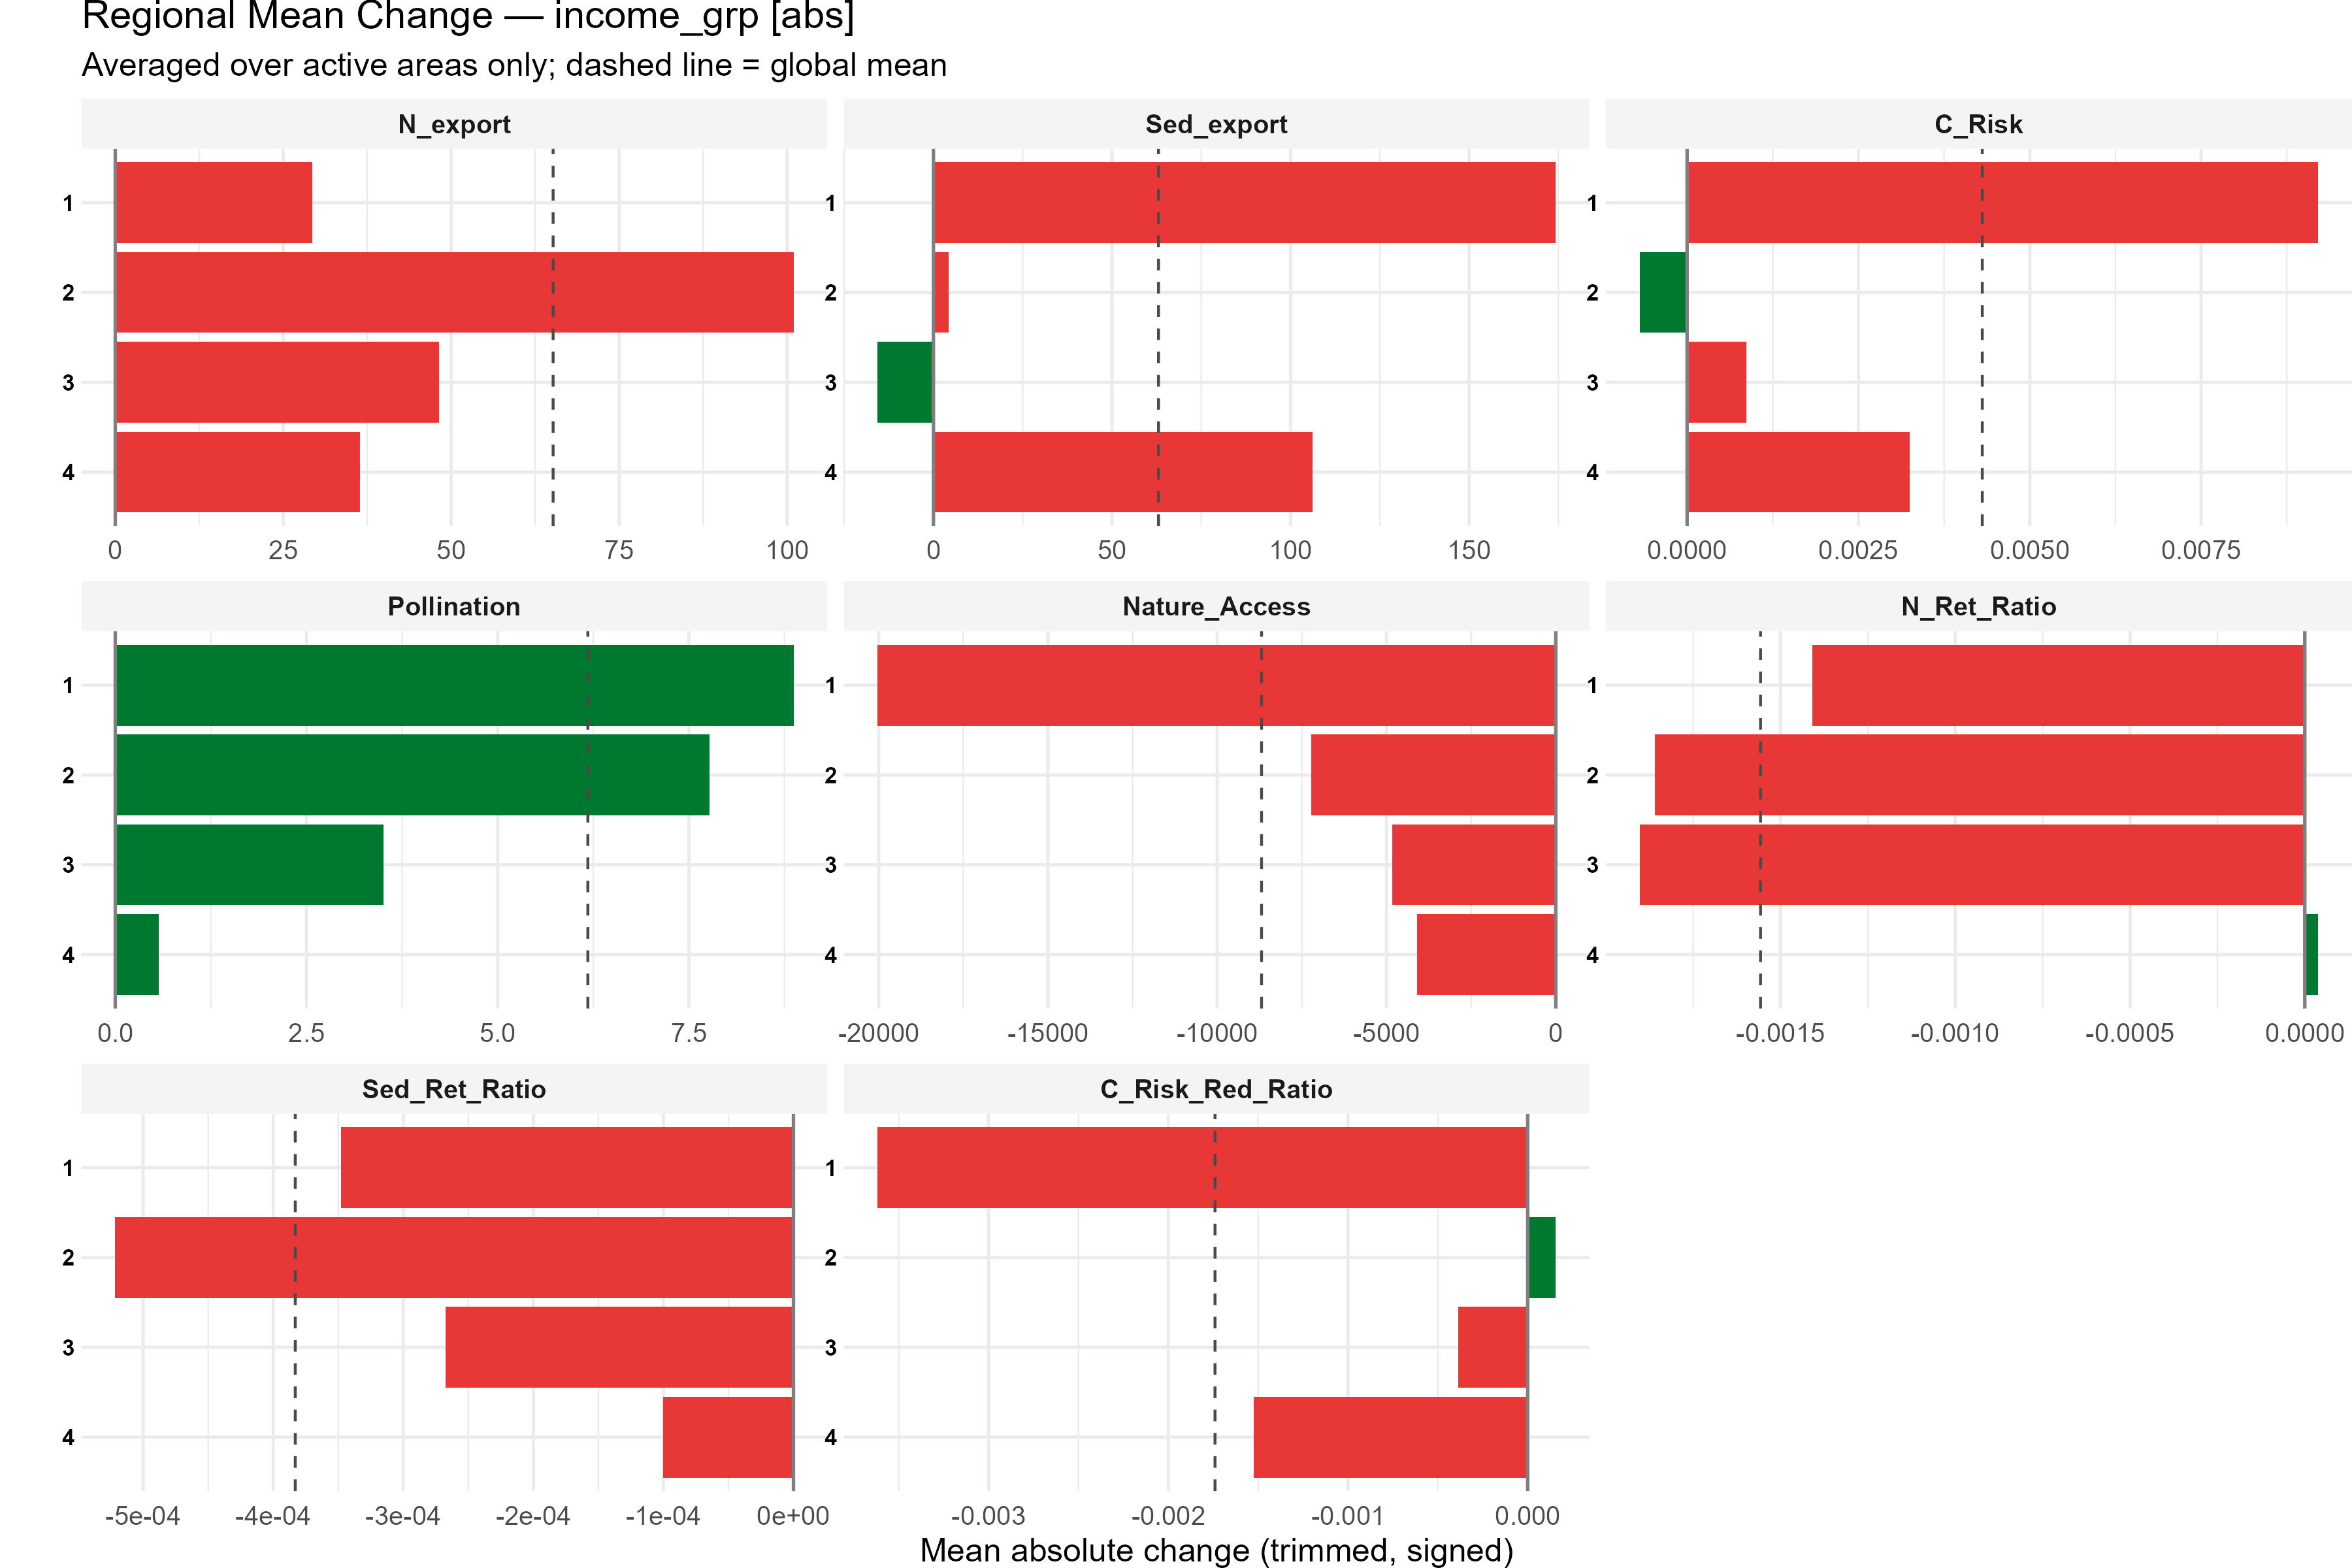
\includegraphics[keepaspectratio]{../outputs/plots/signed_bars/bars_signed_income_grp_abs.png}}

\pandocbounded{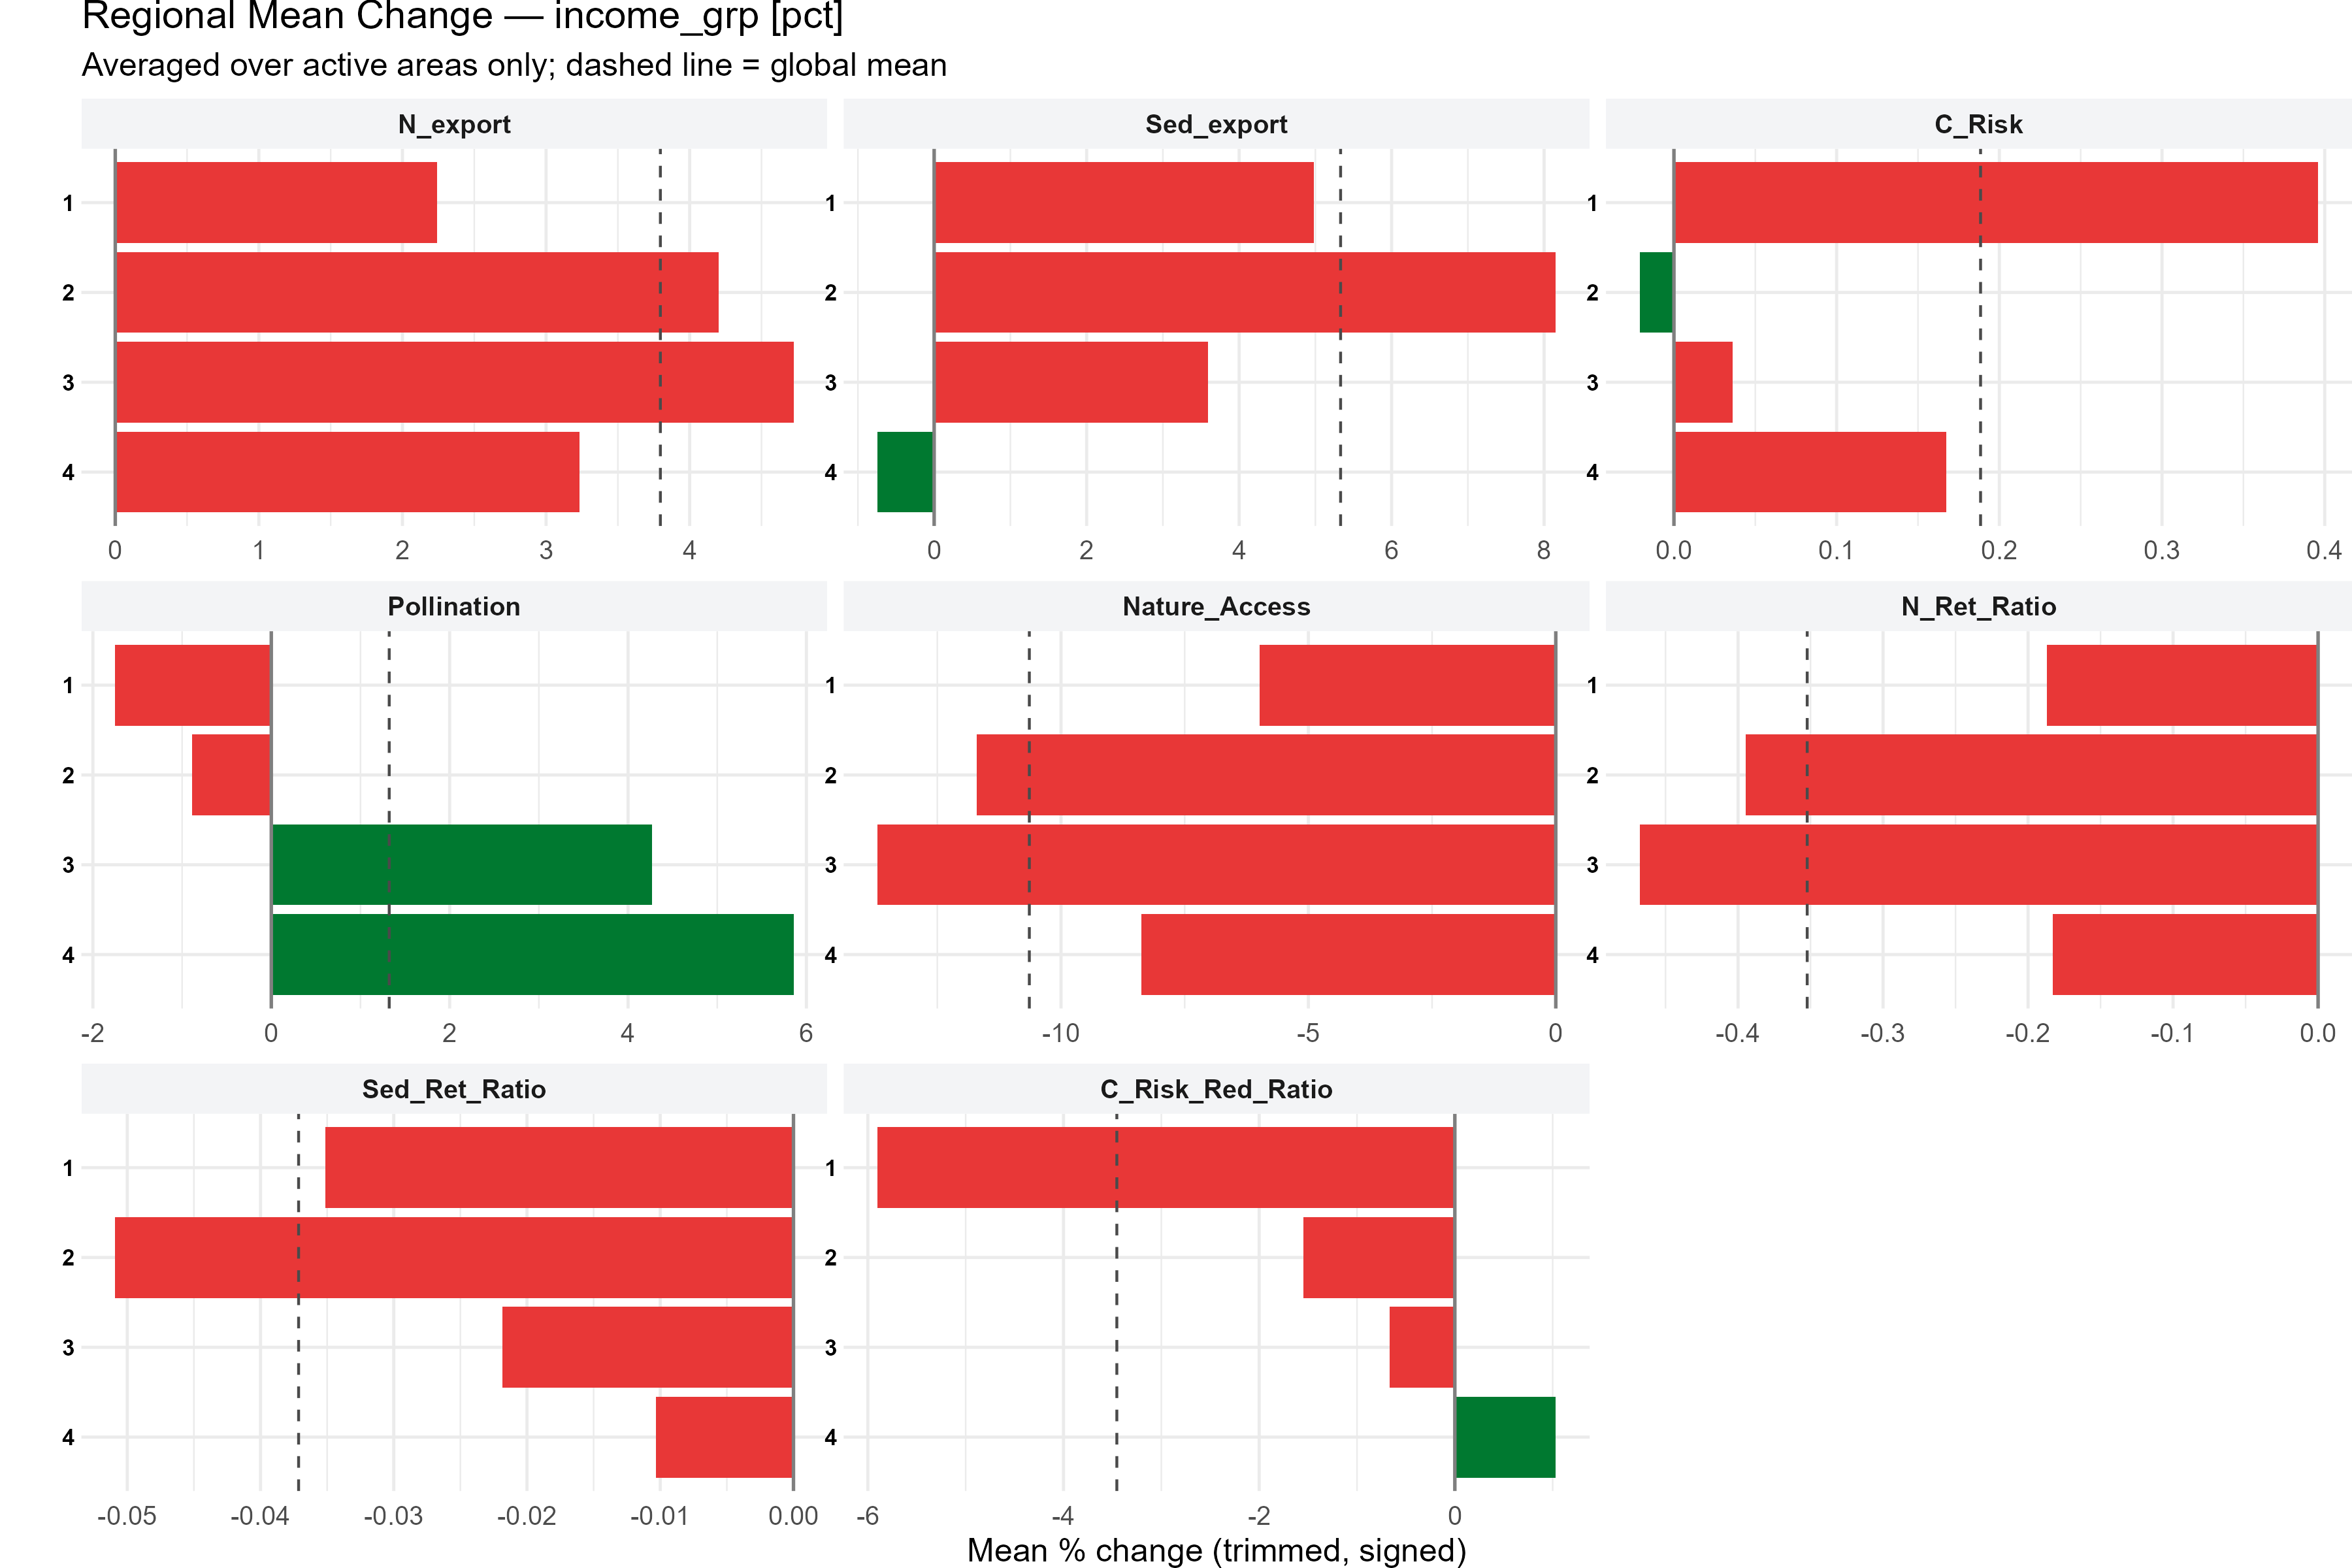
\includegraphics[keepaspectratio]{../outputs/plots/signed_bars/bars_signed_income_grp_pct.png}}

\pandocbounded{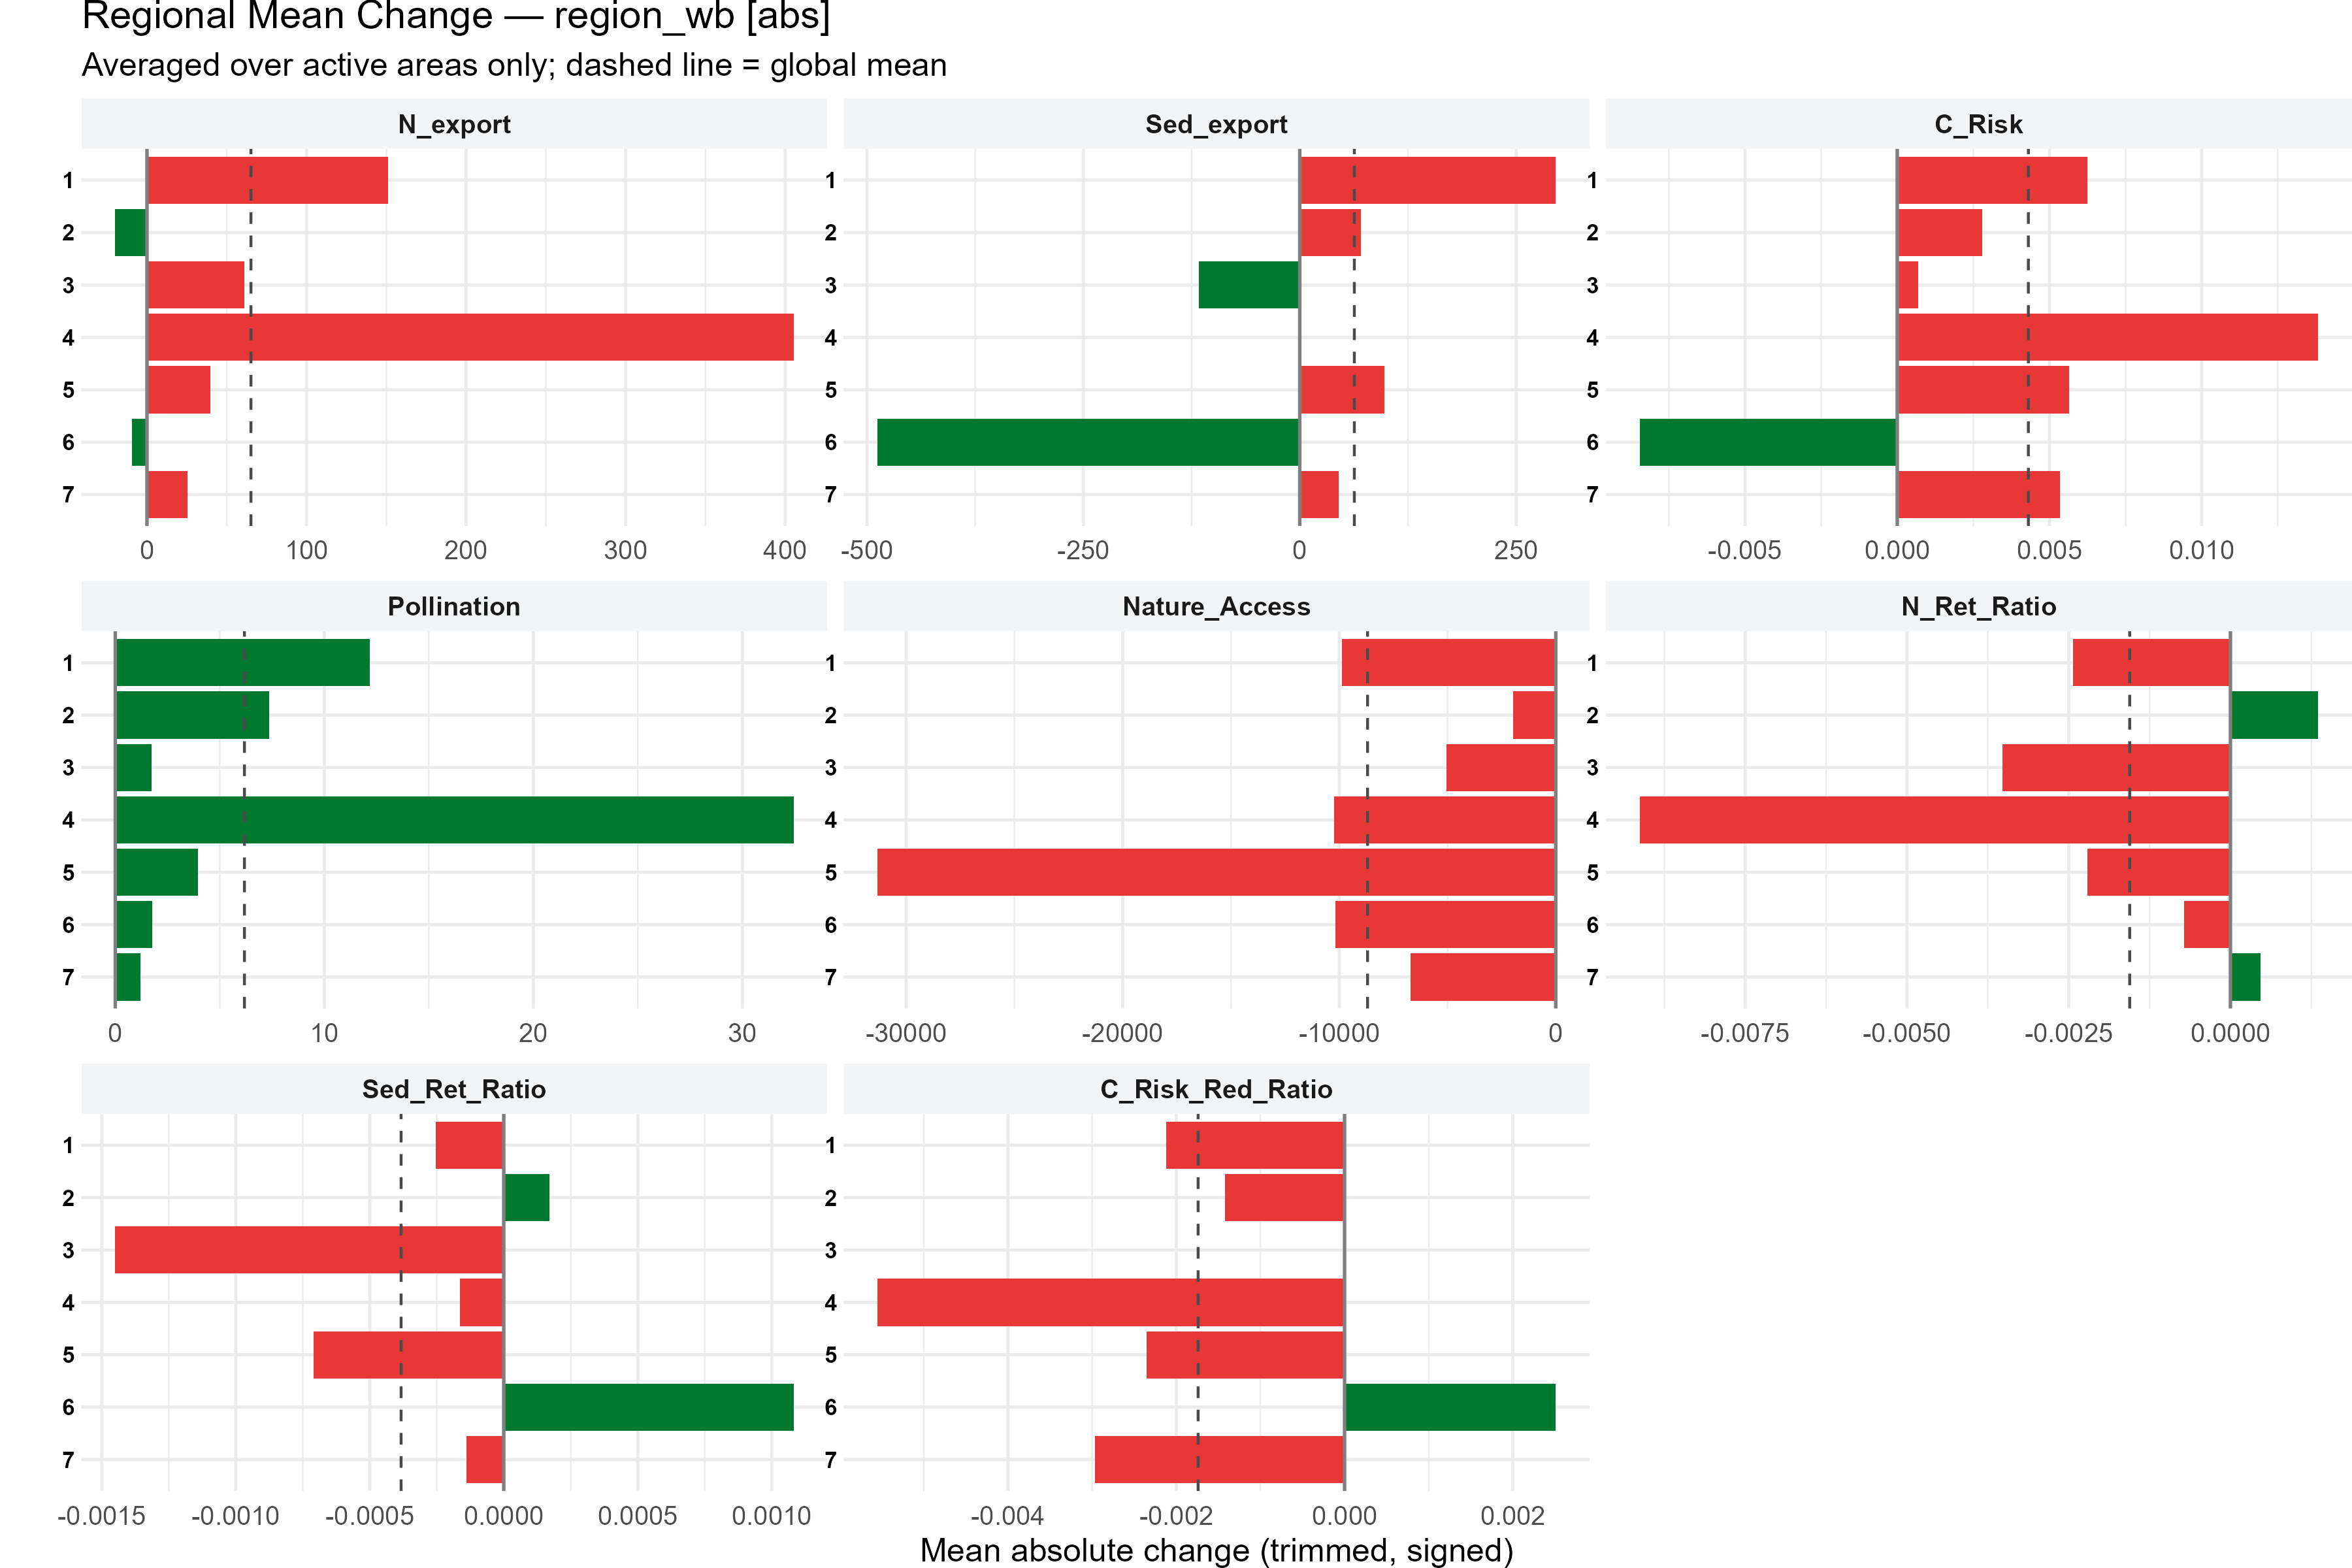
\includegraphics[keepaspectratio]{../outputs/plots/signed_bars/bars_signed_region_wb_abs.png}}

\pandocbounded{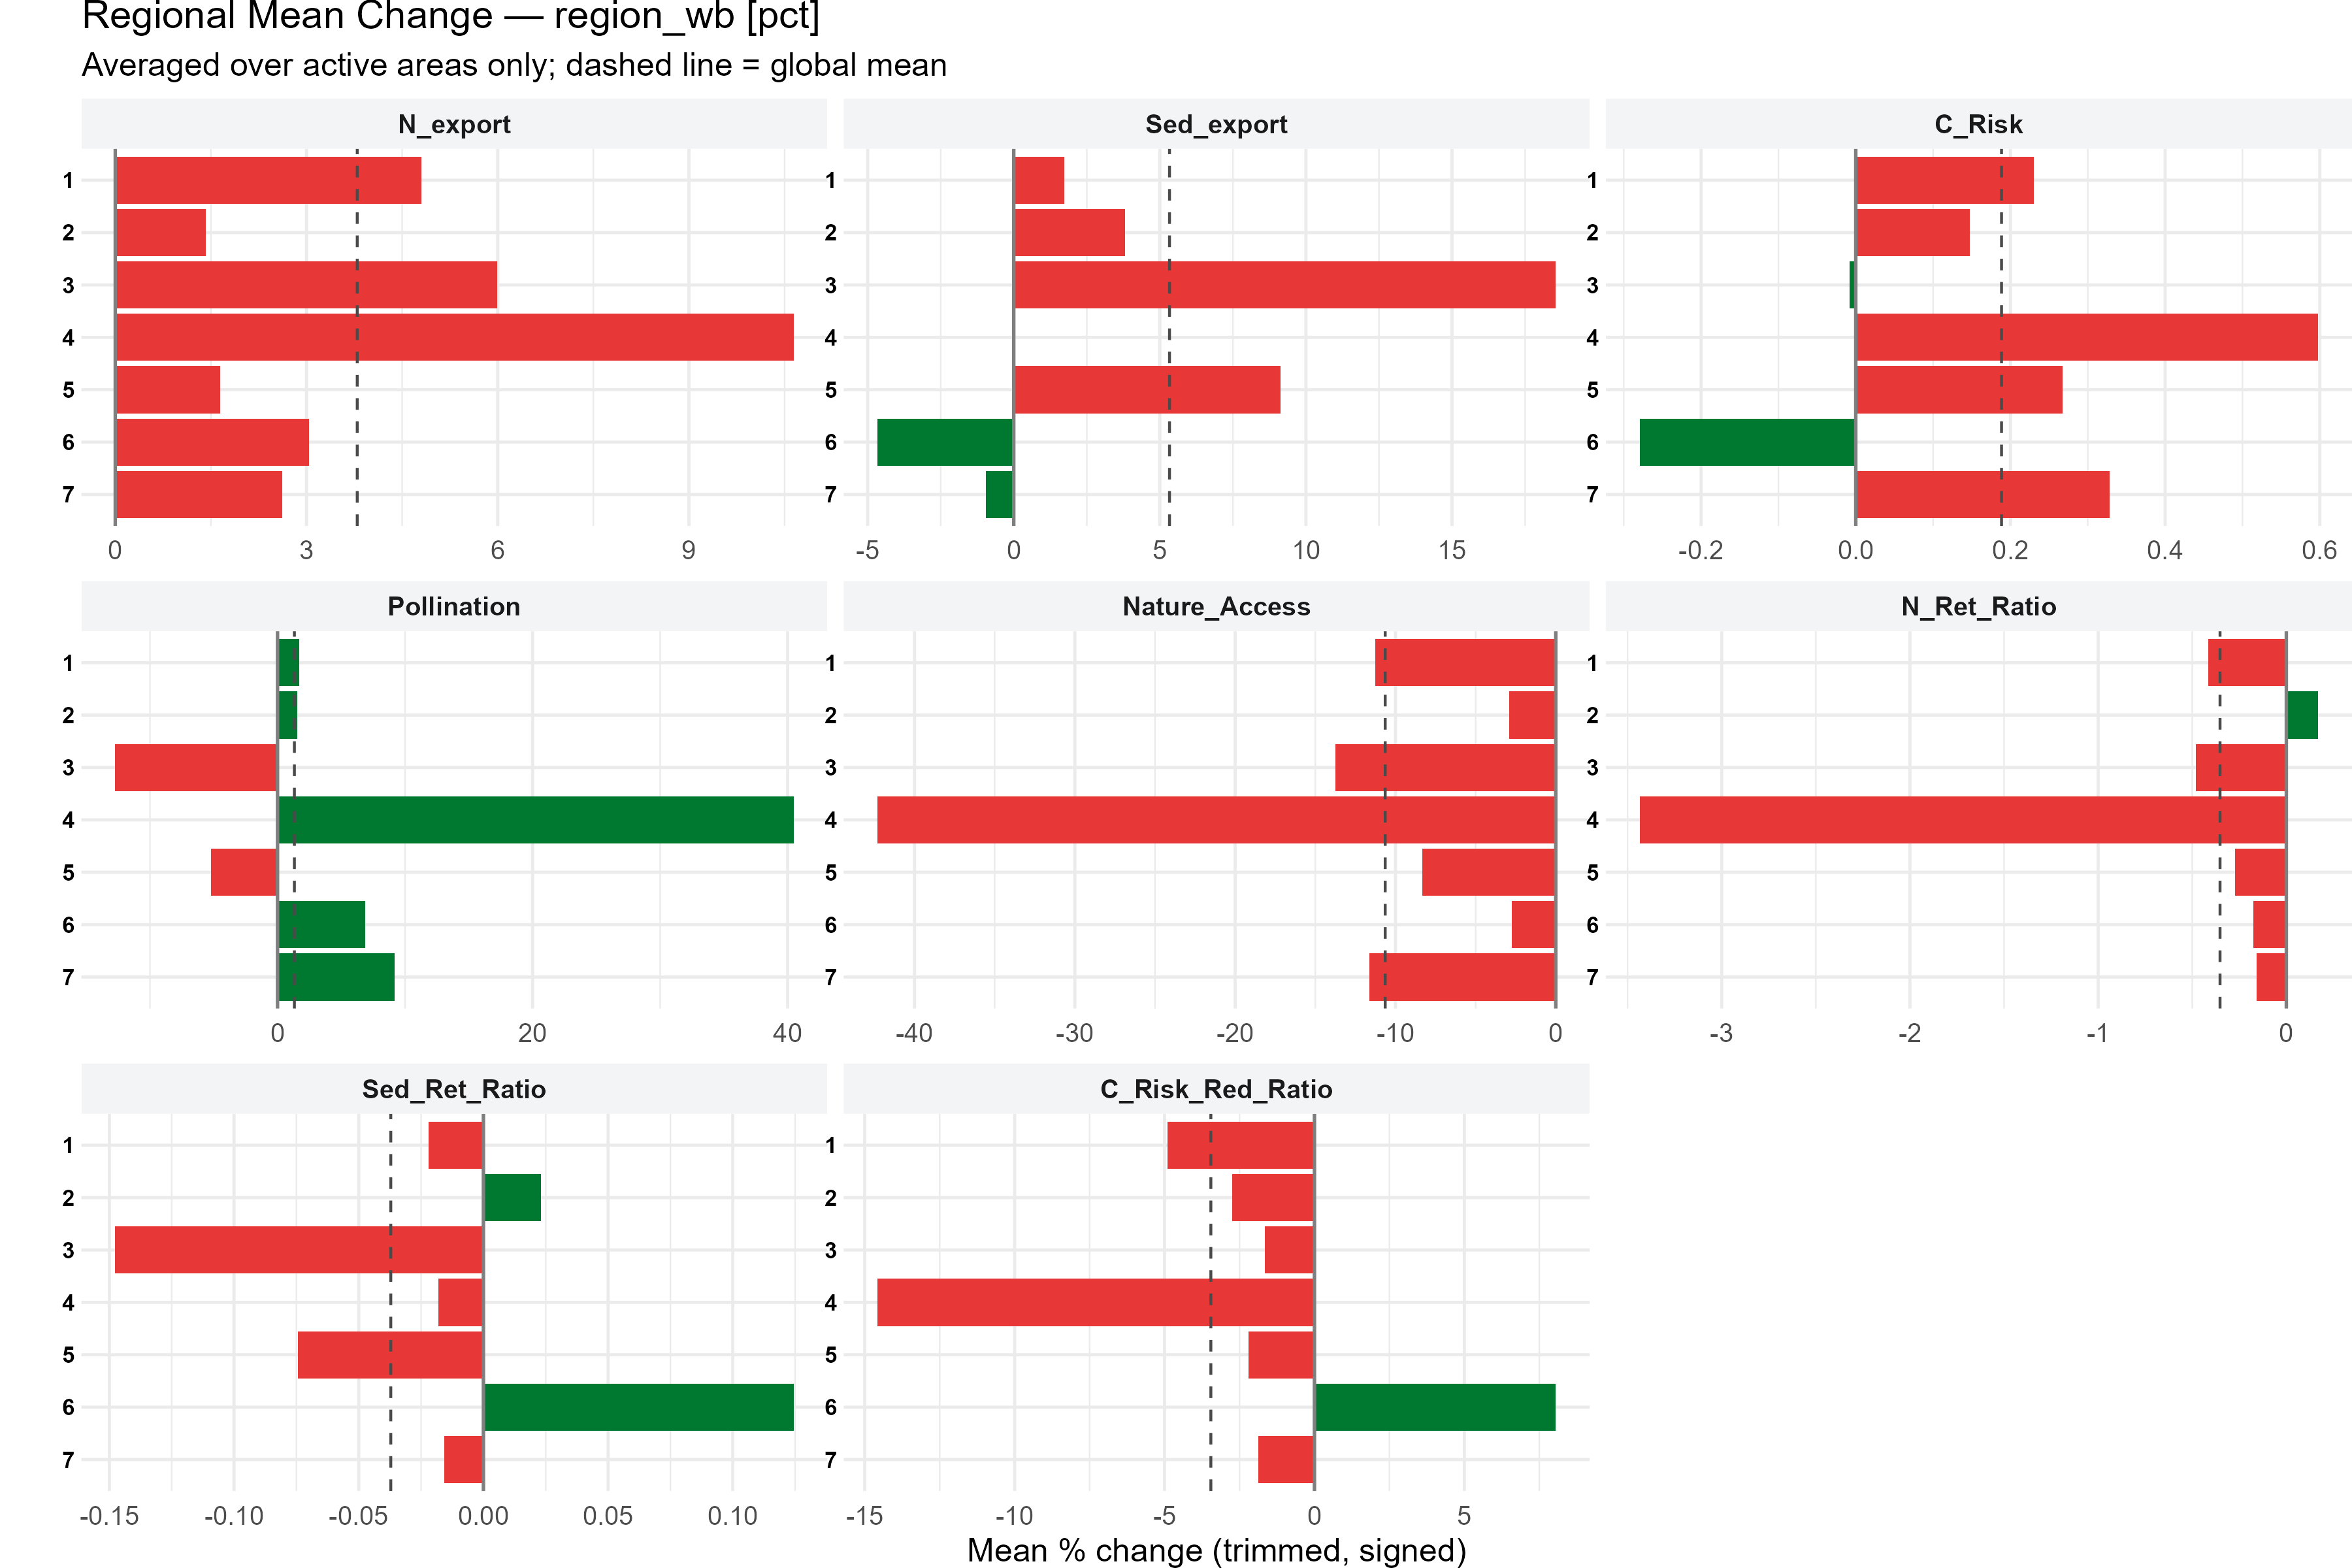
\includegraphics[keepaspectratio]{../outputs/plots/signed_bars/bars_signed_region_wb_pct.png}}

\pandocbounded{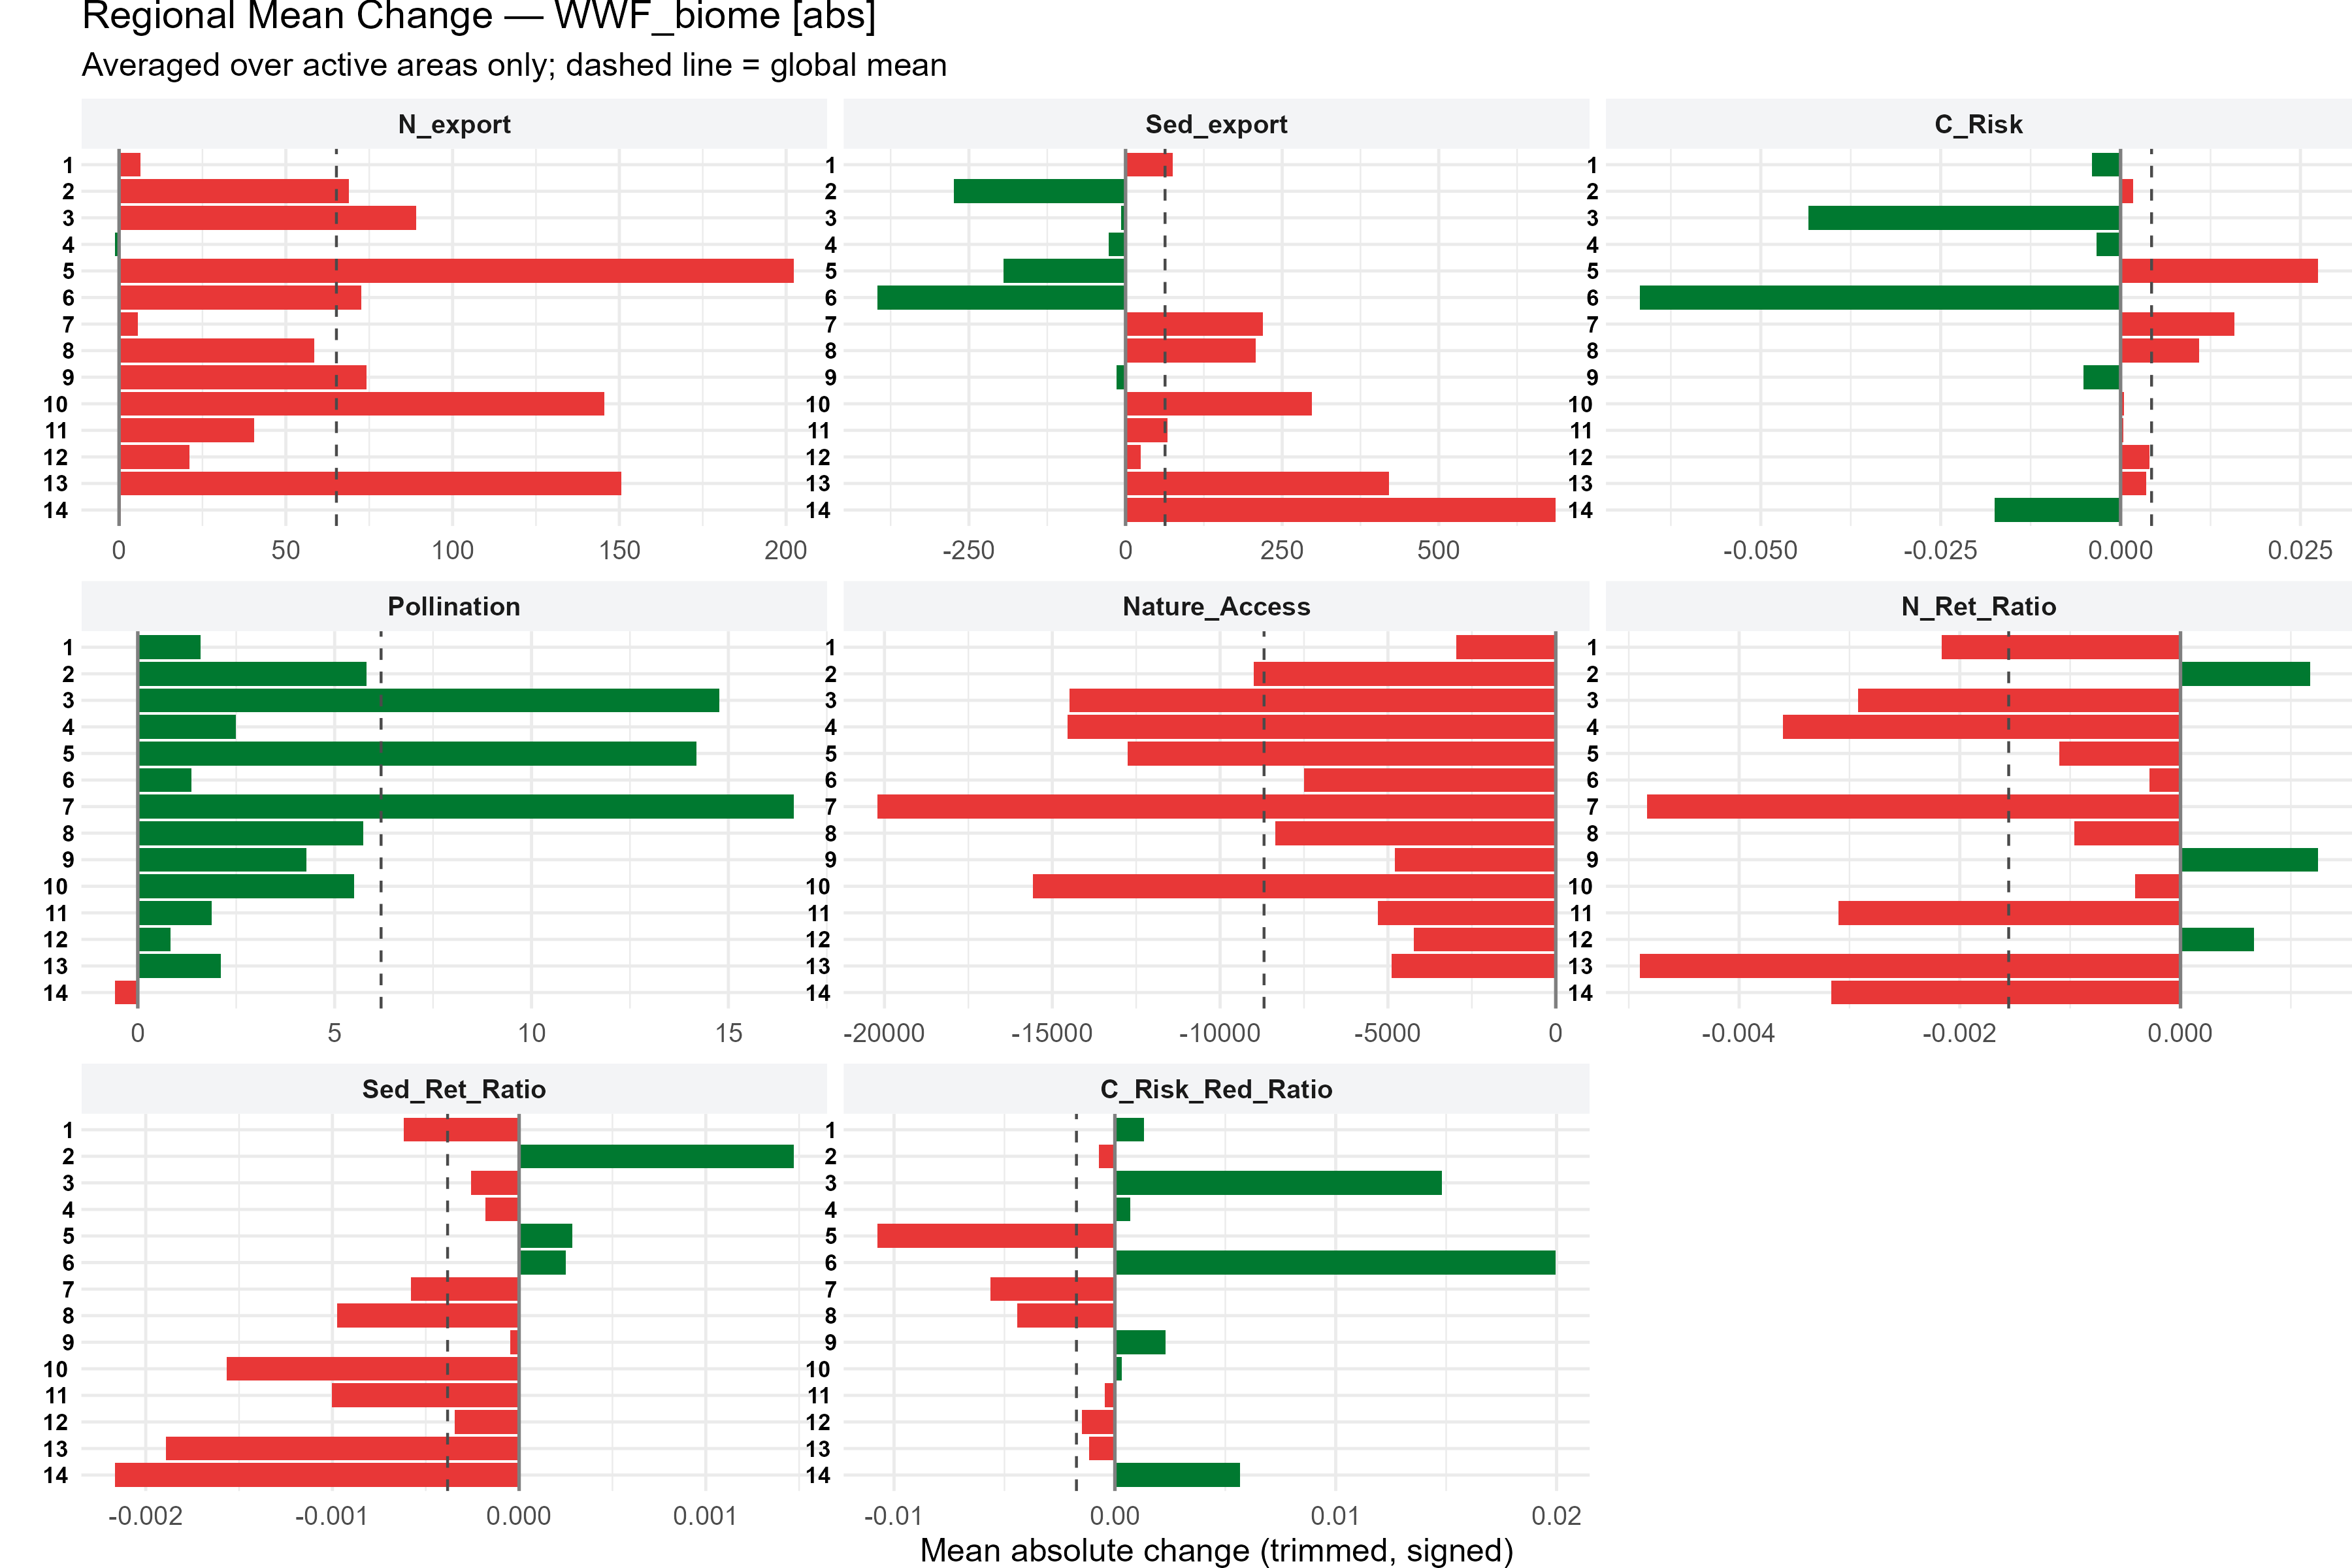
\includegraphics[keepaspectratio]{../outputs/plots/signed_bars/bars_signed_wwf_biome_abs.png}}

\pandocbounded{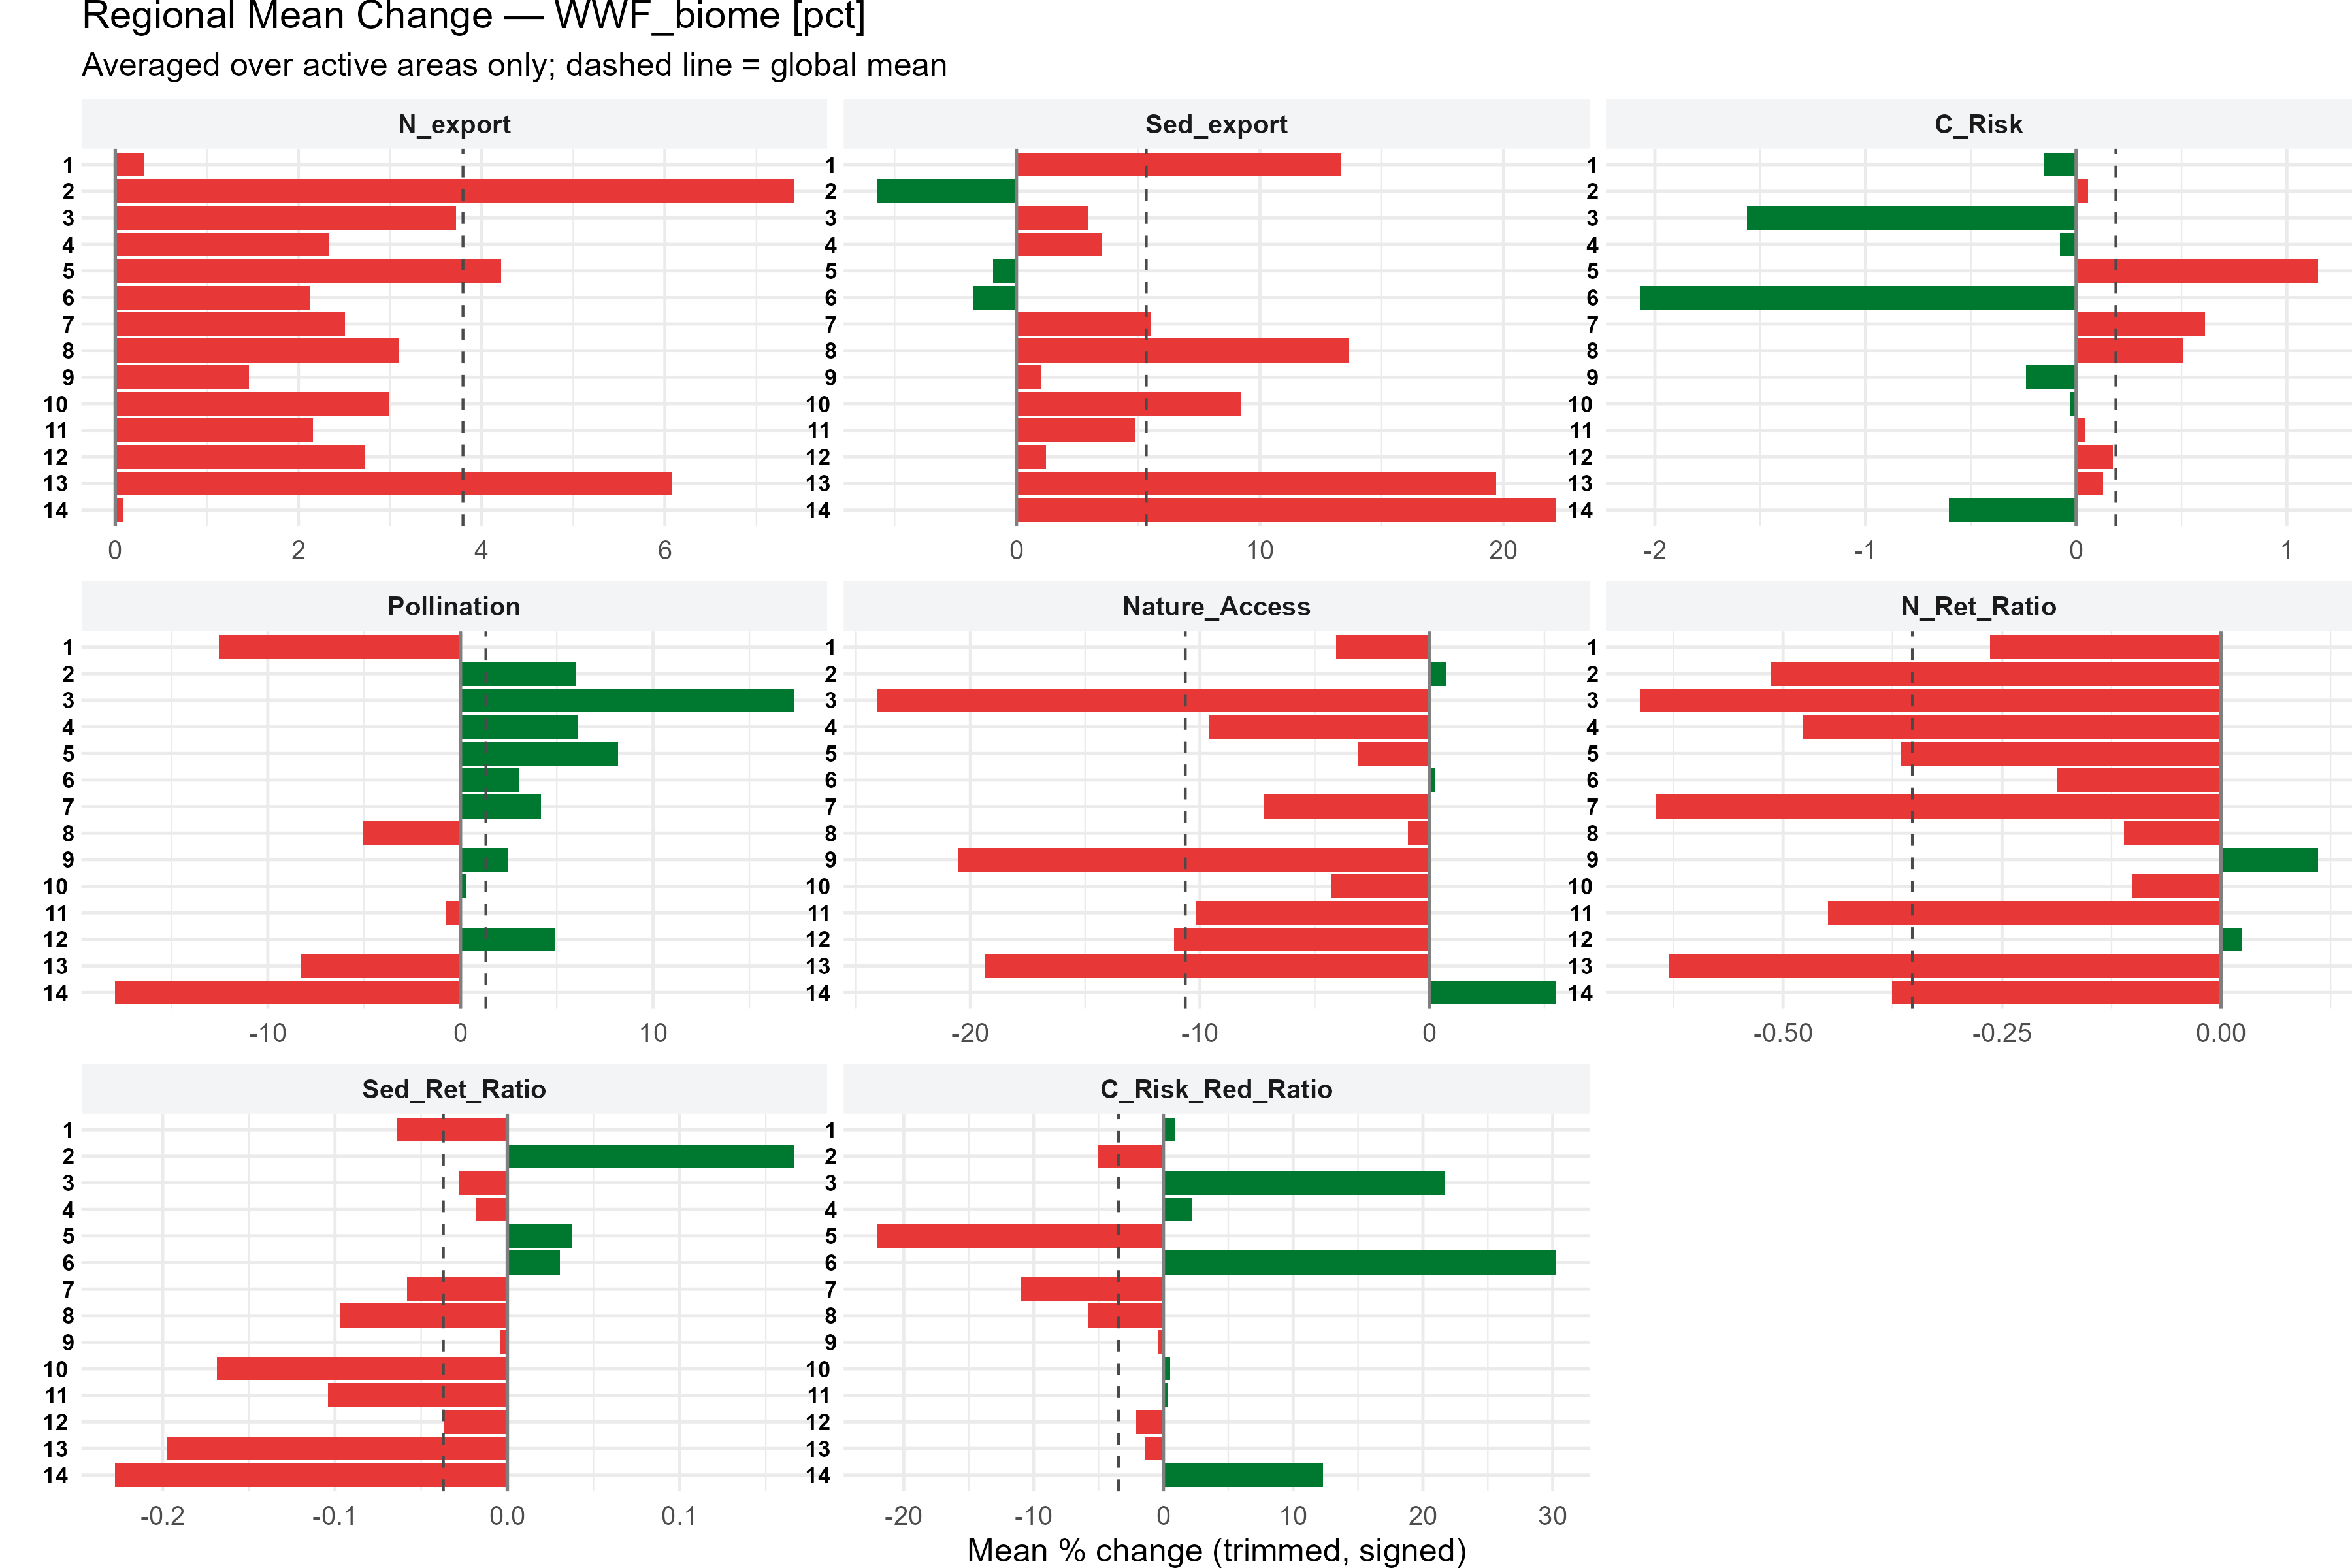
\includegraphics[keepaspectratio]{../outputs/plots/signed_bars/bars_signed_wwf_biome_pct.png}}

\section{Hotspot boxplots}\label{hotspot-boxplots}

Summarize hotspot distributions by group using saved PNGs; skip
computation if group columns are absent. Helper
\texttt{run\_hotspot\_boxplots\_by()} now lives in
\texttt{R/hotspot\_violins.R}, so we just call it from this report.

Outputs: PNGs are written to
\texttt{outputs/plots/\{abs\textbar{}pct\}/\textless{}group\_col\textgreater{}/boxplots\_*.png}
and mirrored into \texttt{outputs/plots/latest/boxplots/} for embedding.

\begin{verbatim}
==> Boxplots by: income_grp
\end{verbatim}

\begin{verbatim}
==> Boxplots by: region_wb
\end{verbatim}

\begin{verbatim}
==> Boxplots by: WWF_biome
\end{verbatim}

\pandocbounded{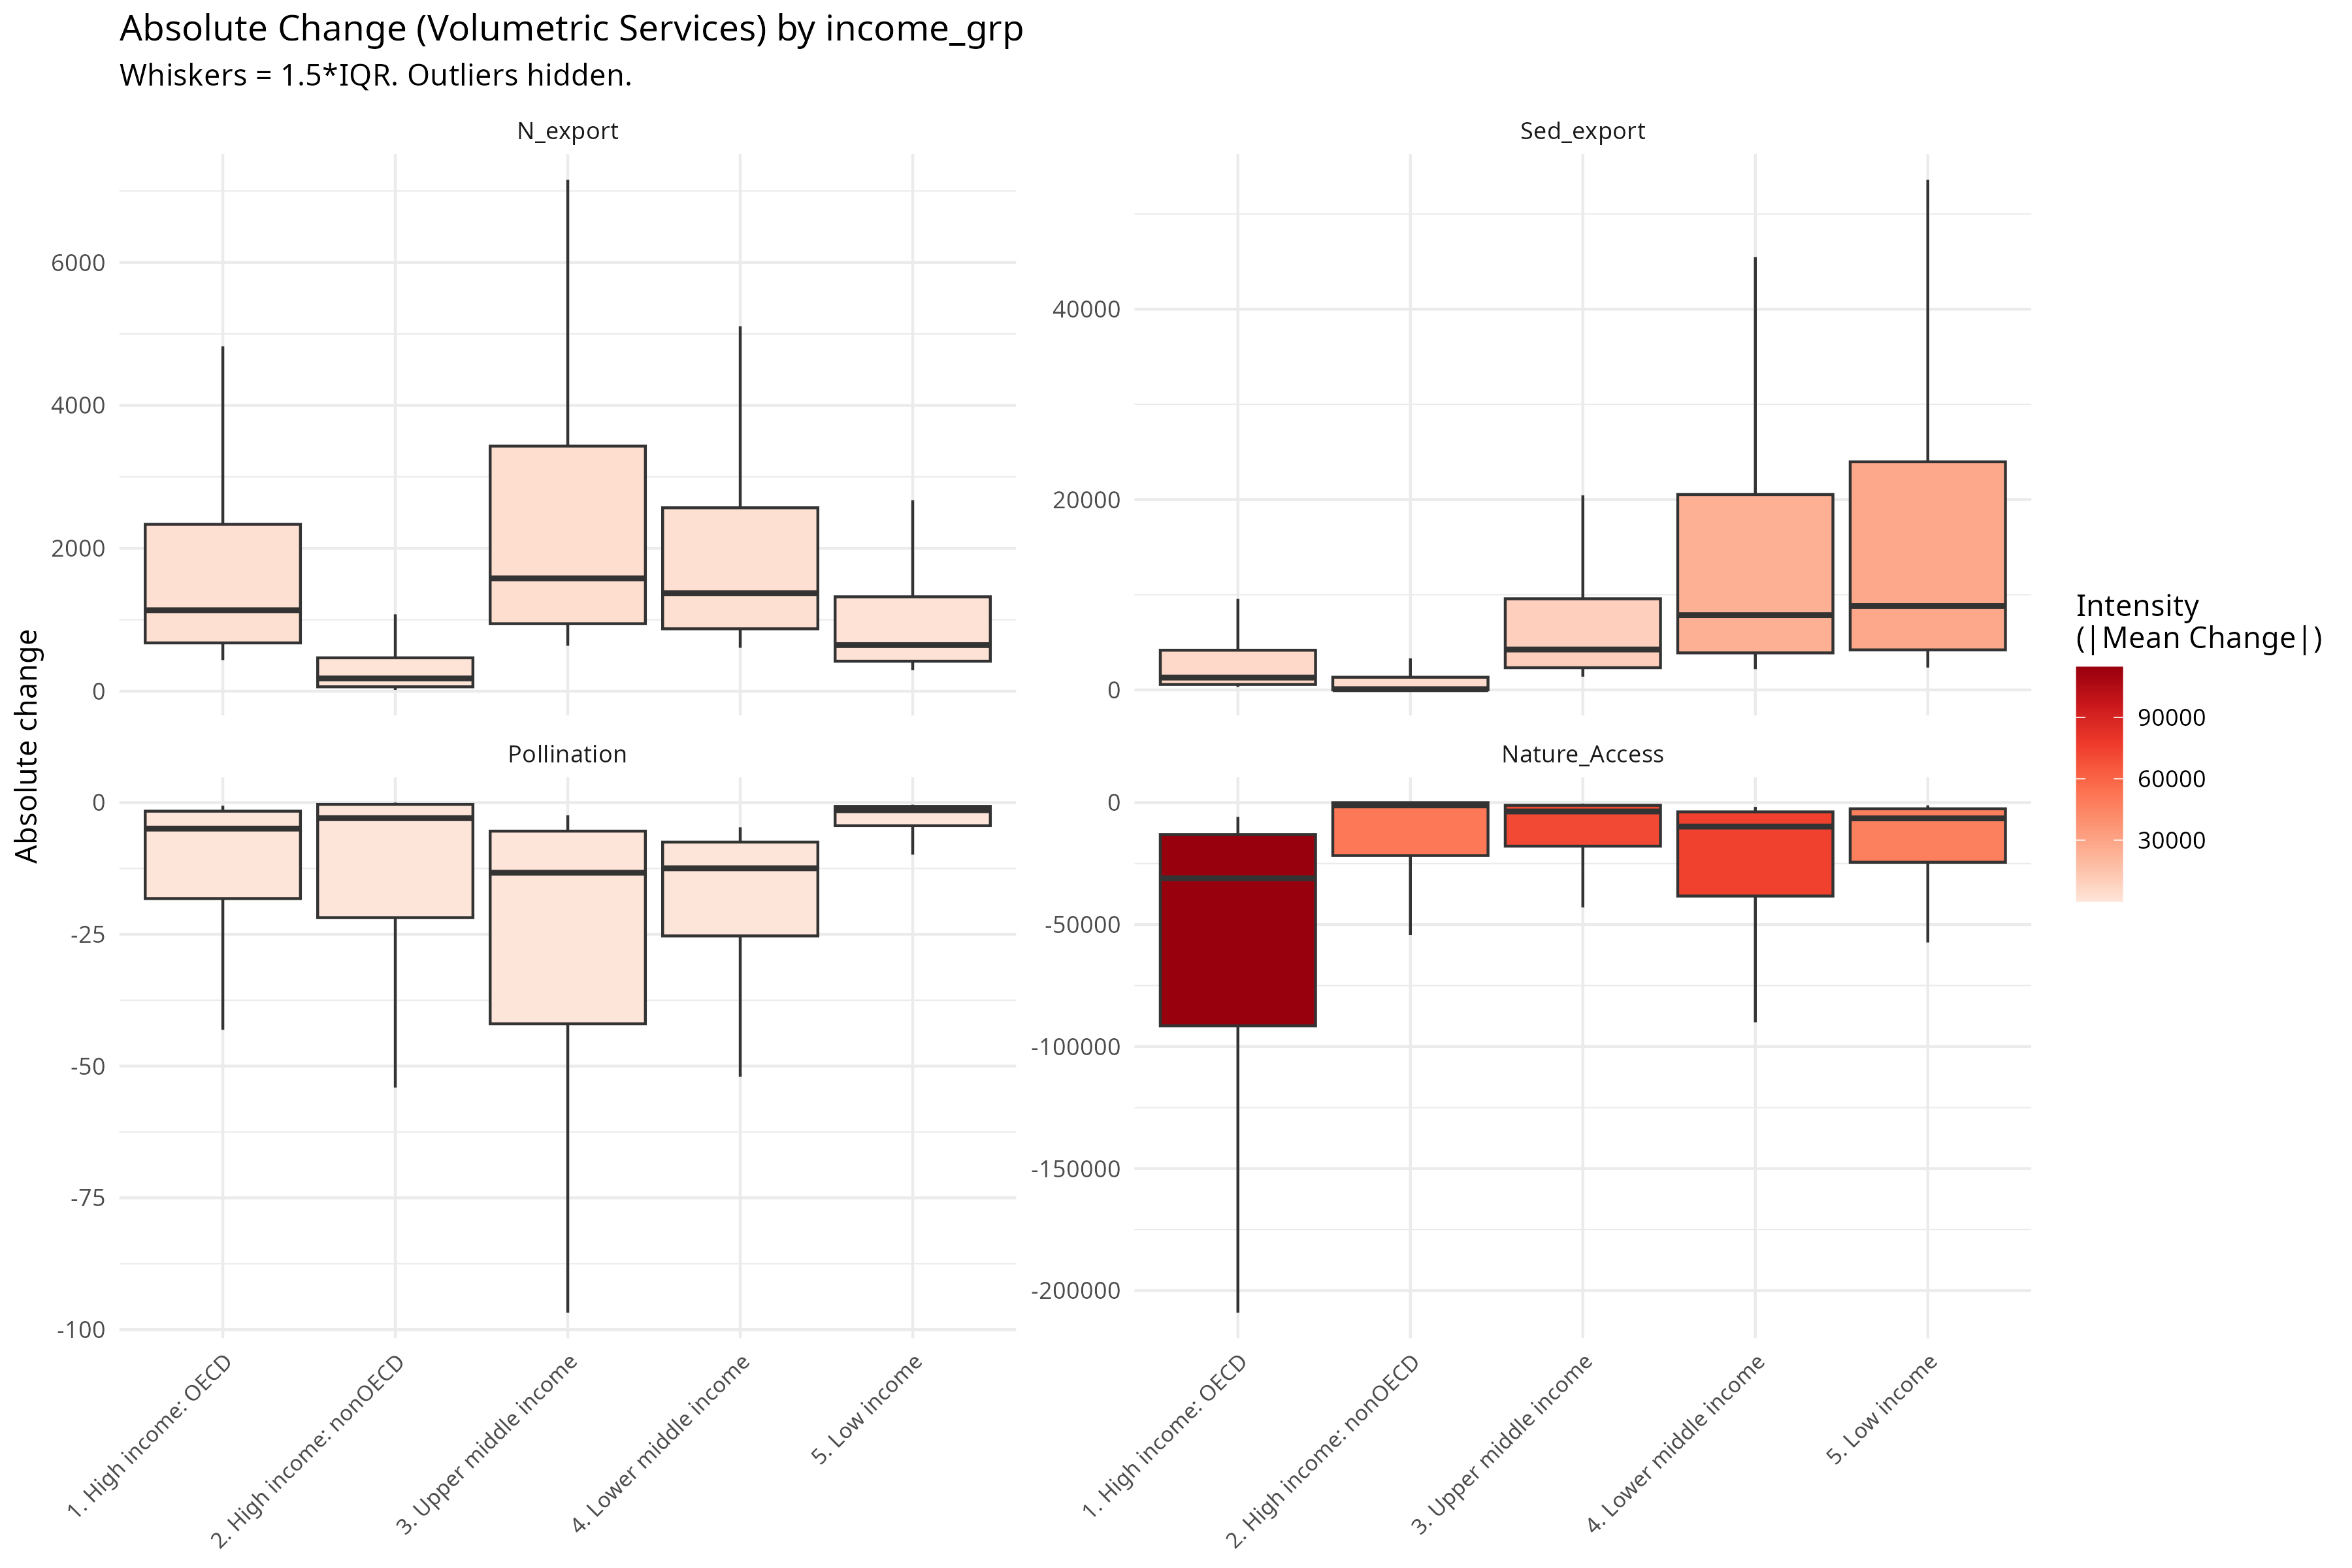
\includegraphics[keepaspectratio]{../outputs/plots/abs/income_grp/boxplots_income_grp_abs_volumetric.png}}

\pandocbounded{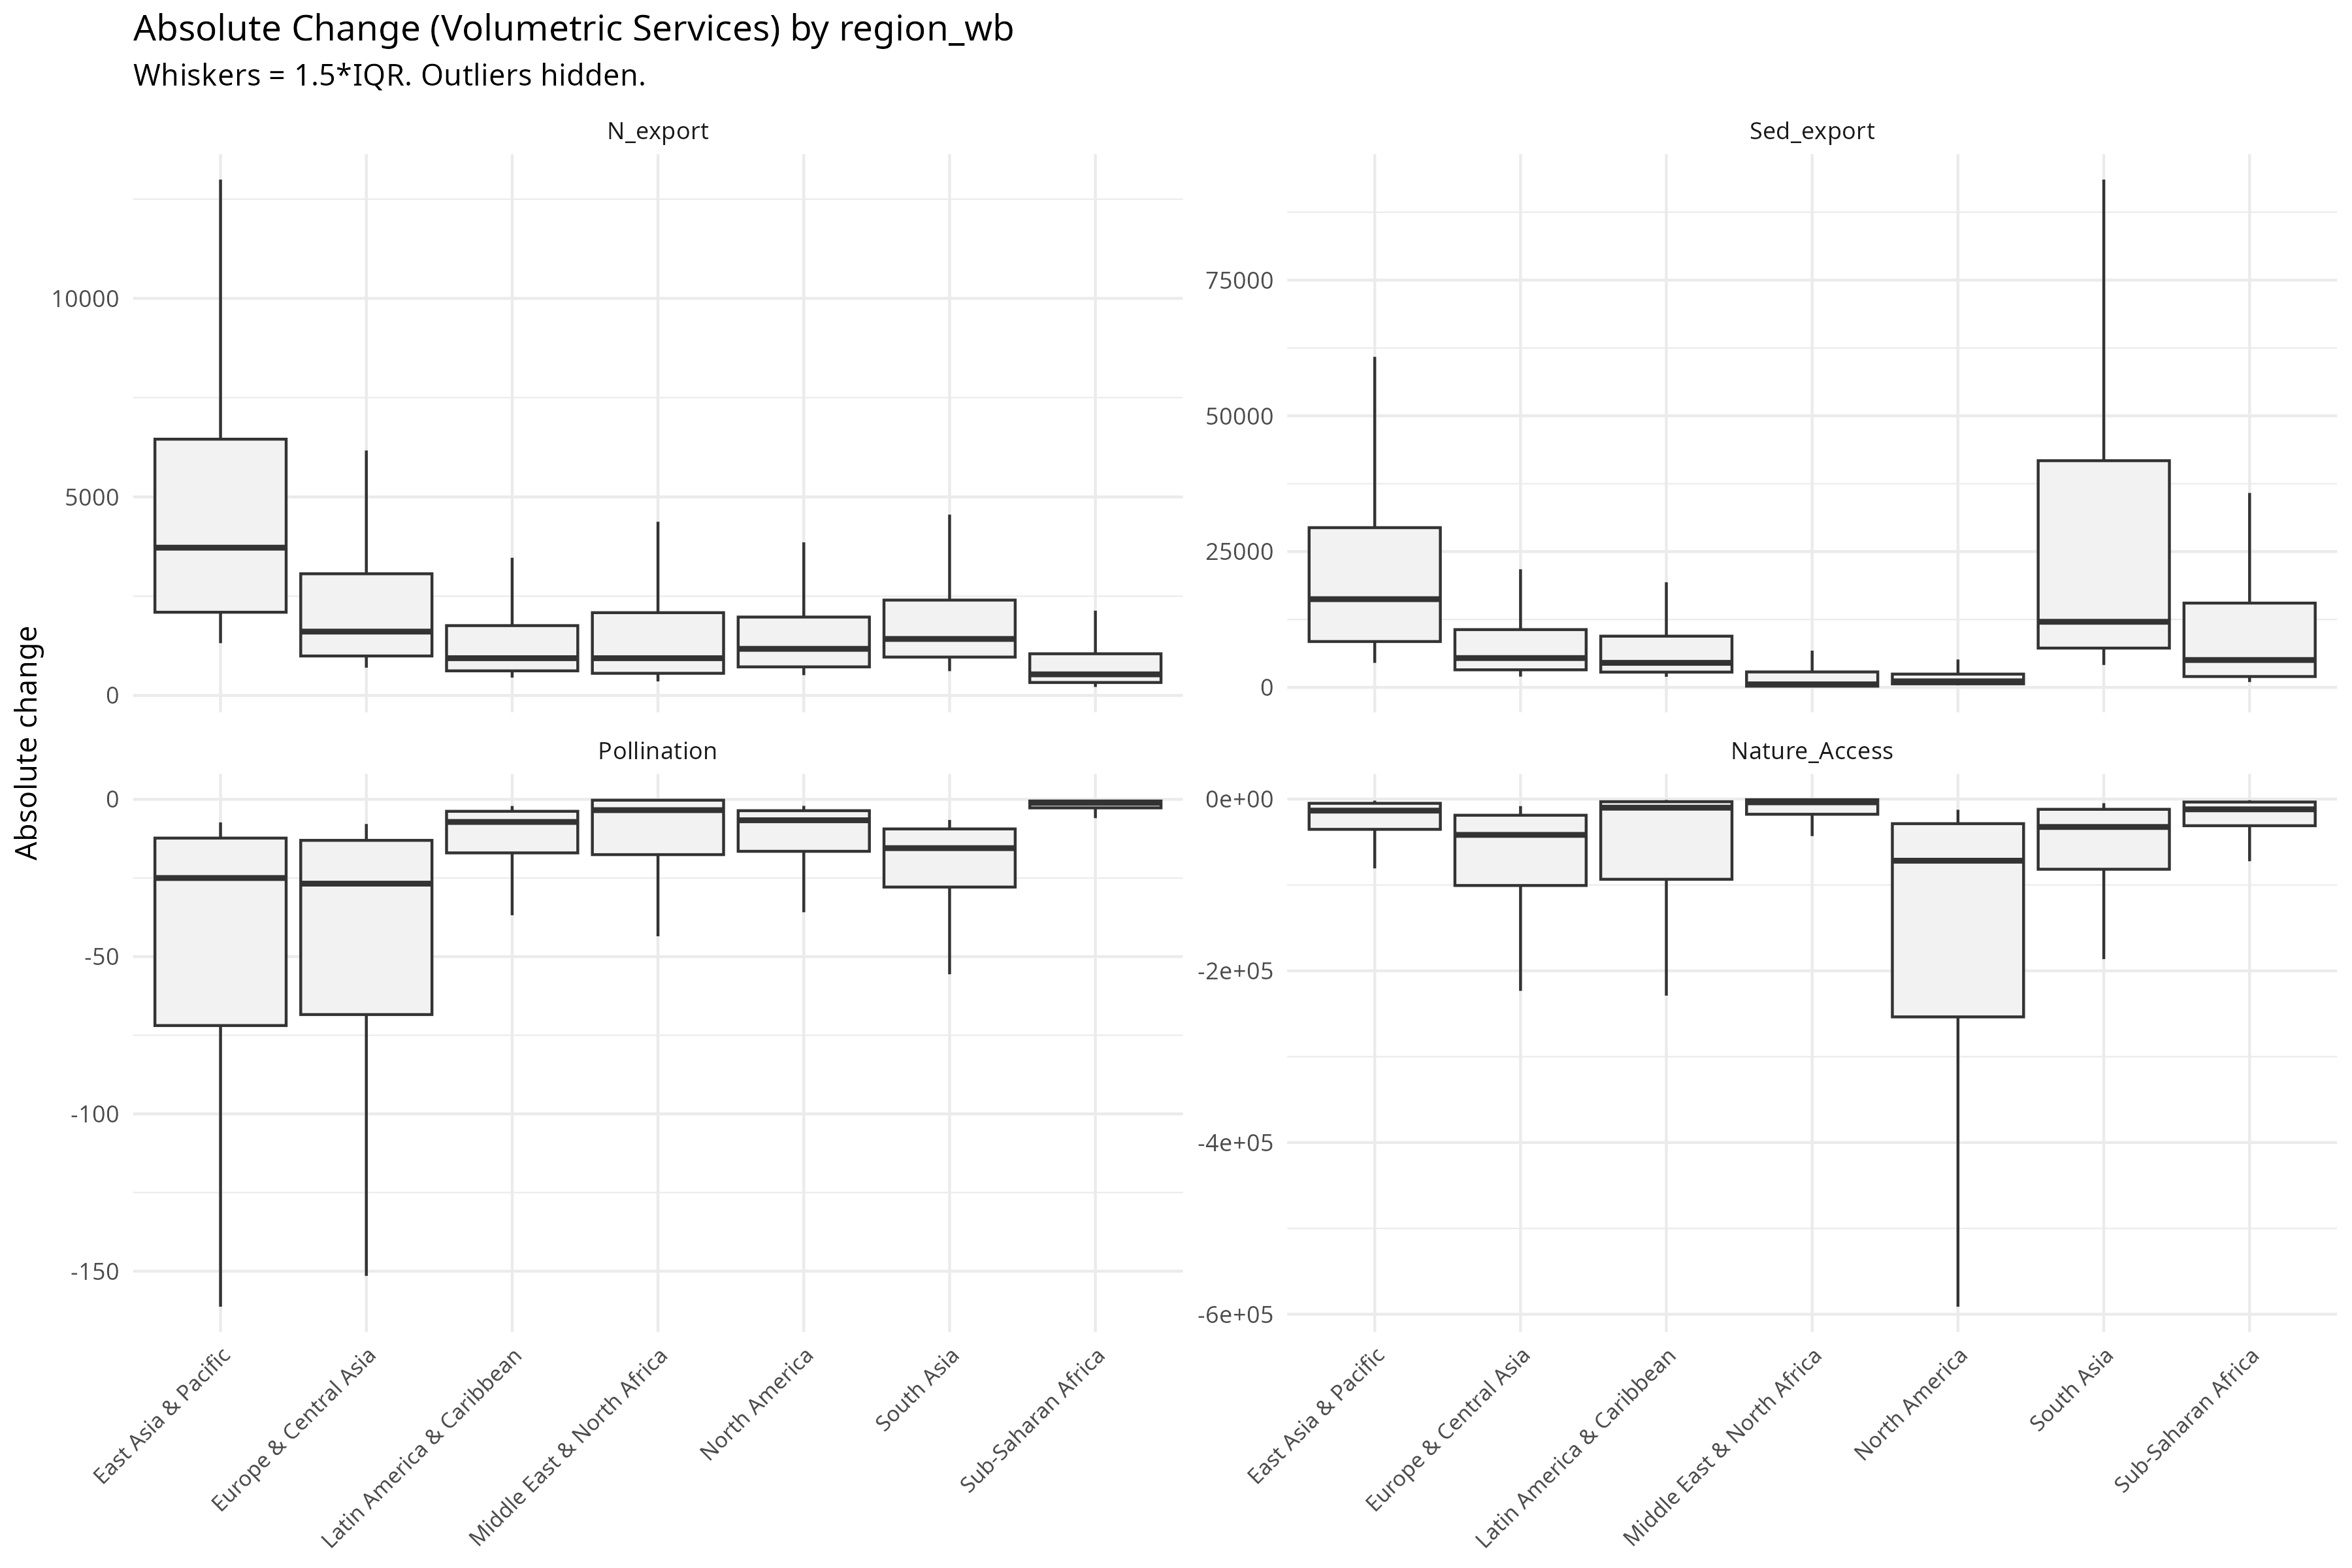
\includegraphics[keepaspectratio]{../outputs/plots/abs/region_wb/boxplots_region_wb_abs_volumetric.png}}

\pandocbounded{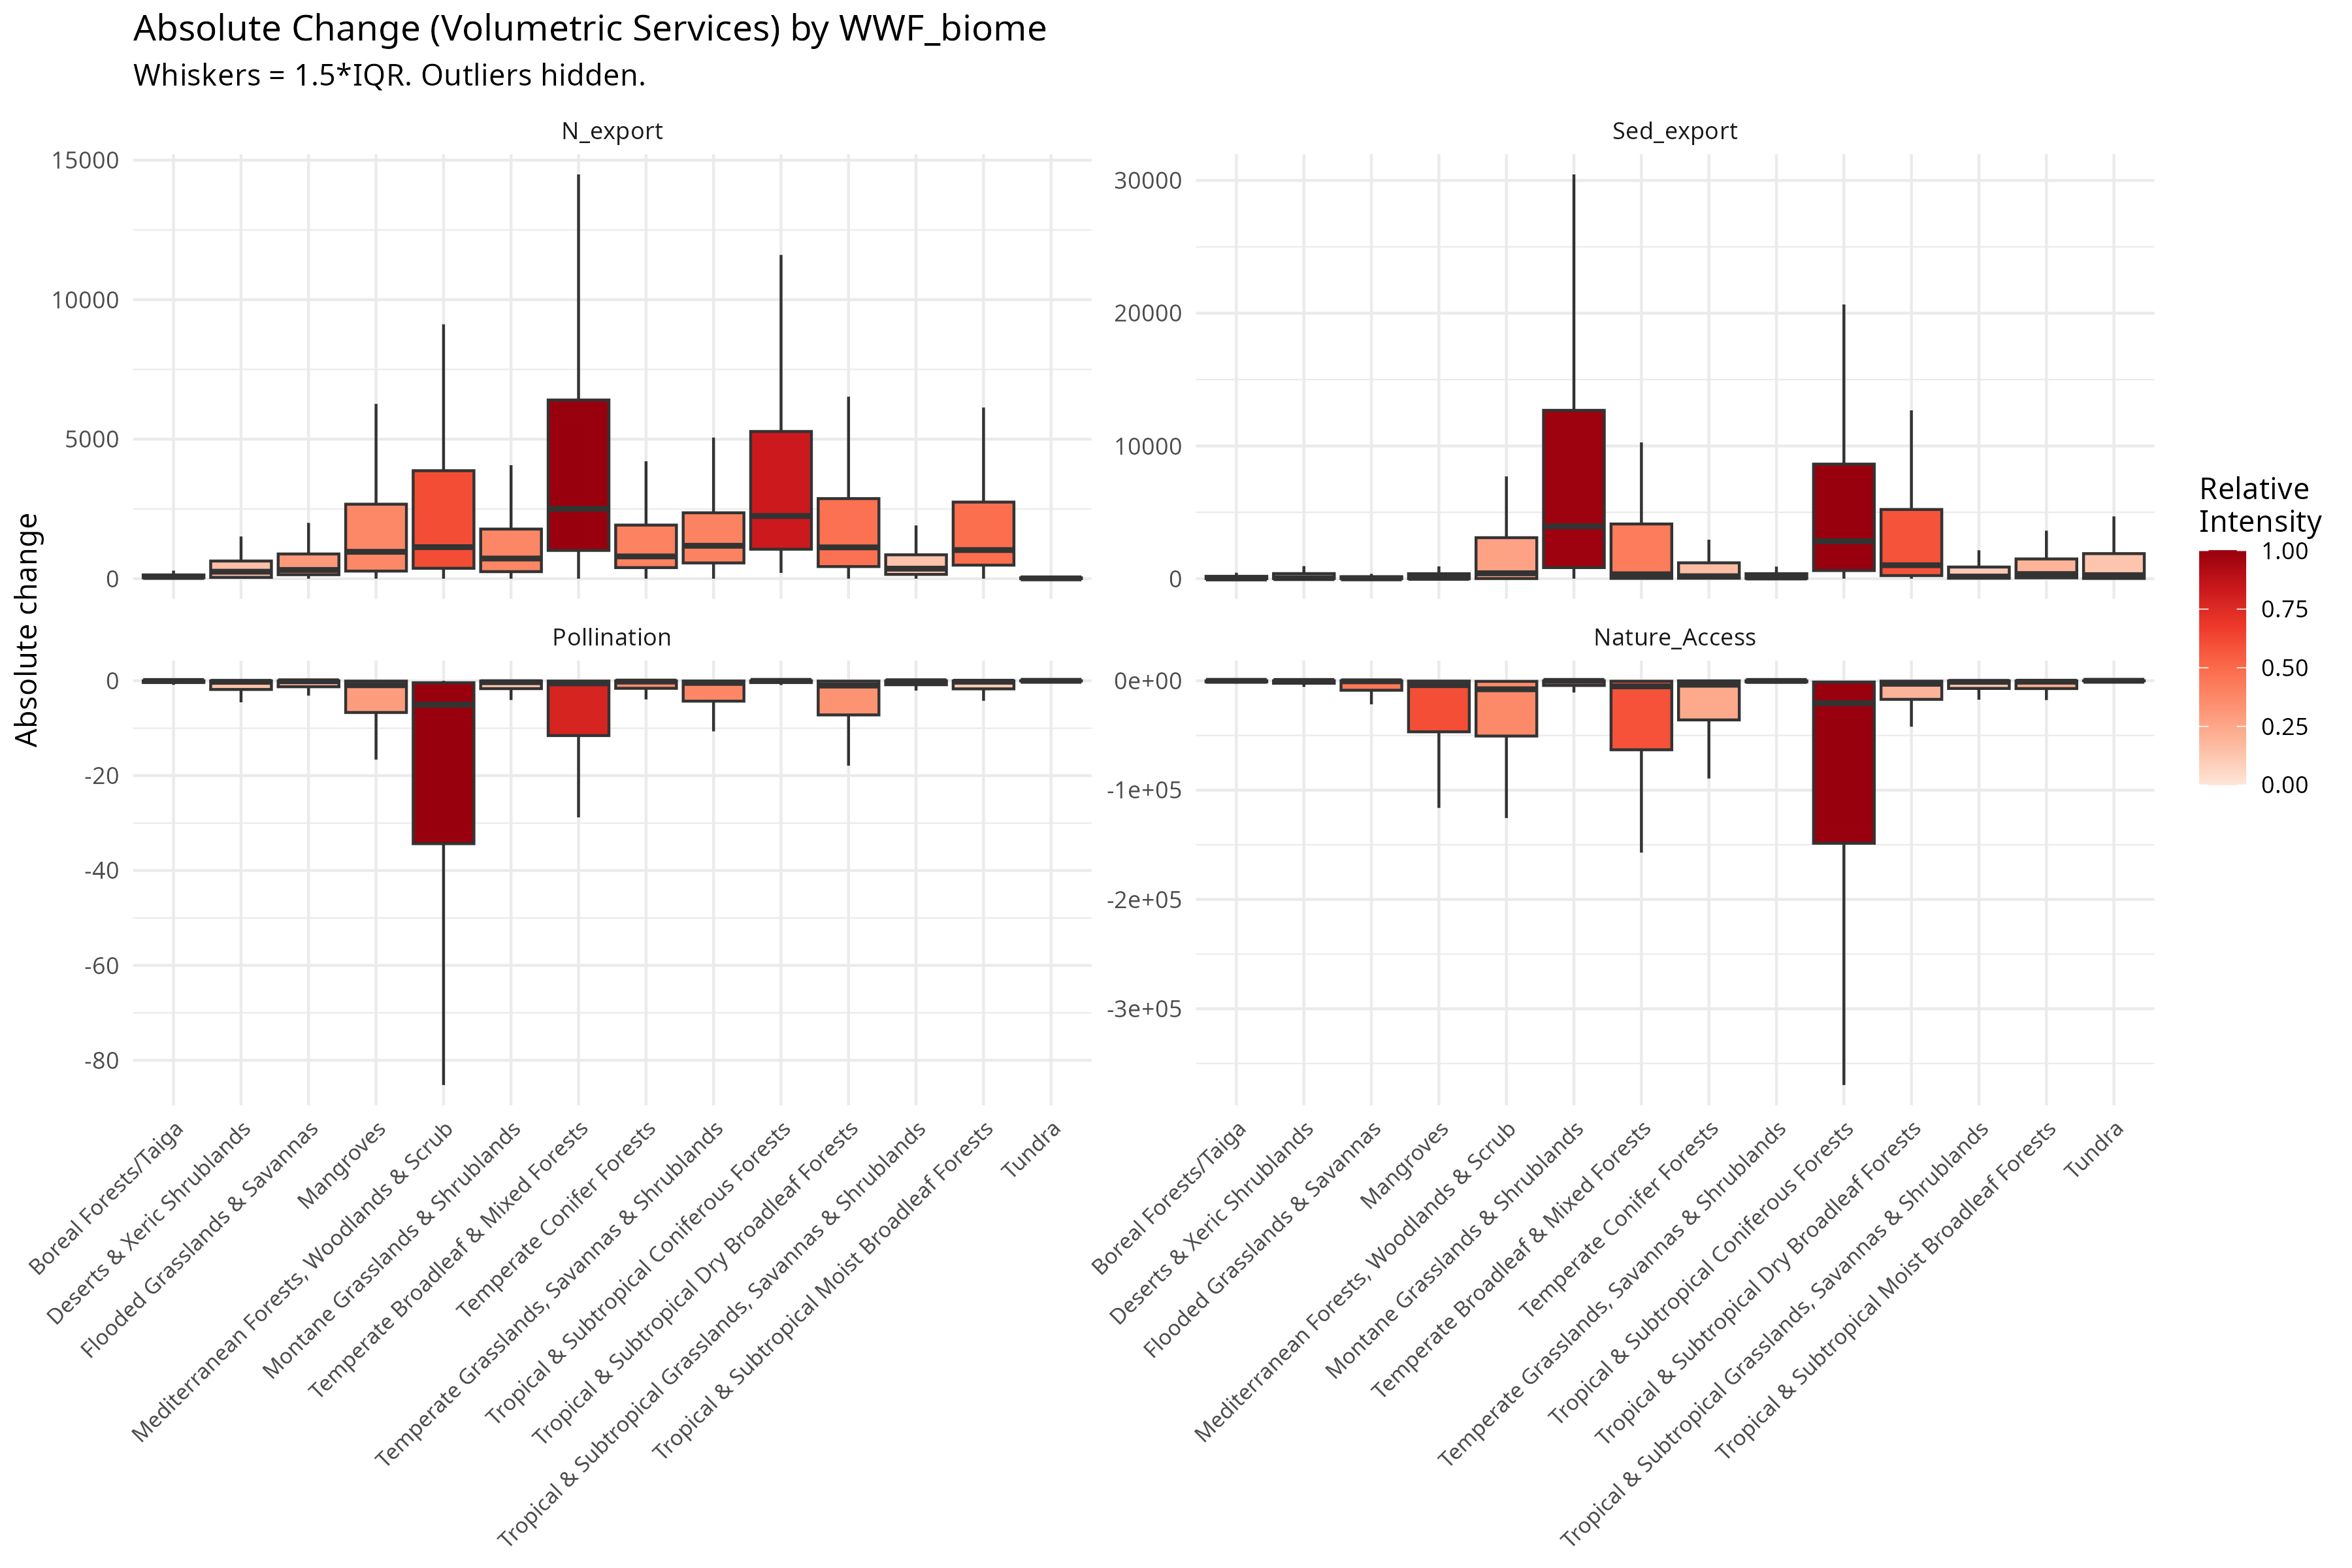
\includegraphics[keepaspectratio]{../outputs/plots/abs/wwf_biome/boxplots_wwf_biome_abs_volumetric.png}}

\pandocbounded{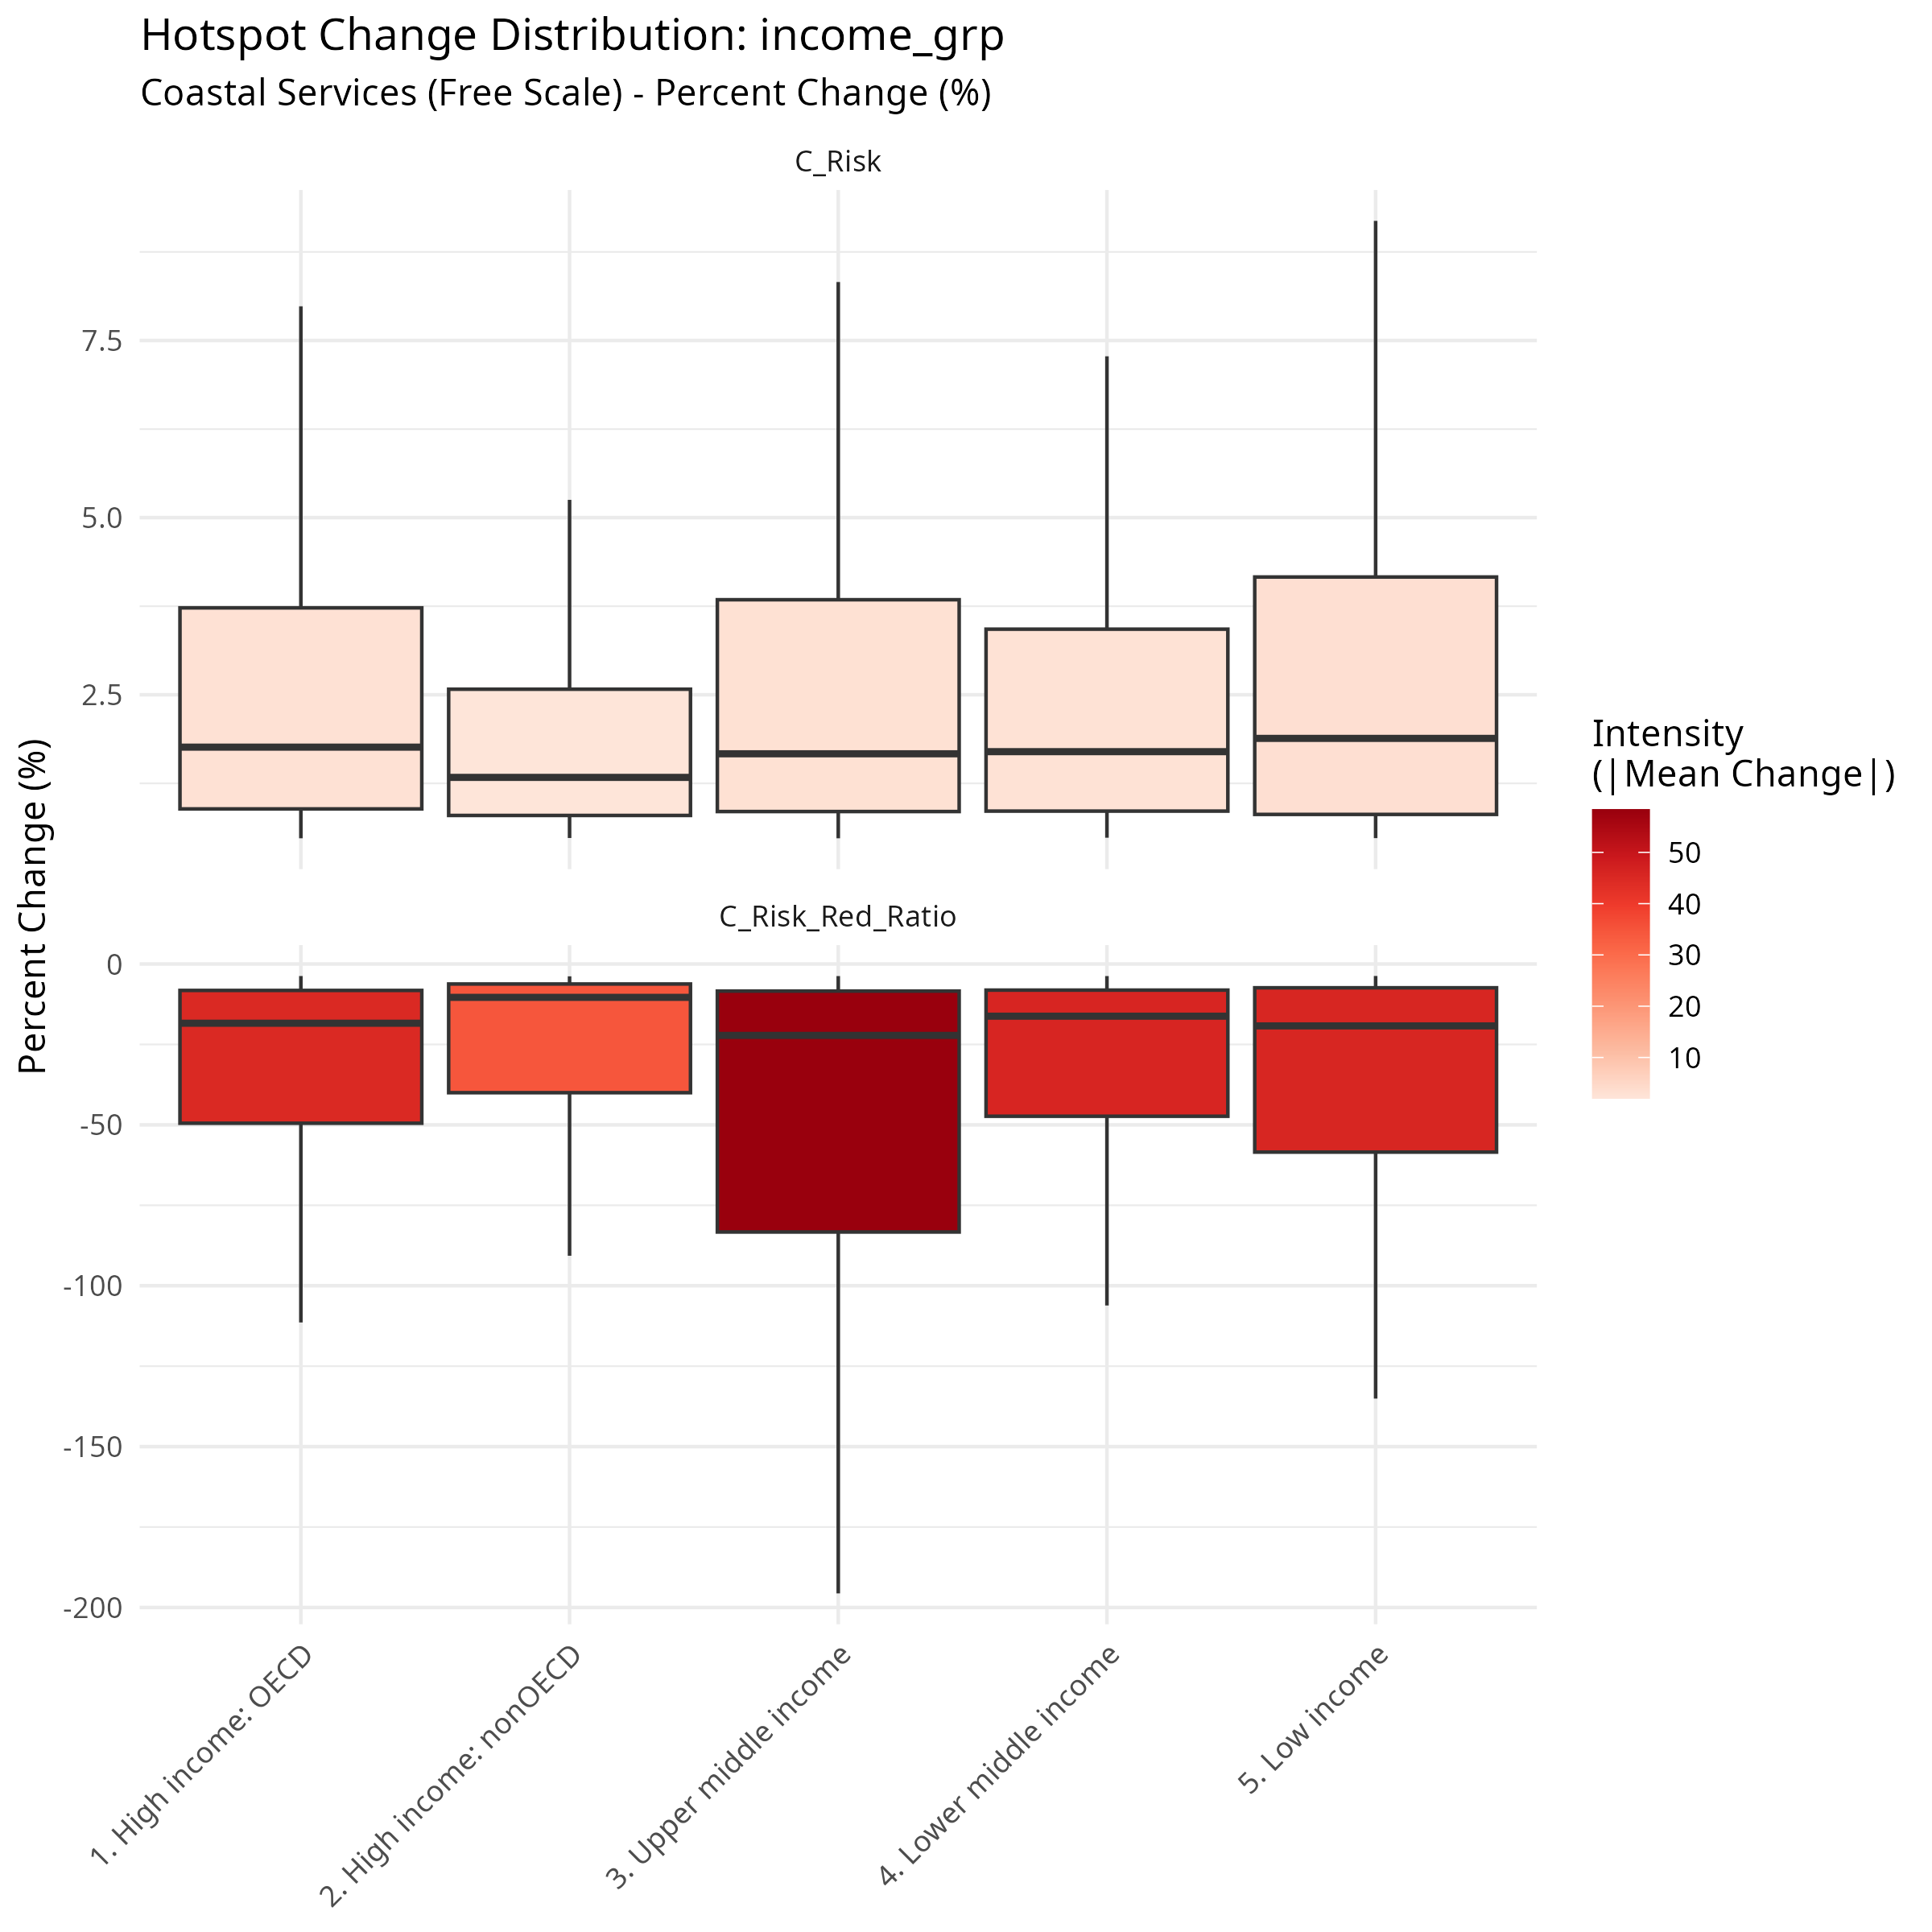
\includegraphics[keepaspectratio]{../outputs/plots/coastal/income_grp/boxplots_income_grp_pct_coastal.png}}

\pandocbounded{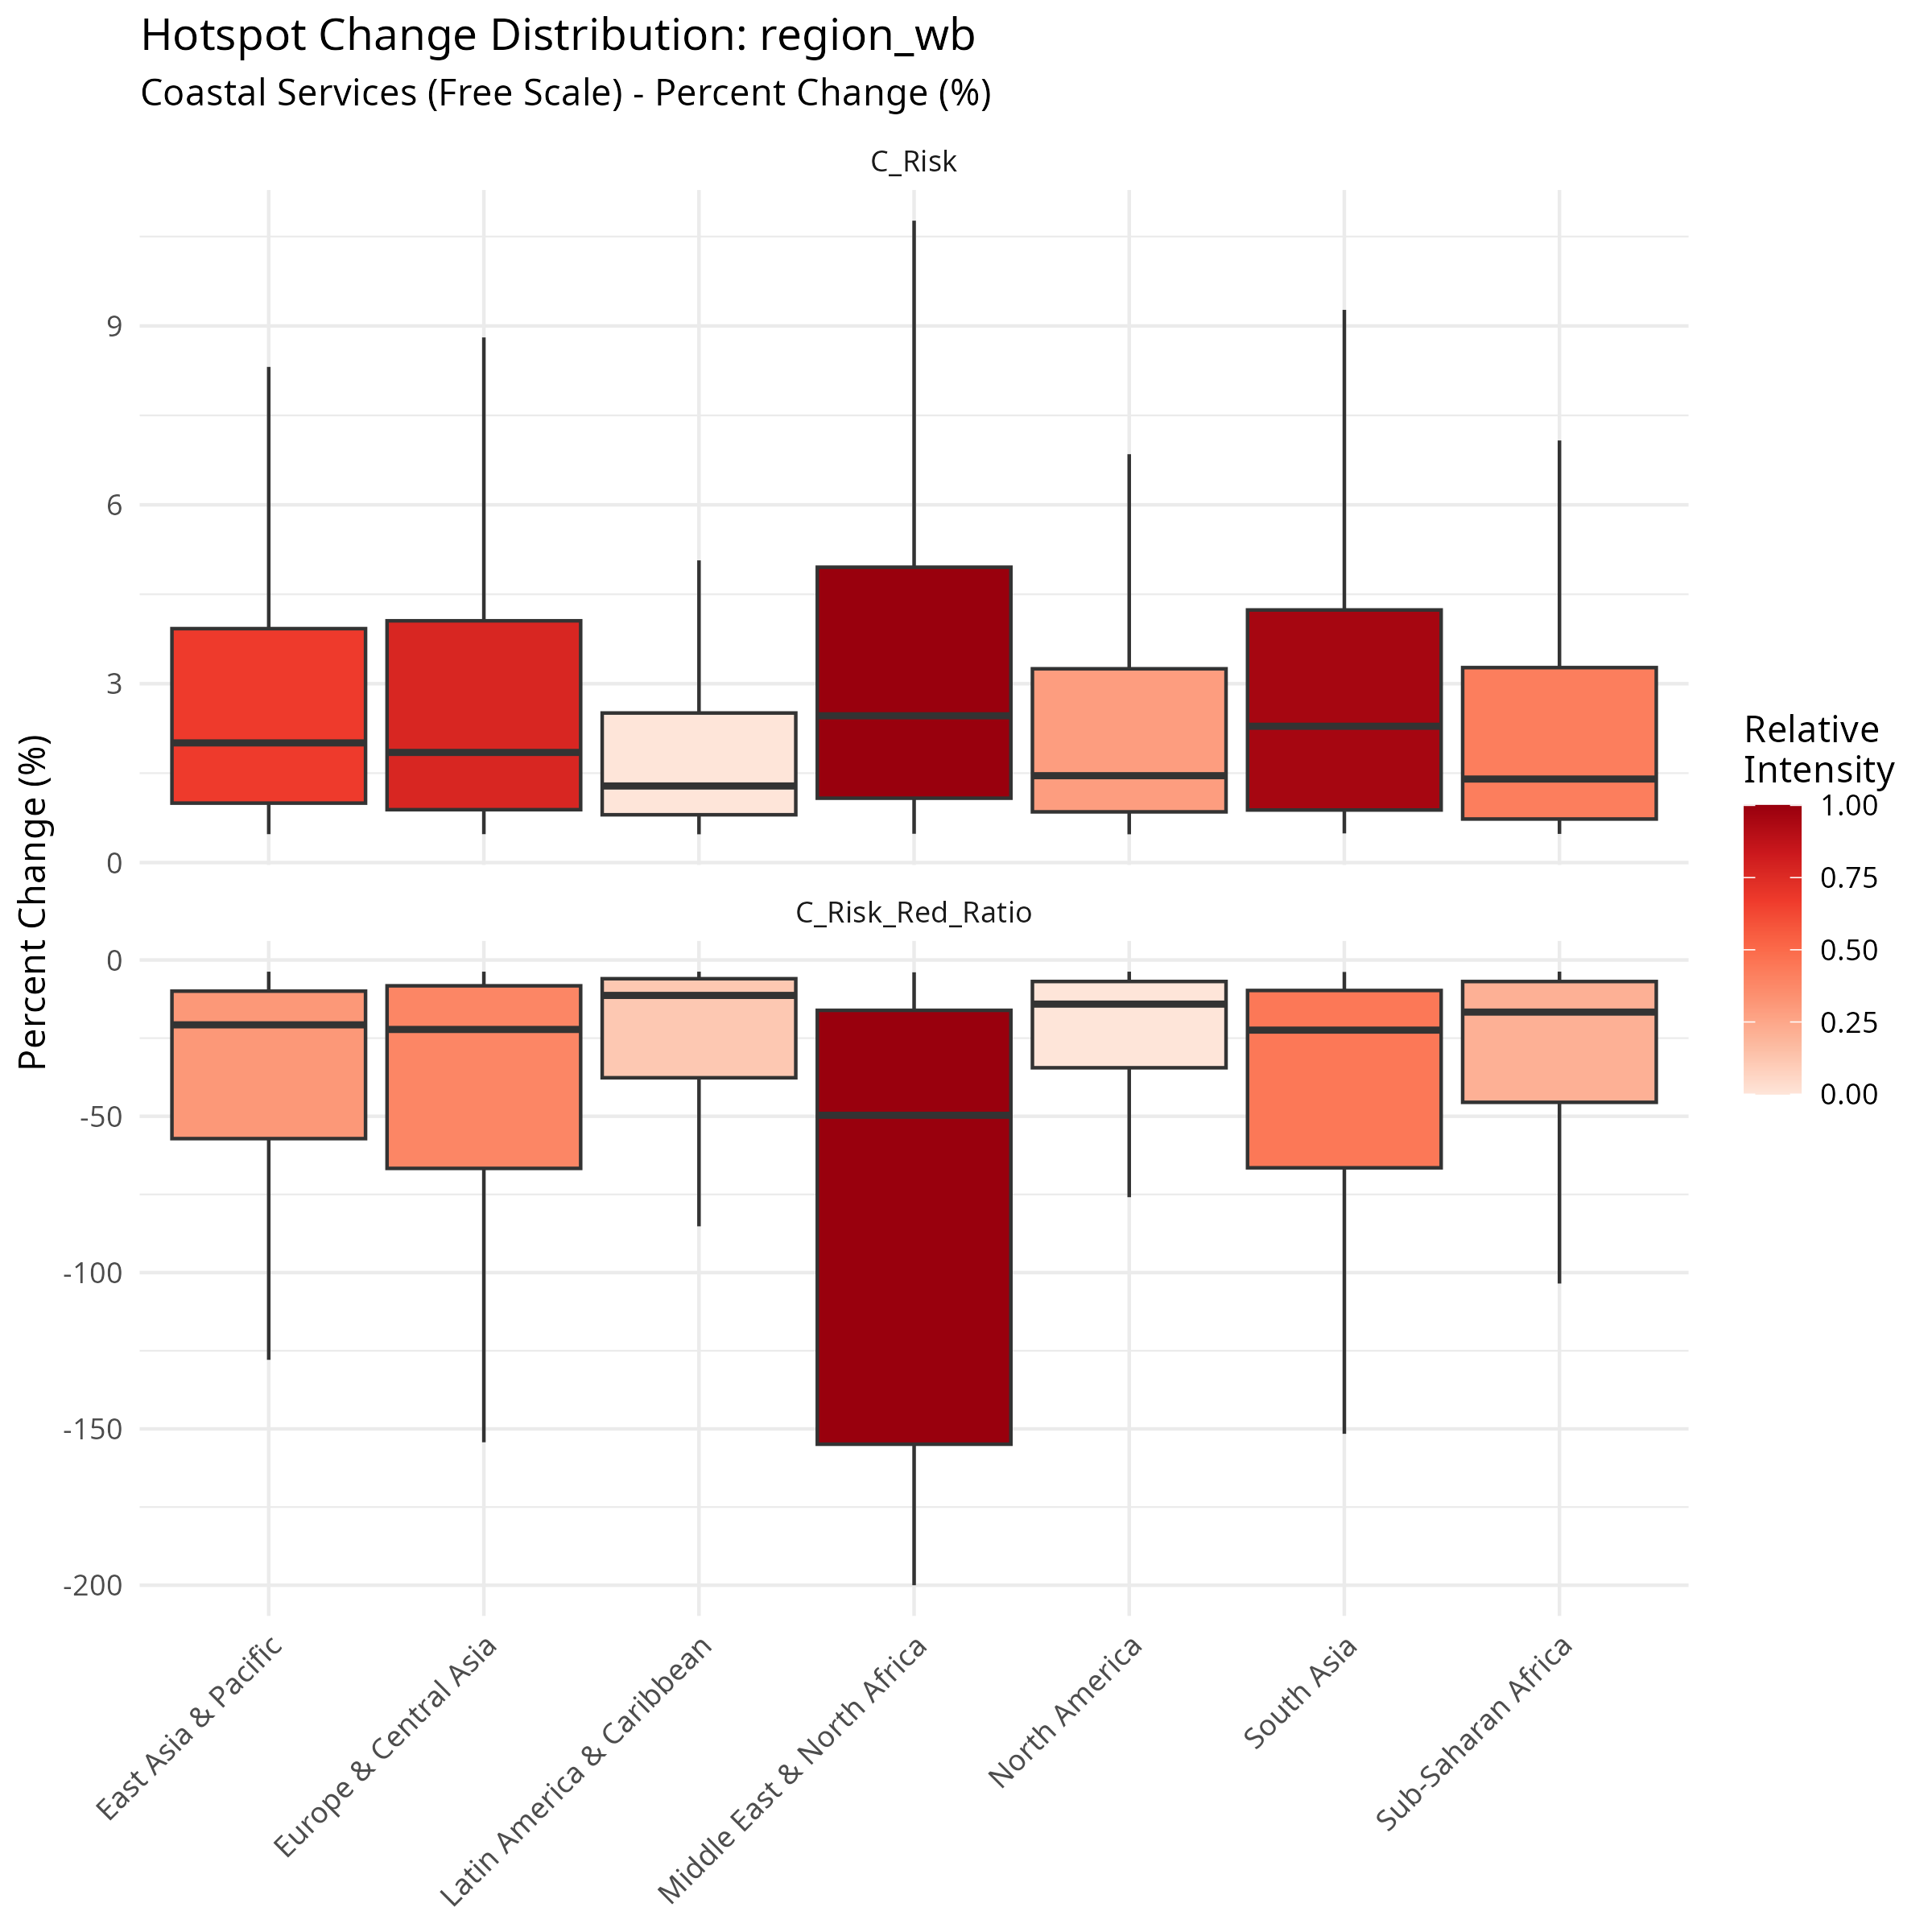
\includegraphics[keepaspectratio]{../outputs/plots/coastal/region_wb/boxplots_region_wb_pct_coastal.png}}

\pandocbounded{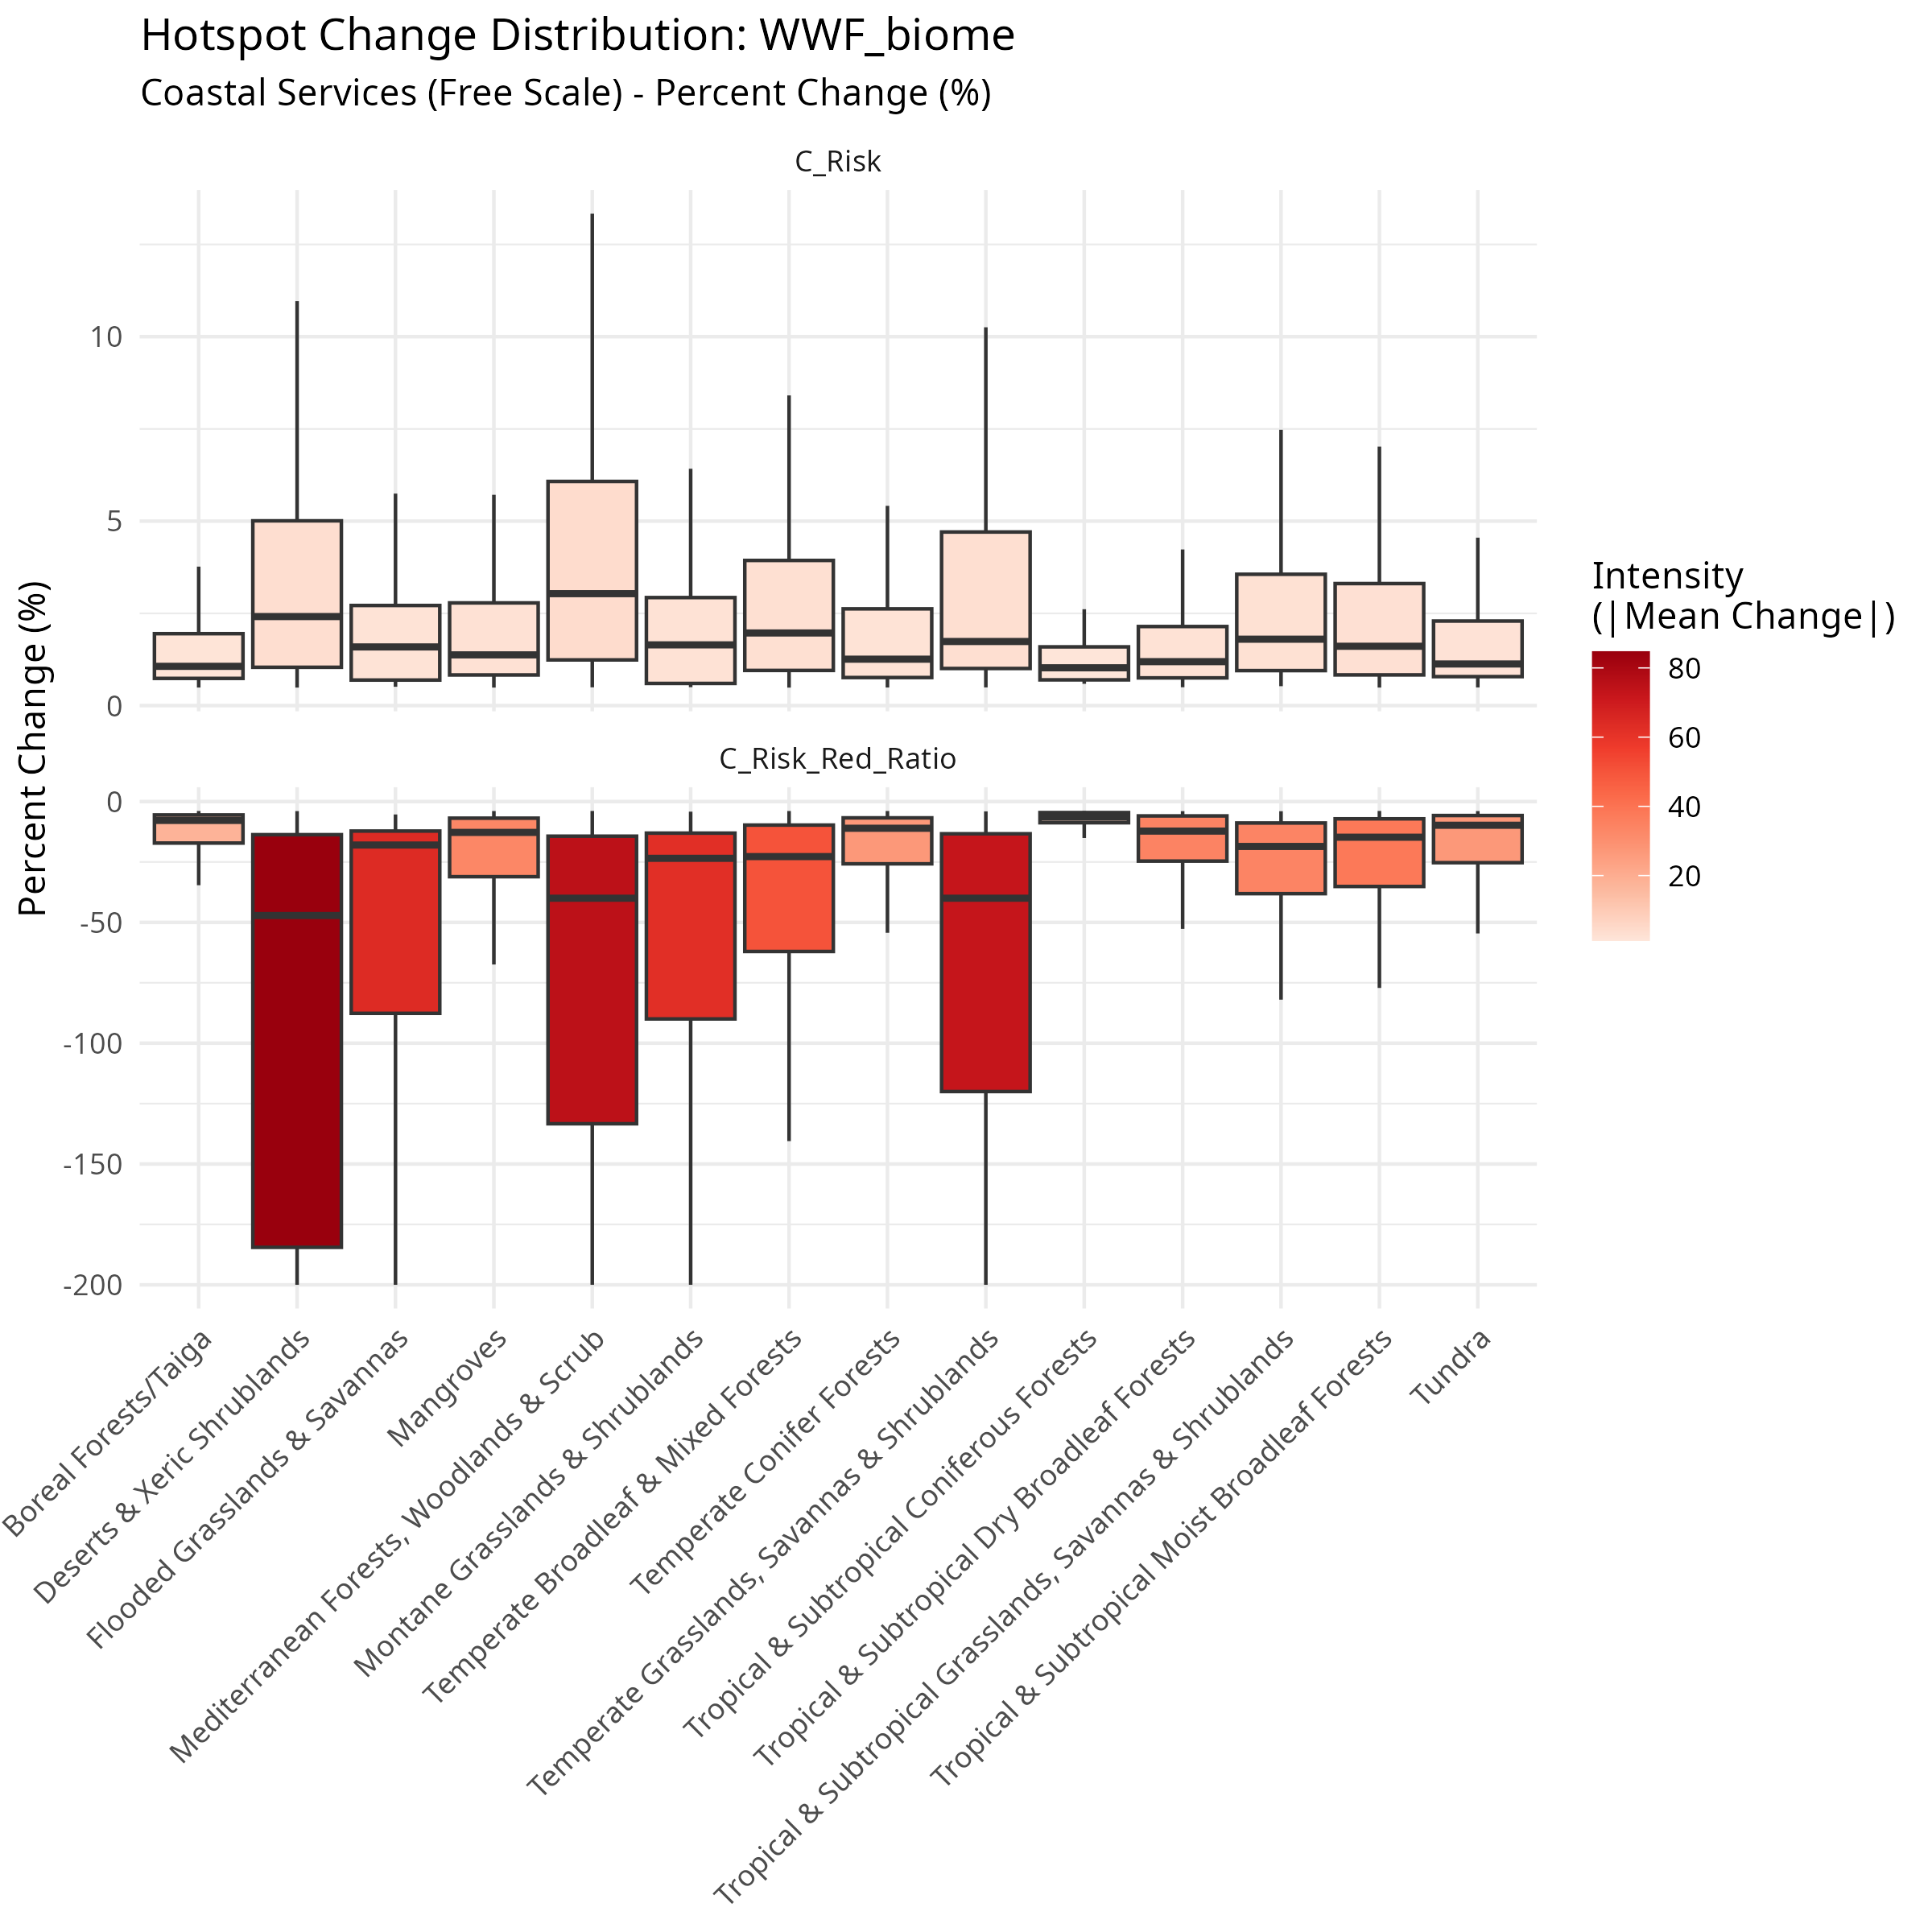
\includegraphics[keepaspectratio]{../outputs/plots/coastal/WWF_biome/boxplots_WWF_biome_pct_coastal.png}}

\pandocbounded{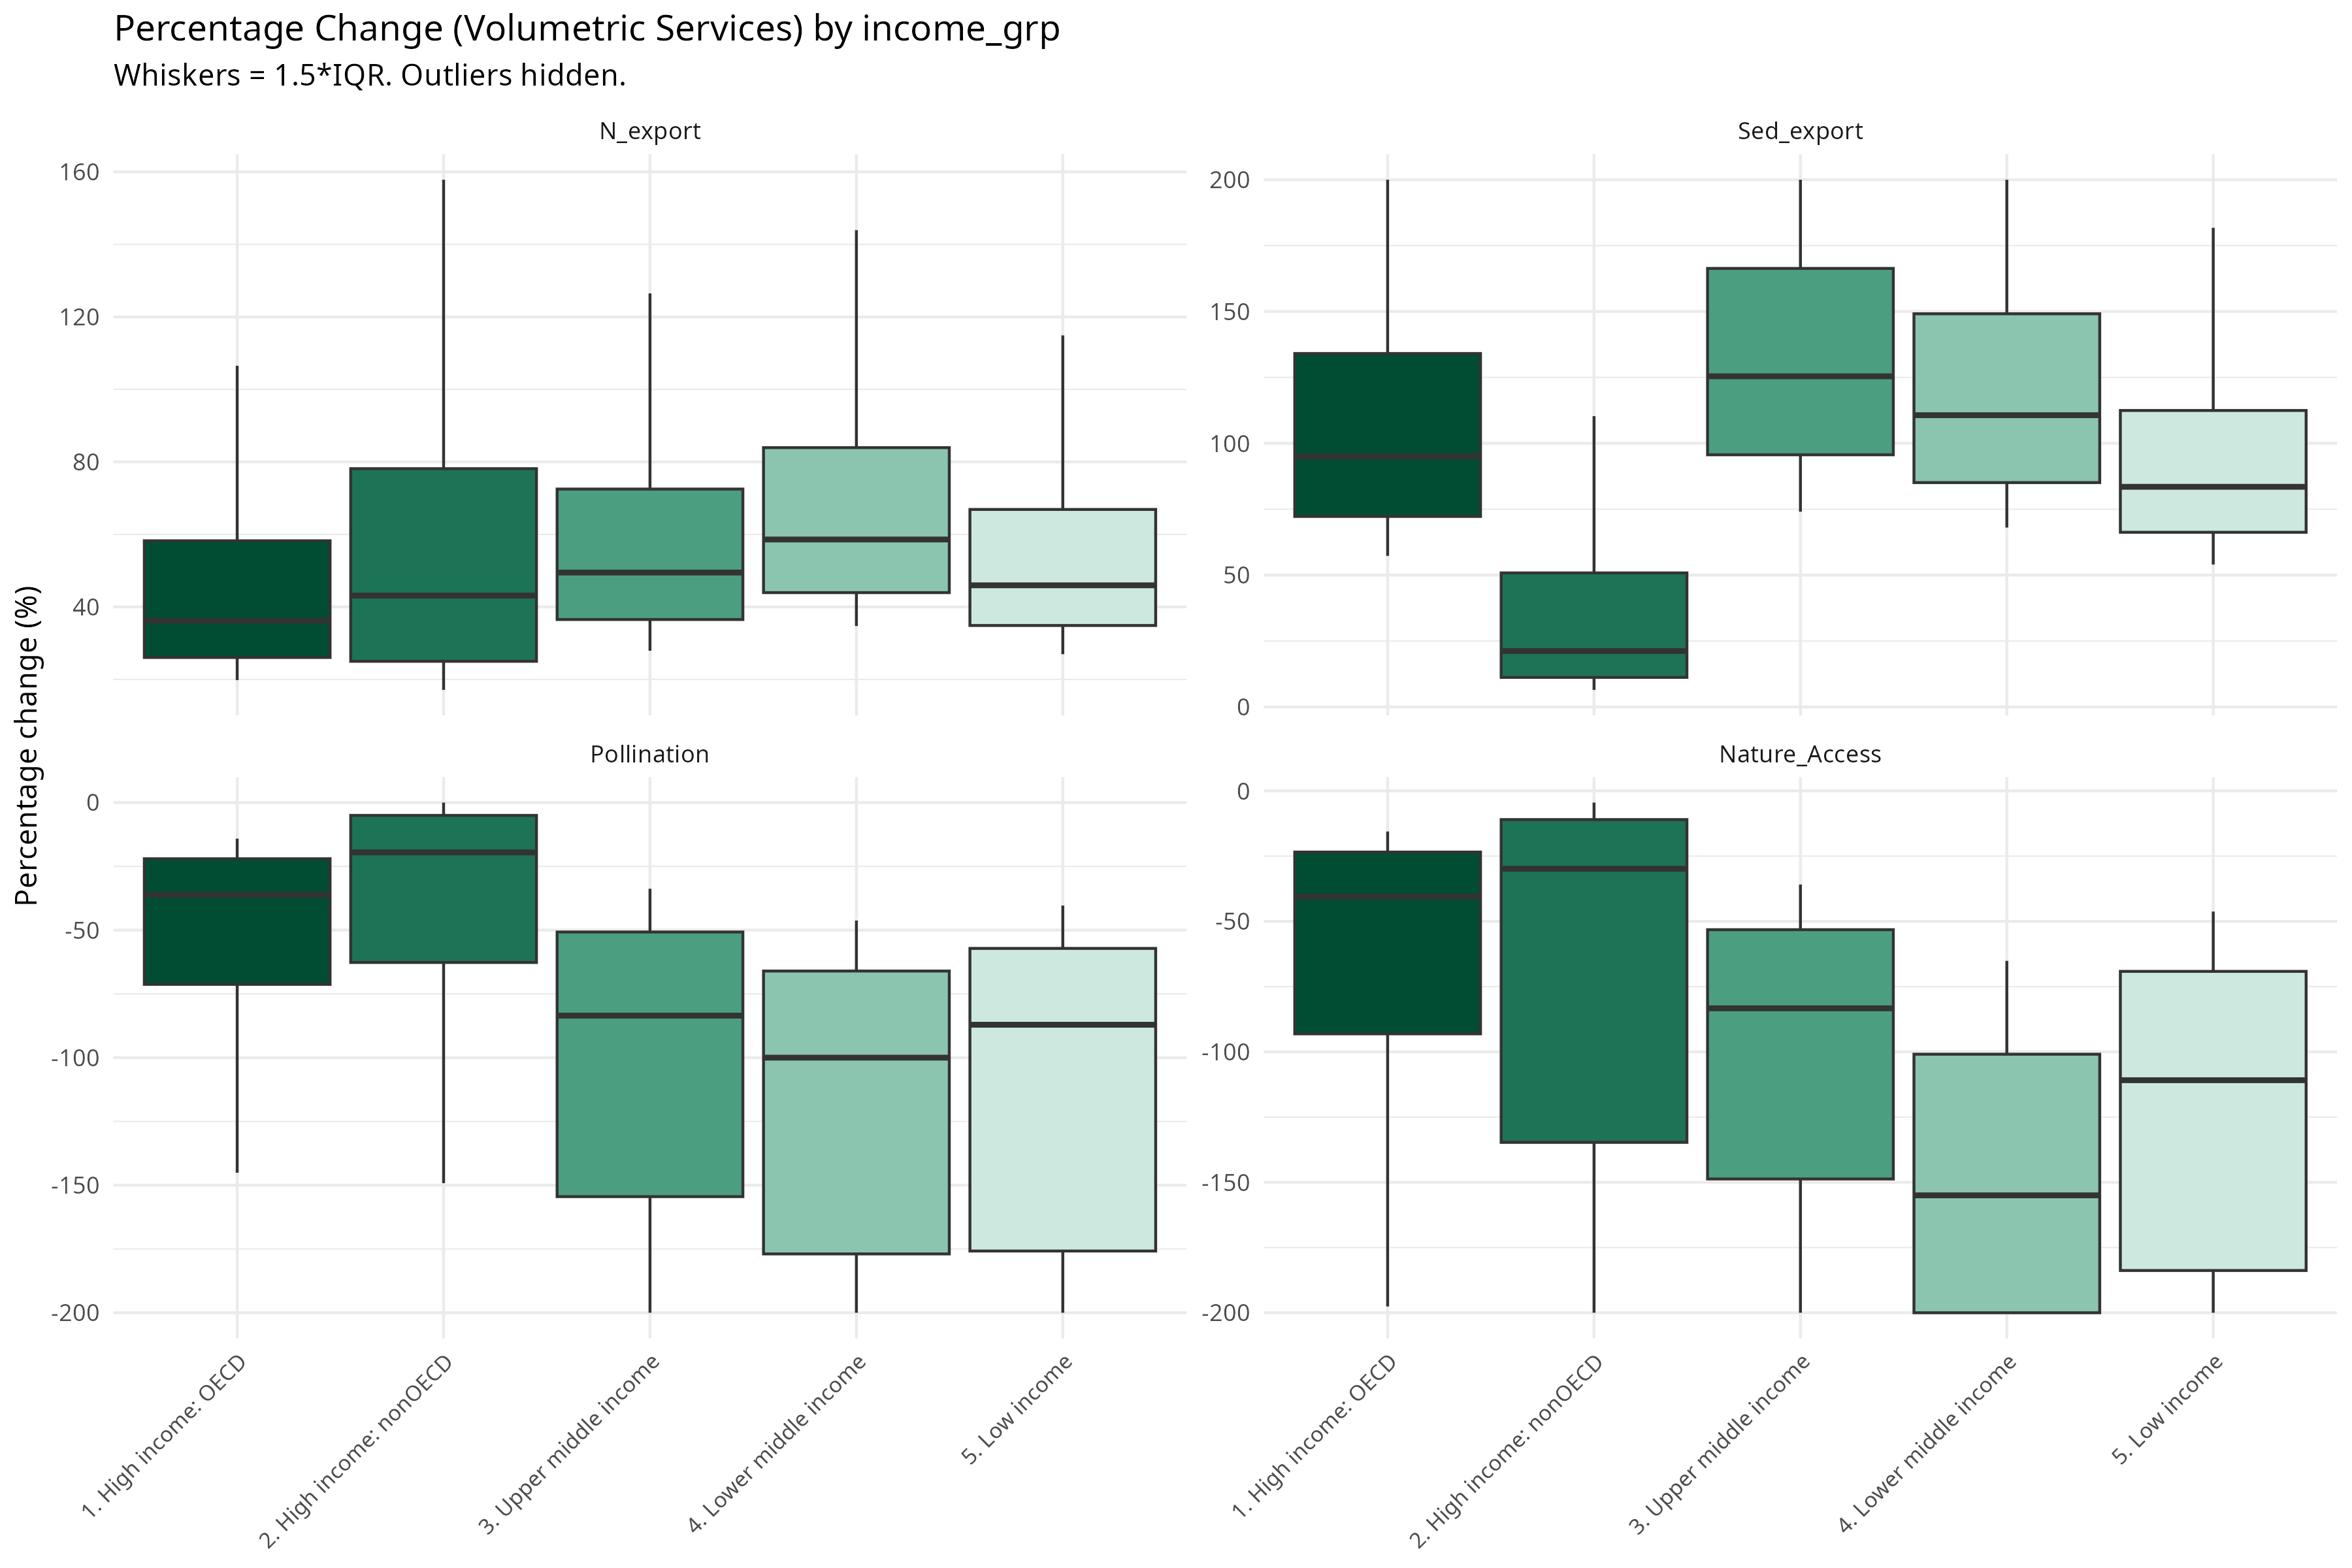
\includegraphics[keepaspectratio]{../outputs/plots/pct/income_grp/boxplots_income_grp_pct_volumetric.png}}

\pandocbounded{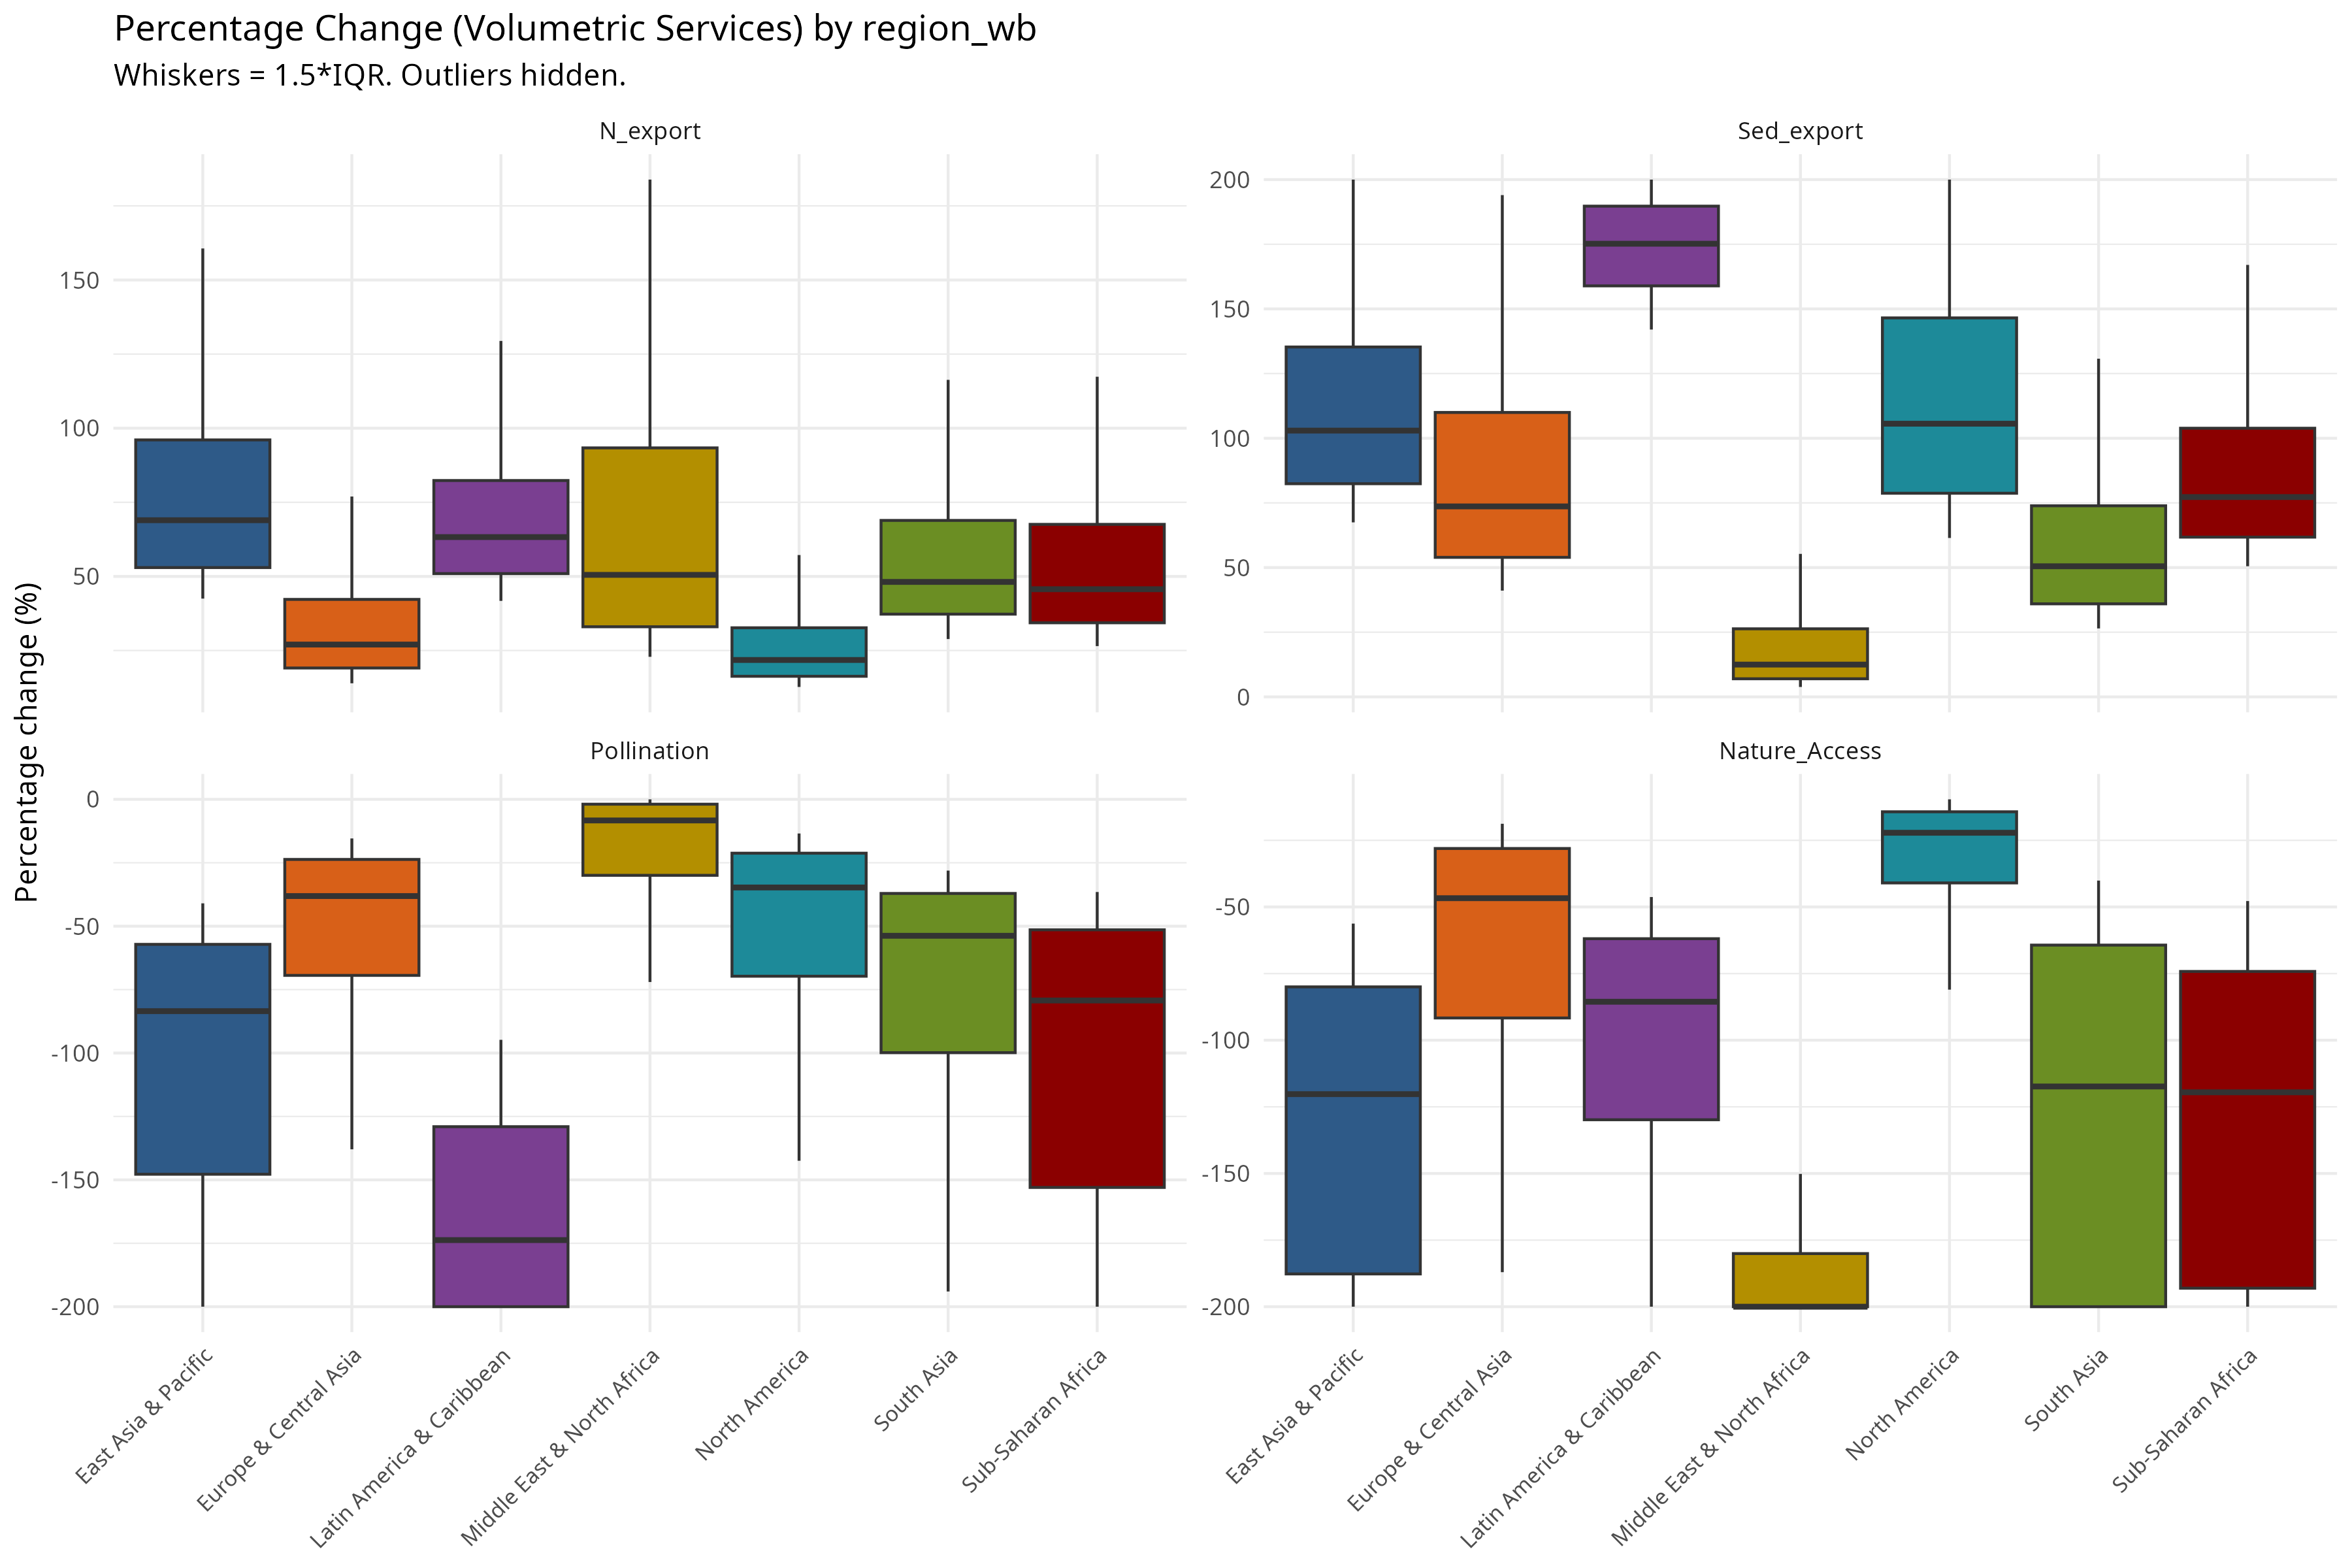
\includegraphics[keepaspectratio]{../outputs/plots/pct/region_wb/boxplots_region_wb_pct_volumetric.png}}

\pandocbounded{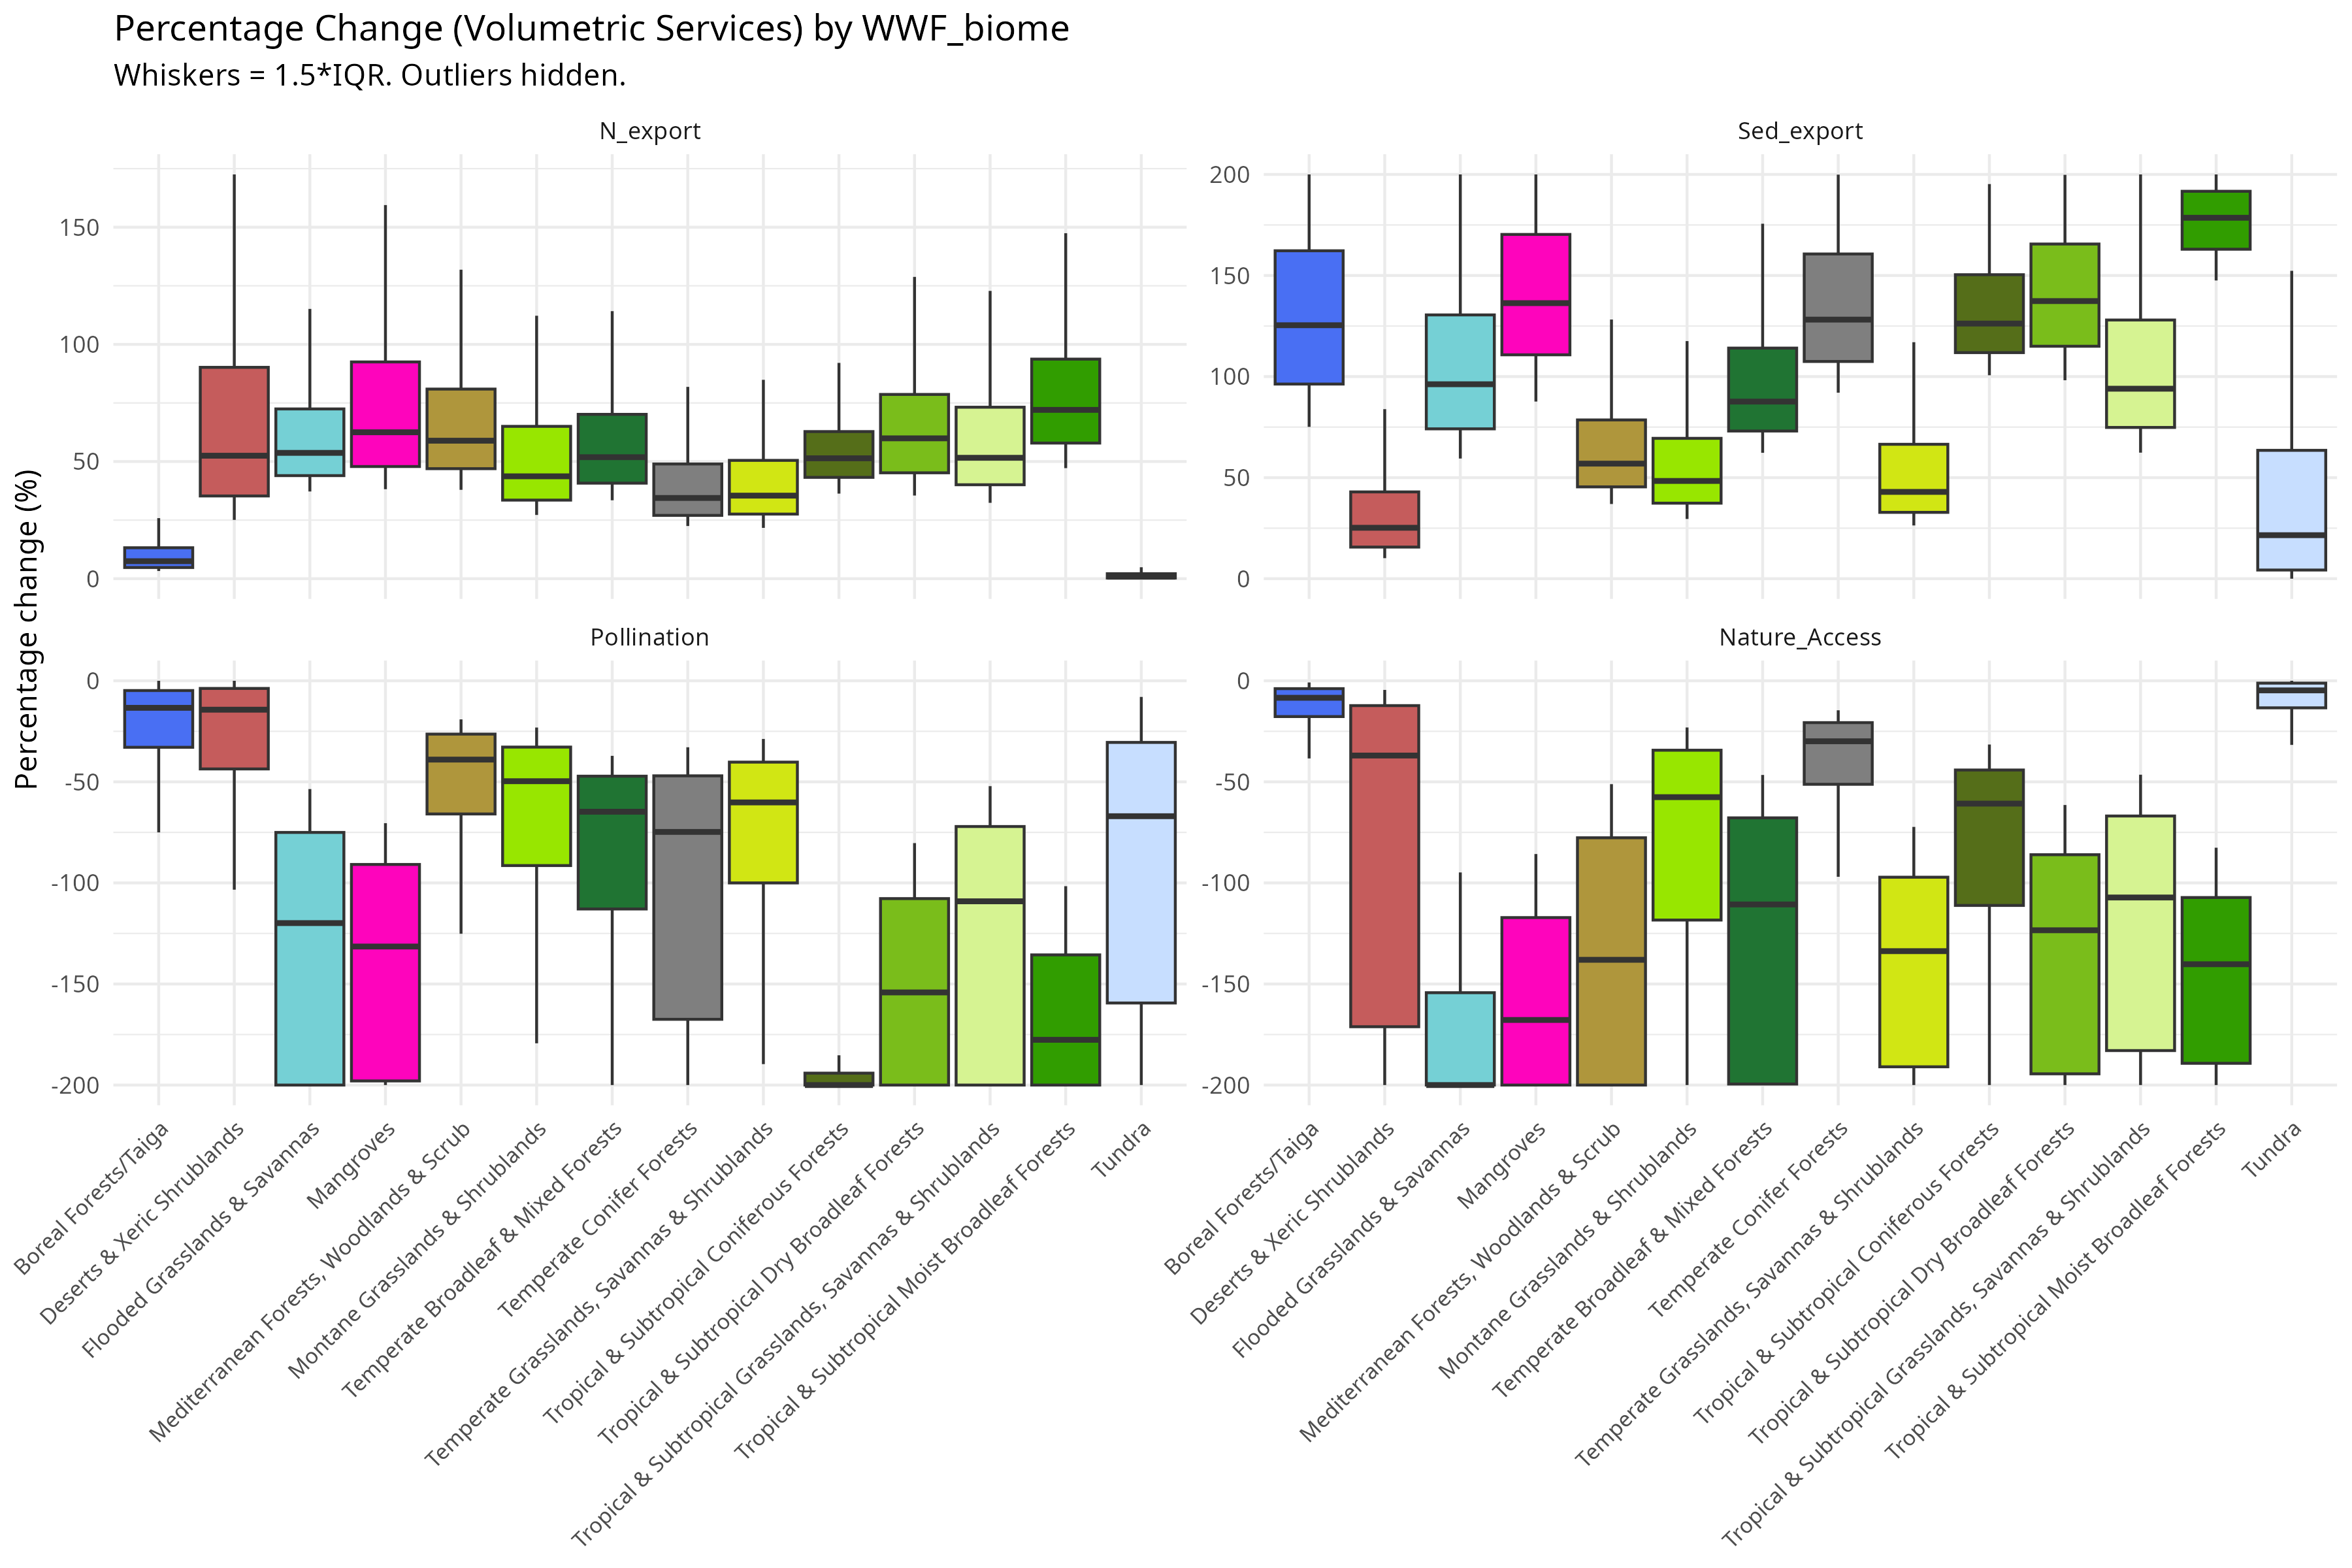
\includegraphics[keepaspectratio]{../outputs/plots/pct/wwf_biome/boxplots_wwf_biome_pct_volumetric.png}}

\pandocbounded{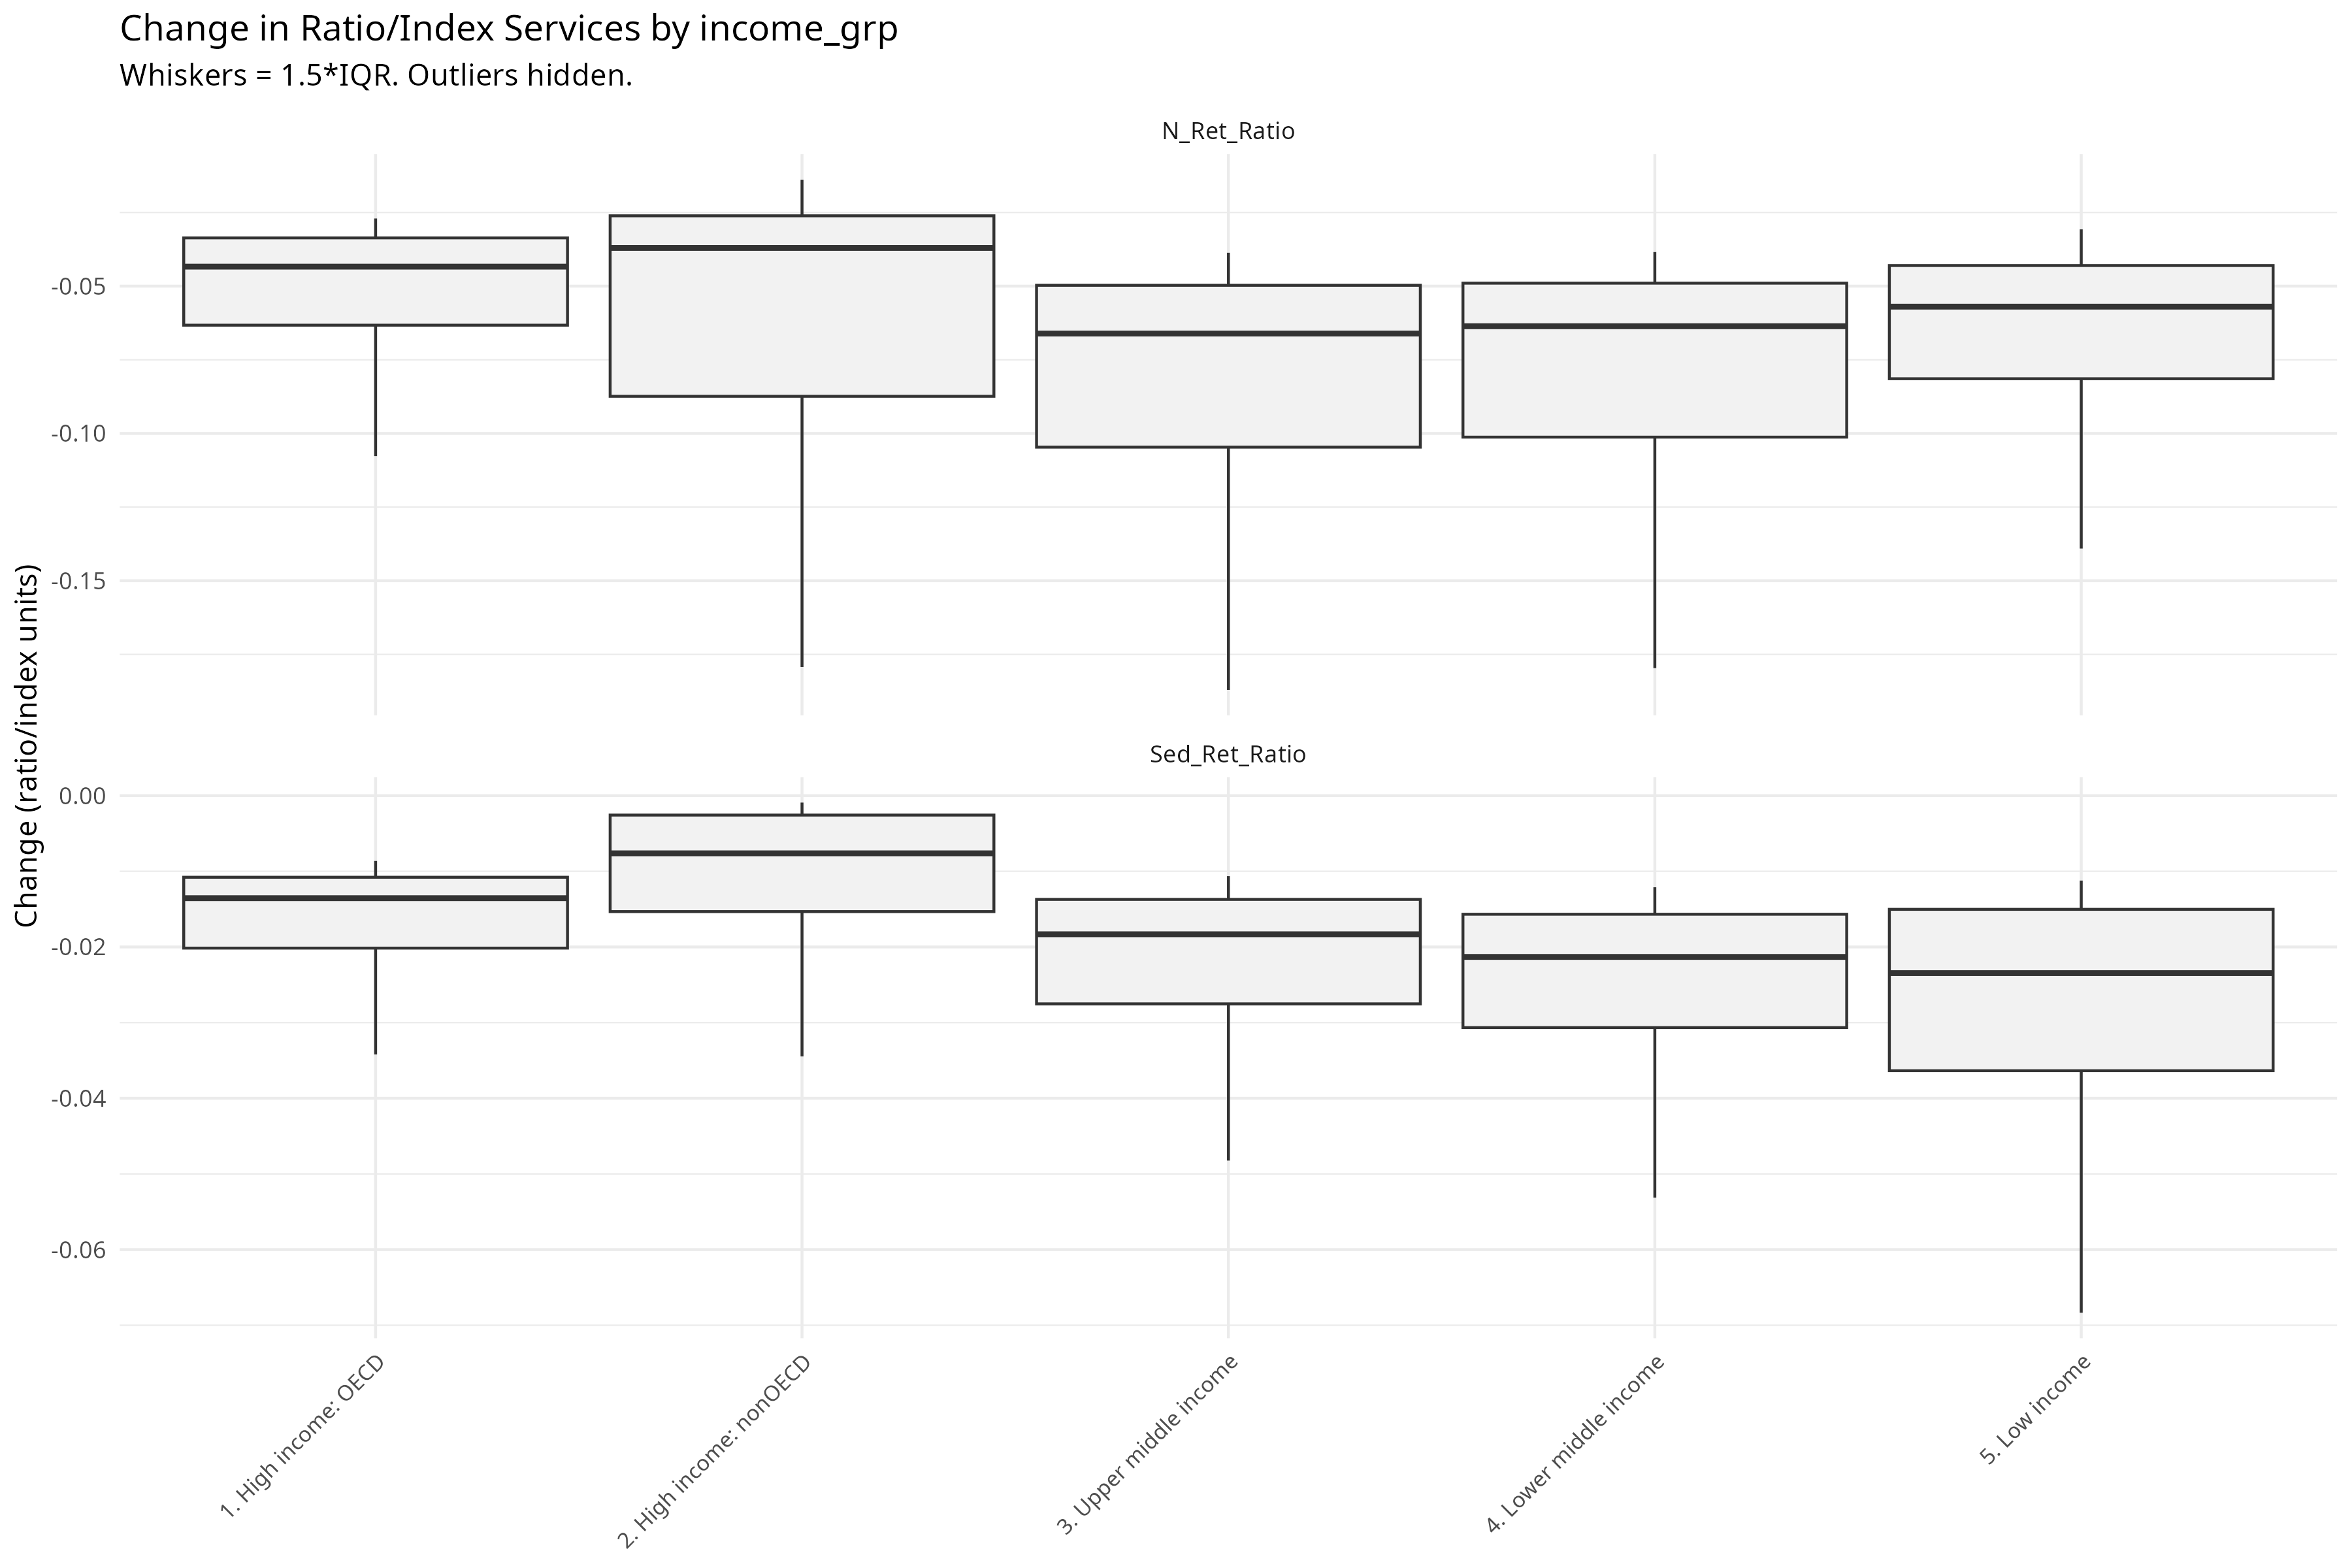
\includegraphics[keepaspectratio]{../outputs/plots/ratios/income_grp/boxplots_income_grp_ratios.png}}

\pandocbounded{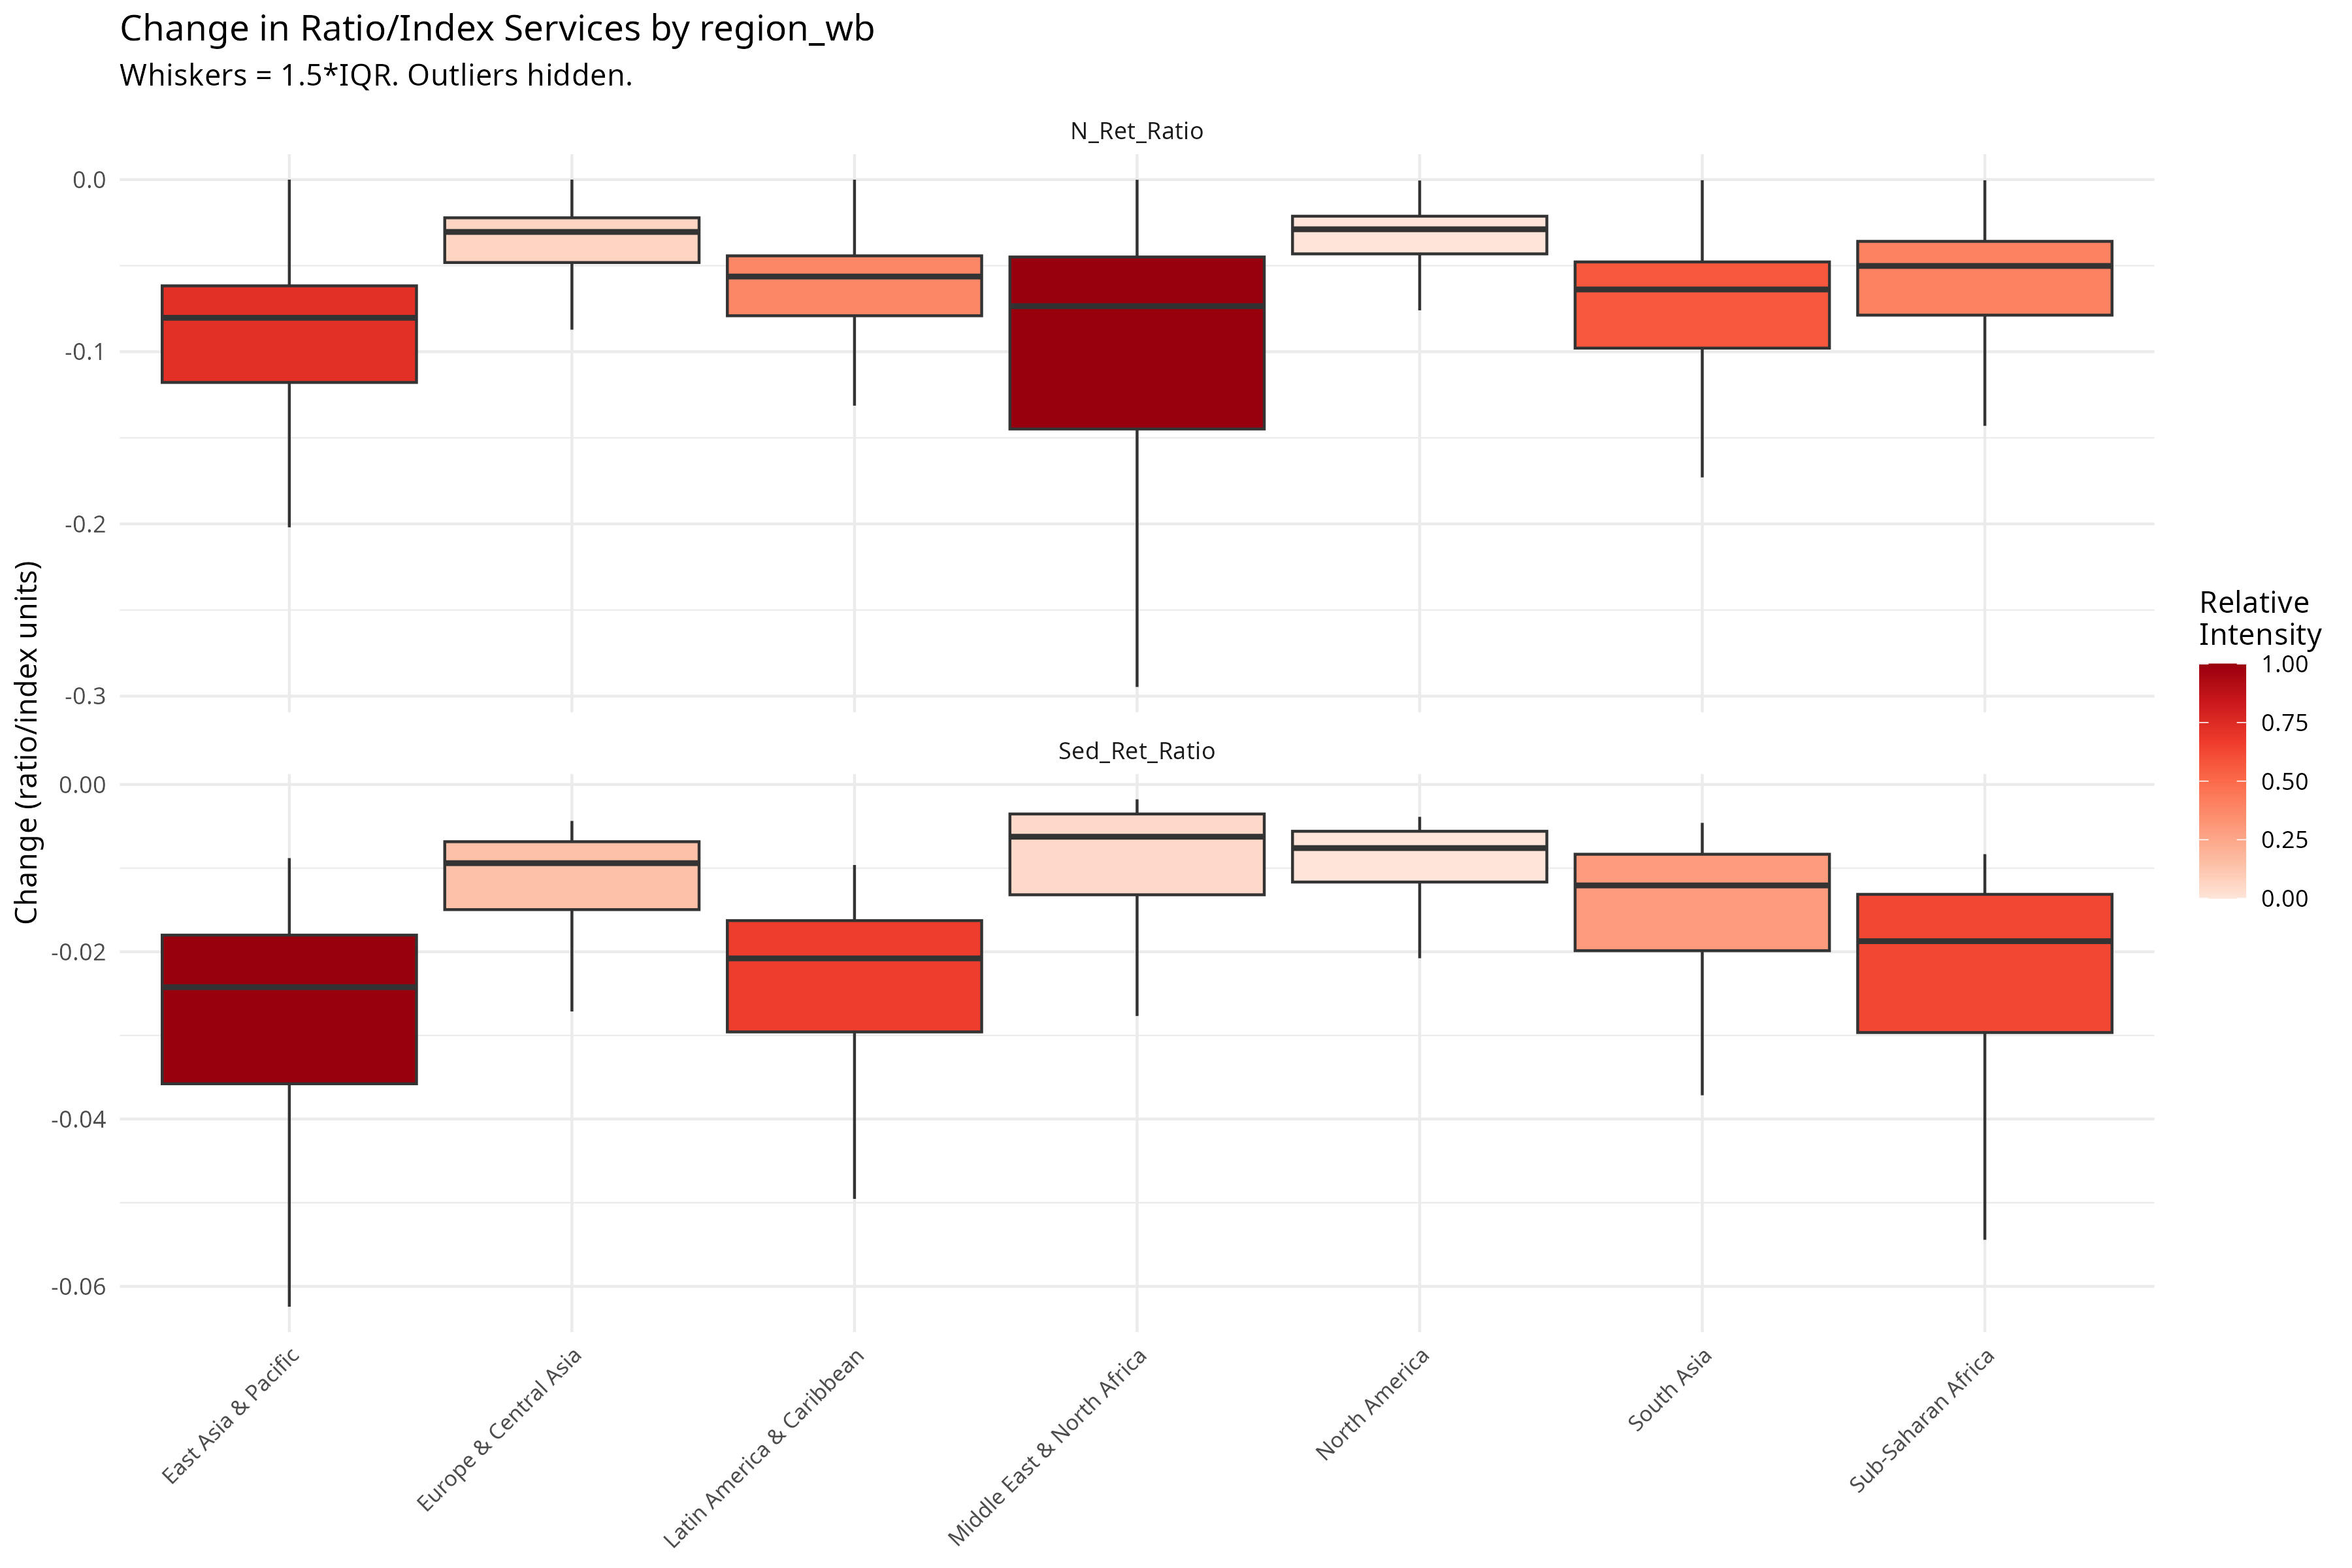
\includegraphics[keepaspectratio]{../outputs/plots/ratios/region_wb/boxplots_region_wb_ratios.png}}

\pandocbounded{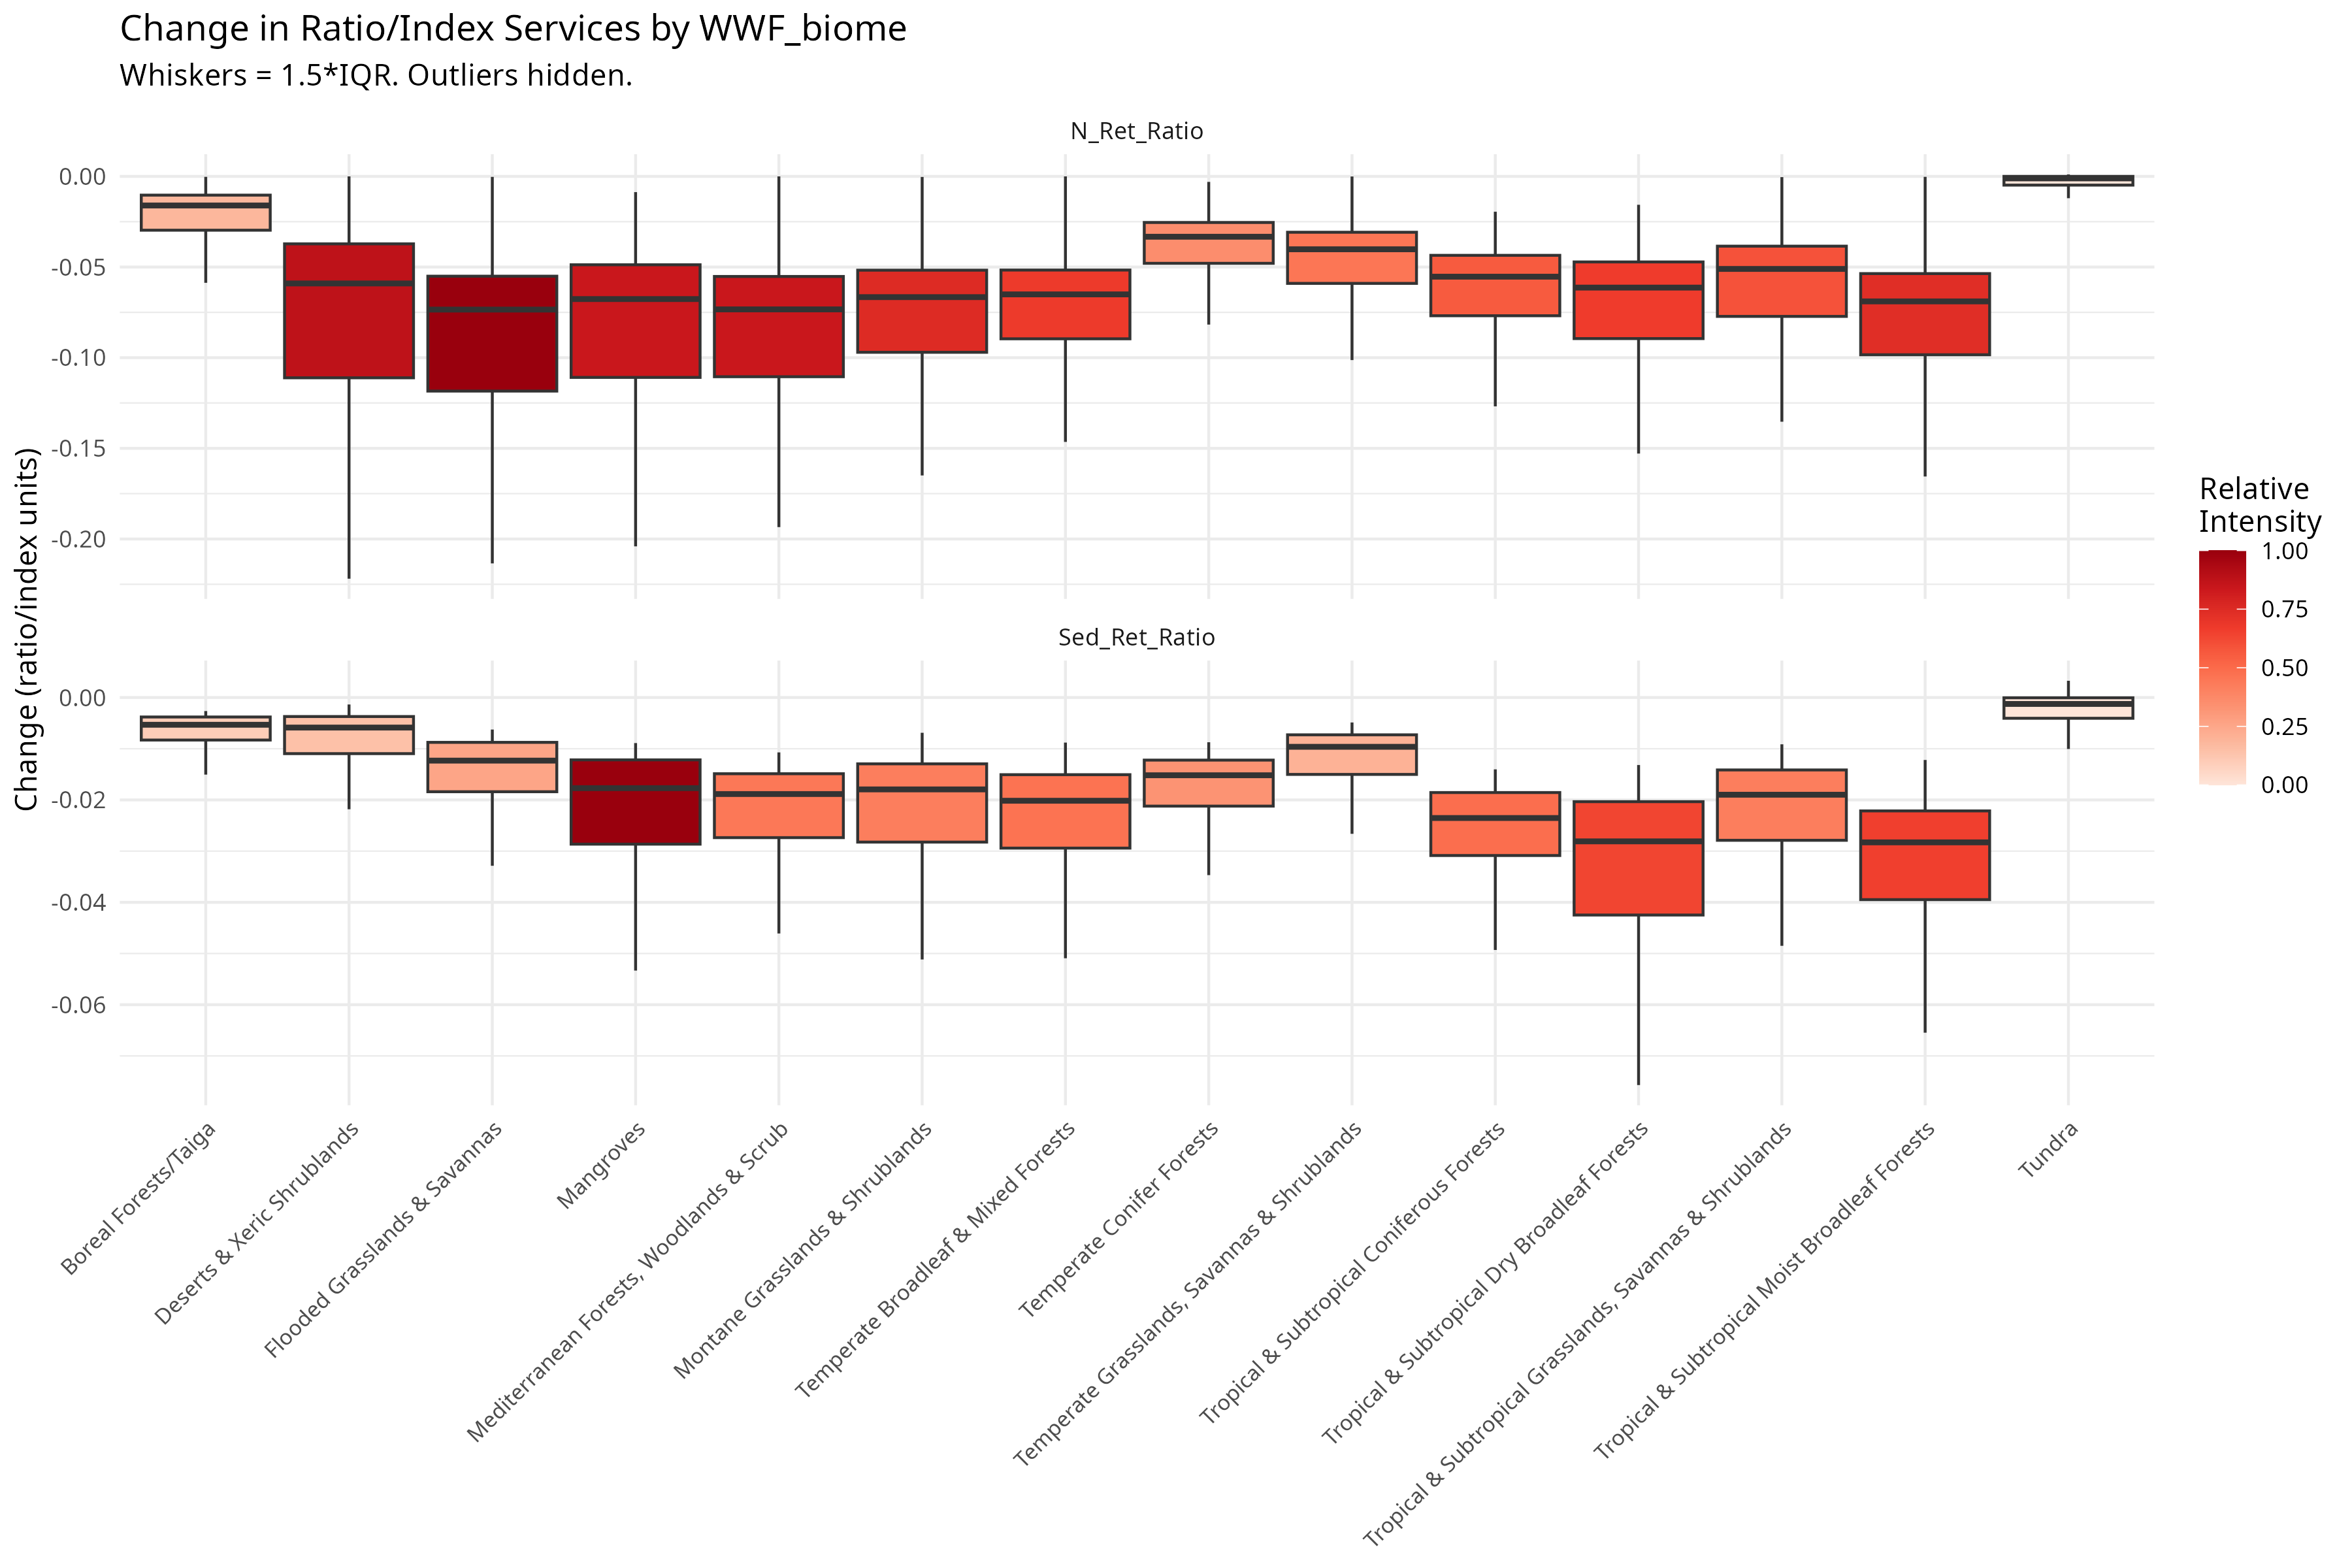
\includegraphics[keepaspectratio]{../outputs/plots/ratios/wwf_biome/boxplots_wwf_biome_ratios.png}}

\section{Attribution to Drivers of
Change}\label{attribution-to-drivers-of-change}

Here we integrate Land Cover change, specifically focusing on Land
Conversion (Loss of Natural Land). We define Conversion Hotspots as the
top 5\% of grid cells with the highest gross loss of natural land
(Loss\_2). We then calculate the overlap: What percentage of ES hotspots
are also Conversion Hotspots?

\begin{verbatim}


Table: LCC Attribution Gap (% Overlap) - pct_chg

|service          | n_es_hotspots| n_overlap| pct_overlap|driver      |metric  |
|:----------------|-------------:|---------:|-----------:|:-----------|:-------|
|Sed_Ret_Ratio    |         58025|     27072|        46.7|Forest_Loss |pct_chg |
|Nature_Access    |         75387|     32174|        42.7|Crop_Exp    |pct_chg |
|Sed_Ret_Ratio    |         58025|     24175|        41.7|Crop_Exp    |pct_chg |
|Sed_export       |         76309|     29779|        39.0|Forest_Loss |pct_chg |
|N_export         |         76309|     26713|        35.0|Forest_Loss |pct_chg |
|N_export         |         76309|     26071|        34.2|Crop_Exp    |pct_chg |
|Sed_export       |         76309|     22238|        29.1|Crop_Exp    |pct_chg |
|Nature_Access    |         75387|     20533|        27.2|Forest_Loss |pct_chg |
|Pollination      |         76309|     17739|        23.2|Forest_Loss |pct_chg |
|Pollination      |         76309|     16118|        21.1|Crop_Exp    |pct_chg |
|N_Ret_Ratio      |         57140|      8632|        15.1|Forest_Loss |pct_chg |
|N_Ret_Ratio      |         57140|      7128|        12.5|Crop_Exp    |pct_chg |
|C_Risk_Red_Ratio |          4242|       449|        10.6|Urban_Exp   |pct_chg |
|C_Risk           |          4243|       429|        10.1|Urban_Exp   |pct_chg |
|N_Ret_Ratio      |         57140|      3946|         6.9|Urban_Exp   |pct_chg |
|C_Risk           |          4243|       274|         6.5|Forest_Loss |pct_chg |
|Nature_Access    |         75387|      4475|         5.9|Urban_Exp   |pct_chg |
|C_Risk_Red_Ratio |          4242|       249|         5.9|Forest_Loss |pct_chg |
|C_Risk           |          4243|       174|         4.1|Crop_Exp    |pct_chg |
|C_Risk_Red_Ratio |          4242|       165|         3.9|Crop_Exp    |pct_chg |


Table: LCC Attribution Gap (% Overlap) - abs_chg

|service          | n_es_hotspots| n_overlap| pct_overlap|driver      |metric  |
|:----------------|-------------:|---------:|-----------:|:-----------|:-------|
|Sed_Ret_Ratio    |         58025|     27768|        47.9|Forest_Loss |abs_chg |
|Sed_Ret_Ratio    |         58025|     24548|        42.3|Crop_Exp    |abs_chg |
|N_export         |         76309|     21740|        28.5|Crop_Exp    |abs_chg |
|Sed_export       |         76309|     18344|        24.0|Forest_Loss |abs_chg |
|N_export         |         76309|     17754|        23.3|Forest_Loss |abs_chg |
|Sed_export       |         76309|     16000|        21.0|Crop_Exp    |abs_chg |
|Nature_Access    |         75387|     15608|        20.7|Crop_Exp    |abs_chg |
|N_Ret_Ratio      |         57140|      9893|        17.3|Forest_Loss |abs_chg |
|Nature_Access    |         75387|     12690|        16.8|Forest_Loss |abs_chg |
|Pollination      |         76309|     12324|        16.2|Crop_Exp    |abs_chg |
|Pollination      |         76309|     11917|        15.6|Forest_Loss |abs_chg |
|N_Ret_Ratio      |         57140|      7880|        13.8|Crop_Exp    |abs_chg |
|Nature_Access    |         75387|      7713|        10.2|Urban_Exp   |abs_chg |
|C_Risk_Red_Ratio |          4242|       426|        10.0|Urban_Exp   |abs_chg |
|C_Risk           |          4242|       421|         9.9|Urban_Exp   |abs_chg |
|N_Ret_Ratio      |         57140|      3881|         6.8|Urban_Exp   |abs_chg |
|C_Risk_Red_Ratio |          4242|       271|         6.4|Forest_Loss |abs_chg |
|C_Risk           |          4242|       270|         6.4|Forest_Loss |abs_chg |
|C_Risk           |          4242|       175|         4.1|Crop_Exp    |abs_chg |
|C_Risk_Red_Ratio |          4242|       170|         4.0|Crop_Exp    |abs_chg |
\end{verbatim}

\pandocbounded{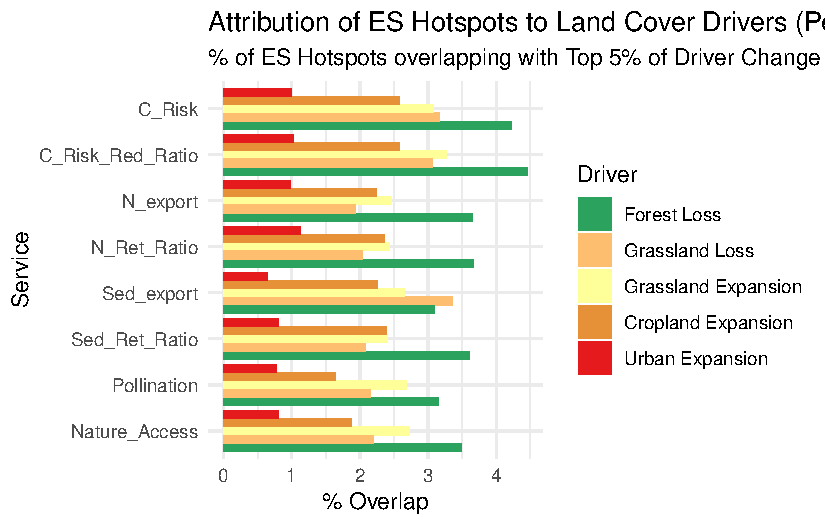
\includegraphics[keepaspectratio]{hotspot_extraction_files/figure-pdf/lc-hotspot-overlap-plot-1.pdf}}

\pandocbounded{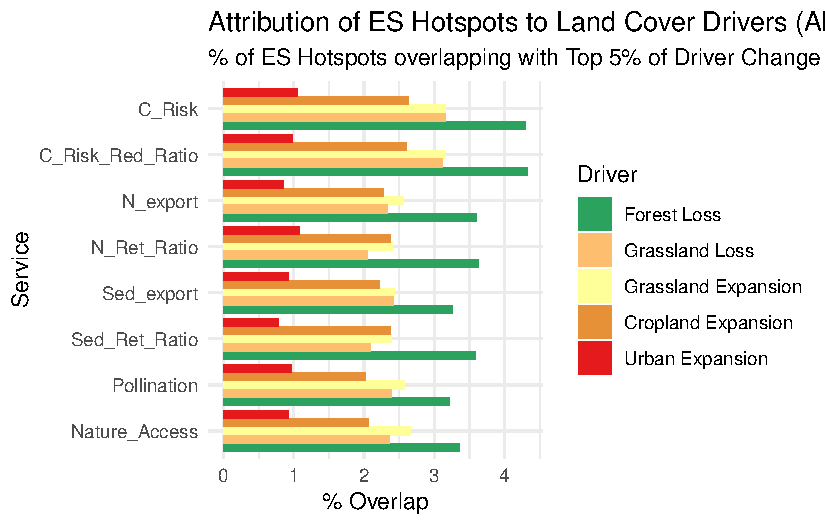
\includegraphics[keepaspectratio]{hotspot_extraction_files/figure-pdf/lc-hotspot-overlap-plot-2.pdf}}

\begin{verbatim}


Table: Correlation between ES Percentage Change and Net Natural Land Change

|service          | pearson_r| spearman_rho|       n|
|:----------------|---------:|------------:|-------:|
|Sed_Ret_Ratio    |     0.379|        0.724|  855968|
|Sed_export       |    -0.631|       -0.623| 1052572|
|N_export         |    -0.578|       -0.504| 1052572|
|Nature_Access    |     0.379|        0.425| 1043419|
|Pollination      |     0.275|        0.256| 1052572|
|N_Ret_Ratio      |     0.134|        0.217|  847609|
|C_Risk           |    -0.065|       -0.005|   59603|
|C_Risk_Red_Ratio |     0.051|        0.004|   59603|
\end{verbatim}

\pandocbounded{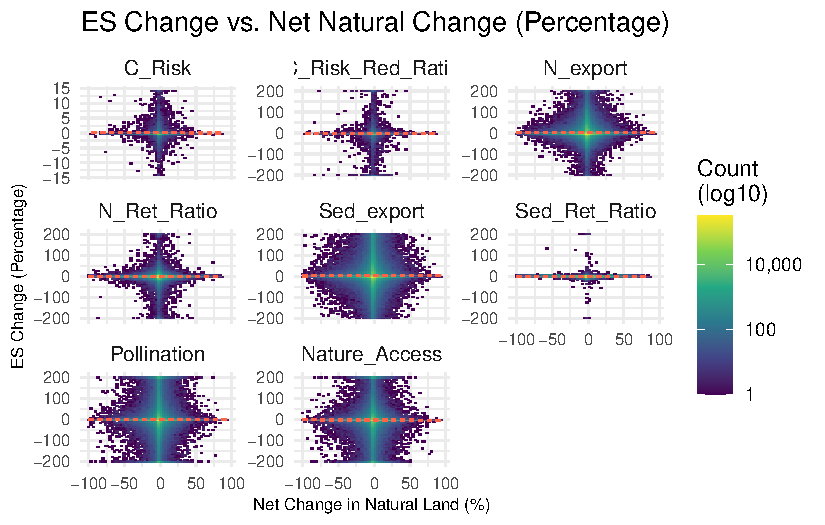
\includegraphics[keepaspectratio]{hotspot_extraction_files/figure-pdf/lc-es-correlation-1.pdf}}

\begin{verbatim}


Table: Correlation between ES Absolute Change and Net Natural Land Change

|service          | pearson_r| spearman_rho|       n|
|:----------------|---------:|------------:|-------:|
|Sed_Ret_Ratio    |     0.174|        0.726|  855968|
|Sed_export       |    -0.172|       -0.585| 1052572|
|N_export         |    -0.234|       -0.492| 1052572|
|Nature_Access    |     0.071|        0.418| 1043419|
|Pollination      |     0.019|        0.229| 1052572|
|N_Ret_Ratio      |     0.188|        0.219|  847609|
|C_Risk           |    -0.061|       -0.005|   59603|
|C_Risk_Red_Ratio |     0.065|        0.004|   59603|
\end{verbatim}

\pandocbounded{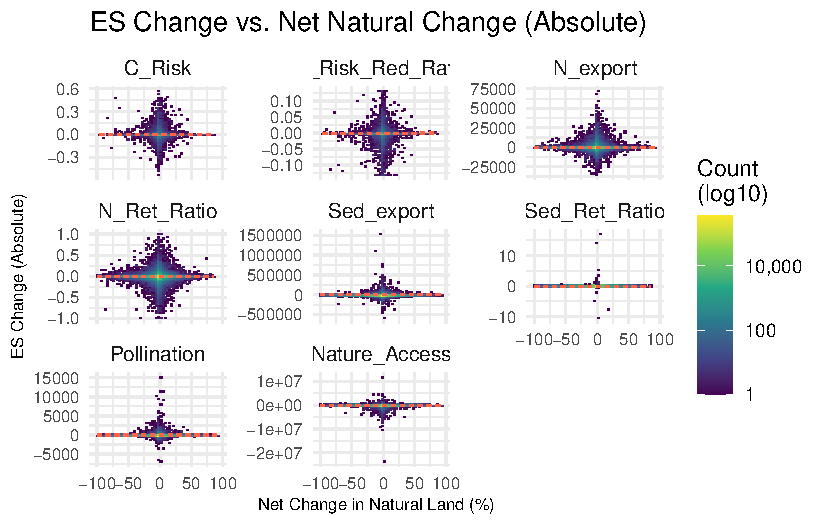
\includegraphics[keepaspectratio]{hotspot_extraction_files/figure-pdf/lc-es-correlation-2.pdf}}

\pandocbounded{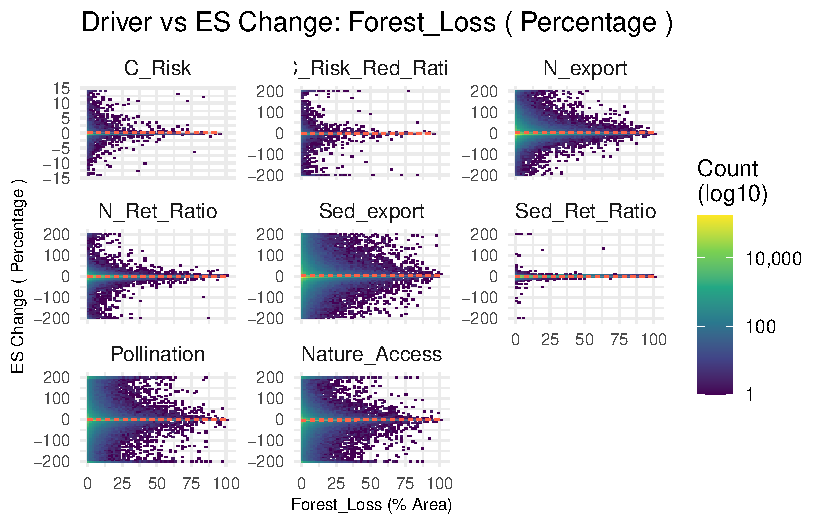
\includegraphics[keepaspectratio]{hotspot_extraction_files/figure-pdf/lc-es-scatterplots-1.pdf}}

\pandocbounded{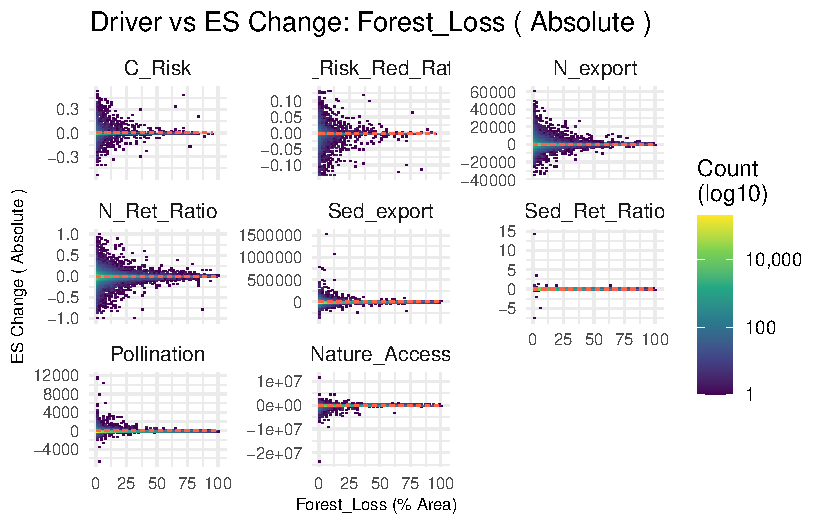
\includegraphics[keepaspectratio]{hotspot_extraction_files/figure-pdf/lc-es-scatterplots-2.pdf}}

\pandocbounded{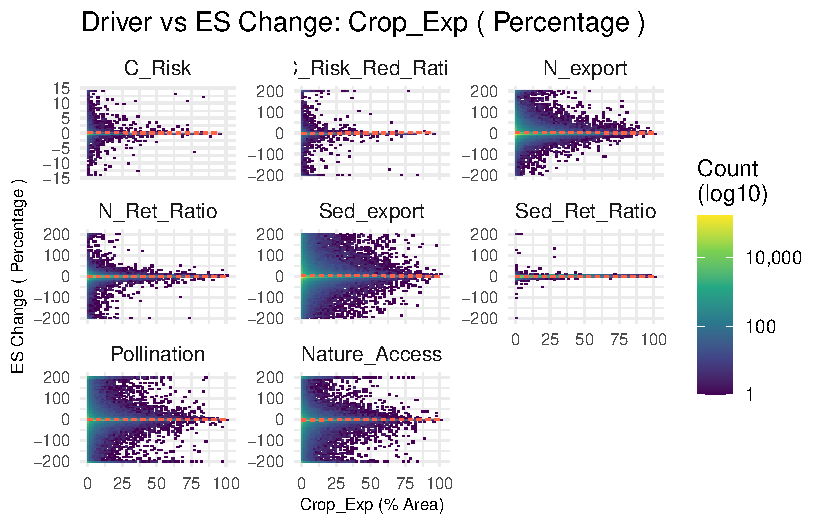
\includegraphics[keepaspectratio]{hotspot_extraction_files/figure-pdf/lc-es-scatterplots-3.pdf}}

\pandocbounded{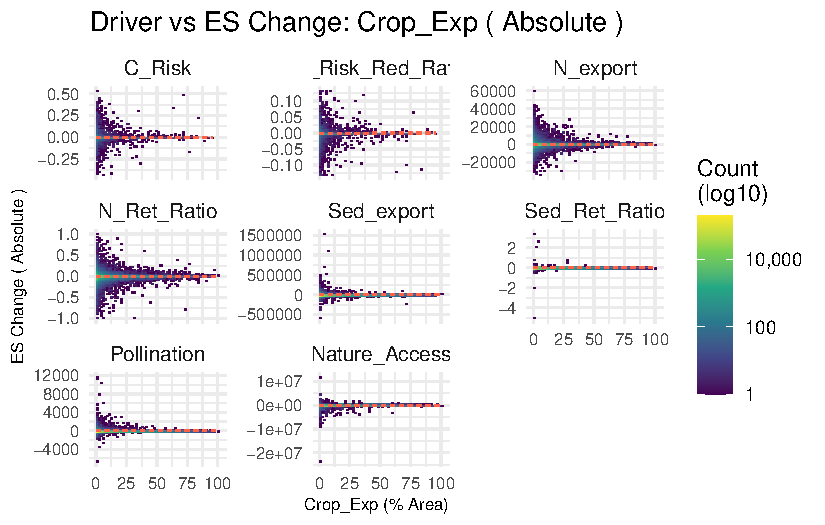
\includegraphics[keepaspectratio]{hotspot_extraction_files/figure-pdf/lc-es-scatterplots-4.pdf}}

\pandocbounded{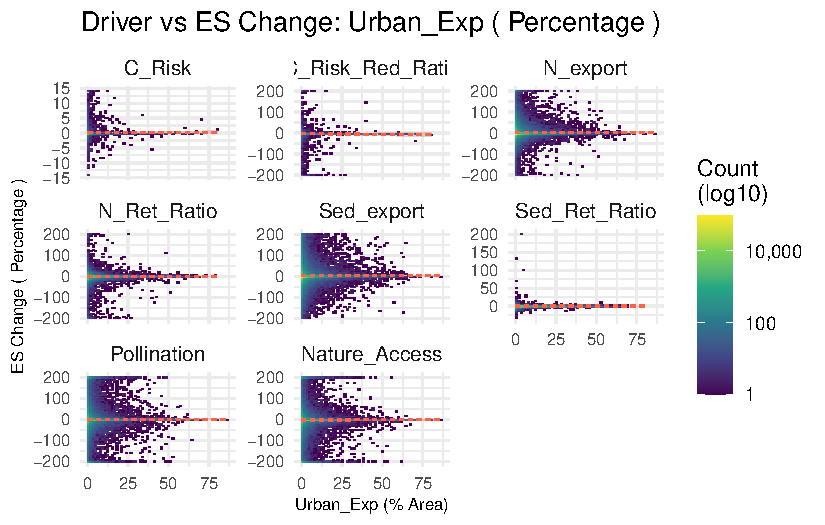
\includegraphics[keepaspectratio]{hotspot_extraction_files/figure-pdf/lc-es-scatterplots-5.pdf}}

\pandocbounded{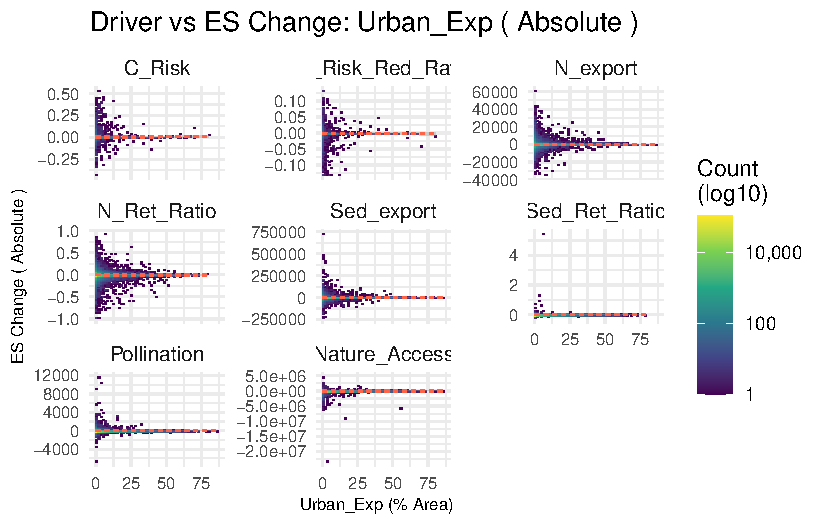
\includegraphics[keepaspectratio]{hotspot_extraction_files/figure-pdf/lc-es-scatterplots-6.pdf}}

\begin{verbatim}
Found socio vars: hdi_raster_predictions_2020_mean, rast_adm1_gini_disp_2020_mean, GHS_POP_E2020_GLOBE_sum, GlobPOP_Count_30arc_2020_sum, rast_gdpTot_1990_2020_30arcsec_2020_sum
\end{verbatim}

\begin{verbatim}


Table: Correlation: LC Drivers vs Socioeconomic Status

|Driver      |SocioVar                                | SpearmanRho|
|:-----------|:---------------------------------------|-----------:|
|Urban_Exp   |rast_gdpTot_1990_2020_30arcsec_2020_sum |       0.333|
|Urban_Exp   |GlobPOP_Count_30arc_2020_sum            |       0.320|
|Urban_Exp   |GHS_POP_E2020_GLOBE_sum                 |       0.309|
|Urban_Exp   |hdi_raster_predictions_2020_mean        |       0.149|
|Forest_Loss |hdi_raster_predictions_2020_mean        |       0.116|
|Forest_Loss |rast_adm1_gini_disp_2020_mean           |      -0.102|
|Urban_Exp   |rast_adm1_gini_disp_2020_mean           |      -0.062|
|Forest_Loss |rast_gdpTot_1990_2020_30arcsec_2020_sum |       0.047|
|Crop_Exp    |rast_adm1_gini_disp_2020_mean           |       0.036|
|Forest_Loss |GHS_POP_E2020_GLOBE_sum                 |       0.027|
|Crop_Exp    |rast_gdpTot_1990_2020_30arcsec_2020_sum |       0.020|
|Crop_Exp    |GHS_POP_E2020_GLOBE_sum                 |       0.016|
|Crop_Exp    |hdi_raster_predictions_2020_mean        |       0.004|
|Forest_Loss |GlobPOP_Count_30arc_2020_sum            |      -0.002|
|Crop_Exp    |GlobPOP_Count_30arc_2020_sum            |       0.000|
\end{verbatim}




\end{document}
